%%%  این قالب برر اساس قالب پایان‌نامۀ دانشگاه صنعتی امیرکبیر تهران و برای استفاده در دانشگاه صنعتی خواجه نصیرالدین طوسی توسعه داده شده است.
%%% https://github.com/MJAHMADEE/KNTUThesis

%%% مواردی که نسبت به قبل بروزرسانی شده است به شرح زیر می باشد
%%% 1- بولد شدن سر فصل ها
%%% 2- اضافه شدن قابلیت
%%%    \begin{subfigure}
%%% 3-   اصلاح ترتیب شماره گذاری مراجع به ترتیب اولویت ارجاع در متن 
%%% 4- مرتب شدن فایل‌ها (قرار گرفتن عکس ها و فونت ها در پوشه ای جداگانه)
%%% 5- اضافه شدن پکیج فرض
%%% 6- اضافه شدن فونت یاس برای فارسی شدن اعداد
%%% 7- اضافه شدن پکیج تنظیم سایز جدول


%%%  کلاس KNTUthesis، نسخه آبان 1397
%%%   دانشگاه صنعتی خواجه نصیرالدین طوسی                 http://www.KNTU.ac.ir
%%%
%%%

%-----------------------------------------------------------------------------------------------------
%        روش اجرا.: 2 بار F1 ، 2 بار  F11(به منظور تولید مراجع) ، دوبار Ctrl+Alt+I (به منظور تولید نمایه) و دو بار F1 -------> مشاهده Pdf
%%%%%%%%%%%%%%%%%%%%%%%%%%%%%%%%%%%%%%%%%%%%%%%%%%%%%%
%   TeXstudio as your IDE
%%  برای compile در TeXstudio تنها کافی است منوی Options->Configure TeXstudio را زده و در پنجره Configure TeXstudio در بخش Build گزینه Default Compiler را به XeLaTeX تغییر دهید. سند شما به راحتی compile خواهد شد.
%   F1 & F5 : Build & view
%   F6      : Compile
%   F7      : View
%   --------------
%%%%%%%%%%%%%%%%%%%%%%%%%%%%%%%%%%%%%%%%%%%%%%%%%%%%%%
%        اگر قصد نوشتن رساله دکتری را دارید، در خط زیر به جای msc،
%      کلمه phd را قرار دهید. کلیه تنظیمات لازم، به طور خودکار، اعمال می‌شود.
%%% !TEX TS-program = XeLaTeX
\documentclass[oneside,bsc,12pt]{KNTUthesis}
%       فایل commands.tex را حتماً به دقت مطالعه کنید؛ چون دستورات مربوط به فراخوانی بسته زی‌پرشین 
%       و دیگر بسته‌ها و ... در این فایل قرار دارد و بهتر است که با نحوه استفاده از آنها آشنا شوید. توجه شود برای نسخه نهایی پایان‌نامه حتماً hyperref را 
%        غیرفعال کنید.


% در این فایل، دستورها و تنظیمات مورد نیاز، آورده شده است.
%-------------------------------------------------------------------------------------------------------------------
\usepackage{listings}
% در ورژن جدید زی‌پرشین برای تایپ متن‌های ریاضی، این سه بسته، حتماً باید فراخوانی شود.
\usepackage{amsthm,amssymb,amsmath,amsfonts}
% بسته‌ای برای تنطیم حاشیه‌های بالا، پایین، چپ و راست صفحه
\usepackage[top=30mm, bottom=30mm, left=25mm, right=30mm]{geometry}
% بسته‌‌ای برای ظاهر شدن شکل‌ها و تصاویر متن
\usepackage{graphicx}
\usepackage{color}
%بسته‌ای برای تنظیم فاصله عمودی خط‌های متن
\usepackage{setspace}
\usepackage{titletoc}
\usepackage{tocloft}
\usepackage[utf8]{inputenc}
\usepackage{microtype}
\sloppy
\usepackage{tikz}
\usetikzlibrary{trees}
\usepackage{tcolorbox}
\usepackage{xcolor}
\usepackage{array}
\usepackage{caption}
\usepackage{float}
\usepackage[perpage]{footmisc} % Reset footnote counter on each page
%با فعال کردن بسته زیر فوت‌نوت‌ها در هر صفحه ریست می‌شوند. حالت پیش‌فرض آن ریست شدن در هر فصل می‌باشد.
%\usepackage[perpage]{footmisc}
\usepackage{enumitem}
\usepackage{multirow,adjustbox}
%\usepackage{titlesec}
% بسته‌ و دستوراتی برای ایجاد لینک‌های رنگی با امکان جهش
\usepackage[pagebackref=false,colorlinks,linkcolor=blue,citecolor=red]{hyperref}
\usepackage[nameinlink]{cleveref}%capitalize,,noabbrev
 \AtBeginDocument{%
    \crefname{equation}{برابری}{equations}%
    \crefname{chapter}{فصل}{chapters}%
    \crefname{section}{بخش}{sections}%
    \crefname{appendix}{پیوست}{appendices}%
    \crefname{enumi}{مورد}{items}%
    \crefname{footnote}{زیرنویس}{footnotes}%
    \crefname{figure}{شکل}{figures}%
    \crefname{table}{جدول}{tables}%
    \crefname{theorem}{قضیه}{theorems}%
    \crefname{lemma}{لم}{lemmas}%
    \crefname{corollary}{نتیجه}{corollaries}%
    \crefname{proposition}{گزاره}{propositions}%
    \crefname{definition}{تعریف}{definitions}%
    \crefname{result}{نتیجه}{results}%
    \crefname{example}{مثال}{examples}%
    \crefname{remark}{نکته}{remarks}%
    \crefname{note}{یادداشت}{notes}%
    \crefname{asum}{فرض}{Assumption}
    % دستوری برای تغییر نام کلمه «کتاب‌نامه» به «منابع و مراجع«
    \renewcommand{\bibname}{منابع و مراجع}
    
    \renewcommand{\labelitemi}{$\bullet$}
    % دستوری برای تعیین علامت سطح دوم itemize
    \renewcommand{\labelitemii}{$\circ$}
    % دستوری برای تعیین علامت سطح سوم itemize
    \renewcommand{\labelitemiii}{$-$}
    % برای سطح چهارم
    \renewcommand{\labelitemiv}{$*$}
    % دستوری برای تغییر نام کلمه «اثبات» به «برهان»
    \renewcommand\proofname{\textbf{برهان}}
    \renewcommand{\listfigurename}{فهرست اشکال}
    \renewcommand{\listtablename}{فهرست جداول}
}

\usepackage{subcaption}
% چنانچه قصد پرینت گرفتن نوشته خود را دارید، خط بالا را غیرفعال و  از دستور زیر استفاده کنید چون در صورت استفاده از دستور زیر‌‌، 
% لینک‌ها به رنگ سیاه ظاهر خواهند شد که برای پرینت گرفتن، مناسب‌تر است
%\usepackage[pagebackref=false]{hyperref}
% بسته‌ لازم برای تنظیم سربرگ‌ها
\usepackage{fancyhdr}
% بسته‌ای برای ظاهر شدن «مراجع»  در فهرست مطالب
\usepackage[nottoc]{tocbibind}
% دستورات مربوط به ایجاد نمایه
\usepackage{makeidx,multicol}
\setlength{\columnsep}{1.5cm}

%%%%%%%%%%%%%%%%%%%%%%%%%%
\usepackage{verbatim}
\makeindex
\usepackage{sectsty}
% فراخوانی بسته زی‌پرشین و تعریف قلم فارسی و انگلیسی
\usepackage{xepersian}%[extrafootnotefeatures]
\SepMark{-}
%حتماً از تک لایو 2014 استفاده کنید.
\settextfont[Scale=1.2,Path=Fonts/,BoldFont=B Nazanin Bold.ttf]{B Nazanin.ttf}
\setlatintextfont[Path=Fonts/,BoldFont=timesbd]{times}

%%%%%%%%%%%%%%%%%%%%%%%%%%
% چنانچه می‌خواهید اعداد در فرمول‌ها، انگلیسی باشد، خط زیر را غیرفعال کنید.
%
\setdigitfont[Scale=1.1,Path=Fonts/,BoldFont=Yas Bd.ttf]{Yas.ttf}%%Yas
%%%%%%%%%%%%%%%%%%%%%%%%%%
% تعریف قلم‌های فارسی اضافی برای استفاده در بعضی از قسمت‌های متن
\defpersianfont\nastaliq[Scale=2,Path=Fonts/]{IranNastaliq.ttf}
\defpersianfont\chapternumber[Scale=3,Path=Fonts/,BoldFont=B Nazanin Bold.ttf]{B Nazanin.ttf}
%\chapterfont{\centering}%
%%%%%%%%%%%%%%%%%%%%%%%%%%





% Headings for every page of ToC, LoF and Lot
\setlength{\cftbeforetoctitleskip}{-1.2em}
\setlength{\cftbeforelottitleskip}{-1.2em}
\setlength{\cftbeforeloftitleskip}{-1.2em}
\setlength{\cftaftertoctitleskip}{-1em}
\setlength{\cftafterlottitleskip}{-1em}
\setlength{\cftafterloftitleskip}{-1em}
%%\makeatletter
%%%%\renewcommand{\l@chapter}{\@dottedtocline{1}{1em\bfseries}{1em}}
%%%%\renewcommand{\l@section}{\@dottedtocline{2}{2em}{2em}}
%%%%\renewcommand{\l@subsection}{\@dottedtocline{3}{3em}{3em}}
%%%%\renewcommand{\l@subsubsection}{\@dottedtocline{4}{4em}{4em}}
%%%%\makeatother


\newcommand\tocheading{\par عنوان\hfill صفحه \par}
\newcommand\lofheading{\hspace*{.5cm}\figurename\hfill صفحه \par}
\newcommand\lotheading{\hspace*{.5cm}\tablename\hfill صفحه \par}

\renewcommand{\cftchapleader}{\cftdotfill{\cftdotsep}}
\renewcommand{\cfttoctitlefont}{\hspace*{\fill}\LARGE\bfseries}%\Large
\renewcommand{\cftaftertoctitle}{\hspace*{\fill}}
\renewcommand{\cftlottitlefont}{\hspace*{\fill}\LARGE\bfseries}%\Large
\renewcommand{\cftafterlottitle}{\hspace*{\fill}}
\renewcommand{\cftloftitlefont}{\hspace*{\fill}\LARGE\bfseries}
\renewcommand{\cftafterloftitle}{\hspace*{\fill}}

%%%%%%%%%%%%%%%%%%%%%%%%%%
% تعریف و نحوه ظاهر شدن عنوان قضیه‌ها، تعریف‌ها، مثال‌ها و ...
%برای شماره گذاری سه تایی قضیه ها
\theoremstyle{definition}
\newtheorem{definition}{تعریف}[section]
\newtheorem{remark}[definition]{نکته}
\newtheorem{note}[definition]{یادداشت}
\newtheorem{example}[definition]{نمونه}
\newtheorem{question}[definition]{سوال}
\newtheorem{remember}[definition]{یاداوری}
\theoremstyle{theorem}
\newtheorem{theorem}[definition]{قضیه}
\newtheorem{lemma}[definition]{لم}
\newtheorem{proposition}[definition]{گزاره}
\newtheorem{corollary}[definition]{نتیجه}
\newtheorem{asum}[definition]{فرض}
%%%%%%%%%%%%%%%%%%%%%%%%
%%%%%%%%%%%%%%%%%%%
%%% برای شماره گذاری چهارتایی قضیه ها و ...
%%\newtheorem{definition1}[subsubsection]{تعریف}
%%\newtheorem{theorem1}[subsubsection]{قضیه}
%%\newtheorem{lemma1}[subsubsection]{لم}
%%\newtheorem{proposition1}[subsubsection]{گزاره}
%%\newtheorem{corollary1}[subsubsection]{نتیجه}
%%\newtheorem{remark1}[subsubsection]{نکته}
%%\newtheorem{example1}[subsubsection]{مثال}
%%\newtheorem{question1}[subsubsection]{سوال}

%%%%%%%%%%%%%%%%%%%%%%%%%%%%

% دستورهایی برای سفارشی کردن صفحات اول فصل‌ها
\makeatletter
\newcommand\mycustomraggedright{%
 \if@RTL\raggedleft%
 \else\raggedright%
 \fi}
\def\@makechapterhead#1{%
\thispagestyle{style1}
\vspace*{20\p@}%
{\parindent \z@ \mycustomraggedright
\ifnum \c@secnumdepth >\m@ne
\if@mainmatter

\bfseries{\Huge \@chapapp}\small\space {\chapternumber\thechapter}
\par\nobreak
\vskip 0\p@
\fi
\fi
\interlinepenalty\@M 
\Huge \bfseries #1\par\nobreak
\vskip 120\p@

}

%\thispagestyle{empty}
\newpage}
\bidi@patchcmd{\@makechapterhead}{\thechapter}{\tartibi{chapter}}{}{}
\bidi@patchcmd{\chaptermark}{\thechapter}{\tartibi{chapter}}{}{}
\makeatother

\pagestyle{fancy}
\renewcommand{\chaptermark}[1]{\markboth{\chaptername~\tartibi{chapter}: #1}{}}

\fancypagestyle{style1}{
\fancyhf{} 
\fancyfoot[c]{\thepage}
\fancyhead[R]{\leftmark}%
\renewcommand{\headrulewidth}{1.2pt}
}


\fancypagestyle{style2}{
\fancyhf{}
\fancyhead[R]{چکیده}
\fancyfoot[C]{\thepage{}}
\renewcommand{\headrulewidth}{1.2pt}
}

\fancypagestyle{style3}{%
  \fancyhf{}%
  \fancyhead[R]{فهرست نمادها}
  \fancyfoot[C]{\thepage}%
  \renewcommand{\headrulewidth}{1.2pt}%
}

\fancypagestyle{style4}{%
  \fancyhf{}%
  \fancyhead[R]{فهرست جداول}
  \fancyfoot[C]{\thepage}%
  \renewcommand{\headrulewidth}{1.2pt}%
}

\fancypagestyle{style5}{%
  \fancyhf{}%
  \fancyhead[R]{فهرست اشکال}
  \fancyfoot[C]{\thepage}%
  \renewcommand{\headrulewidth}{1.2pt}%
}

\fancypagestyle{style6}{%
  \fancyhf{}%
  \fancyhead[R]{فهرست مطالب}
  \fancyfoot[C]{\thepage}%
  \renewcommand{\headrulewidth}{1.2pt}%
}

\fancypagestyle{style7}{%
  \fancyhf{}%
  \fancyhead[R]{نمایه}
  \fancyfoot[C]{\thepage}%
  \renewcommand{\headrulewidth}{1.2pt}%
}

\fancypagestyle{style8}{%
  \fancyhf{}%
  \fancyhead[R]{منابع و مراجع}
  \fancyfoot[C]{\thepage}%
  \renewcommand{\headrulewidth}{1.2pt}%
}
\fancypagestyle{style9}{%
  \fancyhf{}%
  \fancyhead[R]{واژه‌نامه‌ی فارسی به انگلیسی}
  \fancyfoot[C]{\thepage}%
  \renewcommand{\headrulewidth}{1.2pt}%
}
%


%دستور حذف نام لیست تصاویر و لیست جداول از فهرست مطالب
\newcommand*{\BeginNoToc}{%
  \addtocontents{toc}{%
    \edef\protect\SavedTocDepth{\protect\the\protect\value{tocdepth}}%
  }%
  \addtocontents{toc}{%
    \protect\setcounter{tocdepth}{-10}%
  }%
}
\newcommand*{\EndNoToc}{%
  \addtocontents{toc}{%
    \protect\setcounter{tocdepth}{\protect\SavedTocDepth}%
  }%
}
\newcounter{savepage}

%\renewcommand\cftsecleader{\cftdotfill{\cftdotsep}}
%%%%%%%%%%%%%%%%%%%%%%%%%%%%%

\newtcolorbox[auto counter,number within=section,
number freestyle={(\noexpand\arabic{\tcbcounter}-\thesection)},
]{phbox}[2][]{%
	colback=yellow!15!white,colframe=blue!75!black,fonttitle=\bfseries,
	title=تمرین~\thetcbcounter: #2,#1}

\newtcolorbox[auto counter,number within=section,
number freestyle={(\noexpand\arabic{\tcbcounter}-\thesection)},
]{phboxr}[2][]{%
	colback=yellow!15!white,colframe=red!75!black,fonttitle=\bfseries,
	title=توجه}

\newtcolorbox[auto counter,number within=section,
number freestyle={(\noexpand\arabic{\tcbcounter}-\thesection)},
]{phboxb}[2][]{%
	colback=yellow!15!white,colframe=blue!75!black,fonttitle=\bfseries,
	title=نکته}

\newtcolorbox[auto counter,number within=section,
number freestyle={(\noexpand\arabic{\tcbcounter}-\thesection)},
]{phboxb1}[2][]{%
	colback=white!15!white,colframe=black!75!black,fonttitle=\bfseries,
	title=انگیزه}


\newtcolorbox[auto counter,number within=section,
number freestyle={(\noexpand\arabic{\tcbcounter}-\thesection)},
]{phboxg}[2][]{%
	colback=yellow!15!white,colframe=green!75!black,fonttitle=\bfseries,
	title=جمع‌بندی}

\newtcolorbox[auto counter,number within=section,
number freestyle={(\noexpand\arabic{\tcbcounter}-\thesection)},
]{phboxgg}[2][]{%
	colback=yellow!15!white,colframe=green!75!black,fonttitle=\bfseries,
	title=جمع‌بندی روش‌های پیشنهادی اول و دوم}

\newtcolorbox[auto counter,number within=section,
number freestyle={(\noexpand\arabic{\tcbcounter}-\thesection)},
]{phboxp}[2][]{%
	colback=yellow!15!white,colframe=purple!75!black,fonttitle=\bfseries,
	title=هدف}

\newtcolorbox[auto counter,number within=section,
number freestyle={(\noexpand\arabic{\tcbcounter}-\thesection)},
]{phboxbr}[2][]{%
	colback=yellow!10!white,colframe=brown!95!black,fonttitle=\bfseries,
	title=محتوای کارگاه آموزشی لتک}

%%%%%%%%%%%%%%%%%%%%%%%%%%%%

\renewcommand{\lstlistingname}{Code}

\definecolor{codegreen}{rgb}{0,0.6,0}
\definecolor{codegray}{rgb}{0.5,0.5,0.5}
\definecolor{codepurple}{rgb}{0.58,0,0.82}
\definecolor{backcolour}{rgb}{0.95,0.95,0.92}

\lstdefinestyle{mystyle}{
	backgroundcolor=\color{backcolour},   
	commentstyle=\color{codegreen},
	keywordstyle=\color{magenta},
	numberstyle=\tiny\color{codegray},
	stringstyle=\color{codepurple},
	basicstyle=\ttfamily\footnotesize,
	breakatwhitespace=false,         
	breaklines=true,                 
	captionpos=b,                    
	keepspaces=true,                 
	numbers=left,                    
	numbersep=5pt,                  
	showspaces=false,                
	showstringspaces=false,
	showtabs=false,                  
	tabsize=2
}

\lstset{style=mystyle}

\begin{document}
\baselineskip=.75cm
\linespread{1.75}
%% -!TEX root = KNTUthesis.tex
% در این فایل، عنوان پایان‌نامه، مشخصات خود، متن تقدیمی‌، ستایش، سپاس‌گزاری و چکیده پایان‌نامه را به فارسی، وارد کنید.
% توجه داشته باشید که جدول حاوی مشخصات پروژه/پایان‌نامه/رساله و همچنین، مشخصات داخل آن، به طور خودکار، درج می‌شود.
%%%%%%%%%%%%%%%%%%%%%%%%%%%%%%%%%%%%
% دانشکده، آموزشکده و یا پژوهشکده  خود را وارد کنید
\faculty{دانشکده مهندسی برق}
% گرایش و گروه آموزشی خود را وارد کنید
\department{}
% عنوان پایان‌نامه را وارد کنید


\fatitle{پردازش تصاویر 
\lr{CT‌ Scan}
مغز به منظور قطعه‌بندی خونریزی داخلی مغز با استفاده از شبکه‌های عصبی عمیق
\\[.75 cm]
 پایان‌نامه کارشناسی}
% نام استاد(ان) راهنما را وارد کنید
\firstsupervisor{دکتر امیرحسین نیکوفرد}
%\secondsupervisor{استاد راهنمای دوم}
% نام استاد(دان) مشاور را وارد کنید. چنانچه استاد مشاور ندارید، دستور پایین را غیرفعال کنید.
%\firstadvisor{نام کامل استاد مشاور}
%\secondadvisor{استاد مشاور دوم}
% نام نویسنده را وارد کنید
\name{سید محمد }
% نام خانوادگی نویسنده را وارد کنید
\surname{حسینی}
%%%%%%%%%%%%%%%%%%%%%%%%%%%%%%%%%%
\thesisdate{شهریور 1403}

% چکیده پایان‌نامه را وارد کنید
\fa-abstract{
تشخیص سریع و دقیق خونریزی‌های درون‌جمجمه‌ای با استفاده از تصاویر سی‌تی‌اسکن، همواره به‌عنوان یکی از مهم‌ترین چالش‌های پزشکی در زمینه درمان افراد دارای انواع آسیب‌های مغزی، سکته‌های مغزی و خونریزی‌های درون‌جمجمه‌ای، مطرح شده است. اهمیت این موضوع زمانی آشکار می‌شود که حتی تأخیر چنددقیقه‌ای در تشخیص می‌تواند منجر به پیامدهای جبران‌ناپذیری برای بیماران شود.
باتوجه‌به پیچیدگی و حساسیت بالای تشخیص چنین آسیب‌هایی، این فرایند معمولاً نیازمند تخصص و تجربه‌ی بالای پزشکان و پرتوشناسان است. اما باتوجه‌به محدودیت منابع انسانی و احتمال خطاهای انسانی، نیاز به توسعه سامانه‌های خودکار تشخیص مبتنی بر یادگیری عمیق بیش‌ازپیش احساس می‌شود.
در این زمینه چالش اصلی برای پزشکان خصوصاً در بخش فوریت‌های پزشکی، تشخیص دقیق و سریع نواحی خونریزی در تصاویر سه‌بعدی سی‌تی‌اسکن است که عملکرد متخصصین در تحلیل این تصاویر، تحت‌تأثیر میزان تجربه آنها و شرایط محیطی قرار دارد.
توسعه یک دستیار هوشمند مبتنی بر شبکه عصبی عمیق، می‌تواند موجب بهبود فرایندهای پزشکی در این حوزه شود؛ اما توسعه این دستیار با چالش‌های متعددی روبرو است. از جمله این چالش‌ها می‌توان به عدم توازن داده‌ها، محدودیت در دسترسی به مجموعه‌داده‌های بزرگ، و تنوع کیفیت تصاویر سی‌تی‌اسکن در مراکز مختلف تصویربرداری اشاره کرد. این عوامل می‌توانند باعث کاهش دقت مدل‌ها در تشخیص نواحی دارای خونریزی شود. در این پایان‌نامه، با استفاده از مجموعه‌داده خونریزی درون‌جمجمه‌ای 
\lr{PhysioNet}،
 یک روش دومرحله‌ای مبتنی بر طبقه‌بندی و قطعه‌بندی، به همراه یک پس‌پردازش توسعه داده شده است. در این پژوهش با استفاده از مدل
\lr{ResNet 50}
در مرحله اول و مدل  
\lr{U-Net}
در محله دوم، معیار
\lr{IoU}
برابر با 
$0.22$
و معیار ضریب 
\lr{Dice}
برابر با 
$0.36$
کسب شده است که این نتایج نسبت به حالتی که از روش دومرحله‌ای استفاده نشده است،‌ بهبود چشمگیری داشته است.
 }


% کلمات کلیدی پایان‌نامه را وارد کنید
\keywords{شبکه عصبی عمیق، طبقه‌بندی تصاویر سی‌تی‌اسکن، قطعه‌بندی تصاویر سی‌تی‌اسکن، خونریزی درون‌جمجمه‌ای}



\KNTUtitle
%%%%%%%%%%%%%%%%%%%%%%%%%%%%%%%%%%
\vspace*{7cm}
\thispagestyle{empty}
\begin{center}
\includegraphics[height=5cm,width=12cm]{Images/besm.jpg}
\end{center}
% تاییدیه دفاع
\input{taid}
% چنانچه مایل به چاپ صفحات «تقدیم»، «نیایش» و «سپاس‌گزاری» در خروجی نیستید، خط‌های زیر را با گذاشتن ٪  در ابتدای آنها غیرفعال کنید.
% پایان‌نامه خود را تقدیم کنید
% نیایش خود را در فایل زیر بنویسید.
\begin{acknowledgementpage}

\vspace{1.5cm}

{\nastaliq
{
تقدیم به فعالین دانشجویی که همواره در کنار من بودند.
}}\end{acknowledgementpage}
\newpage
% سپاسگزاری را در فایل زیر بنویسید.
%%%%%%%%%%%%%%%%%%%%%%%%%%%%%%%%%%%%
\newpage\thispagestyle{empty}
% سپاس‌گزاری
{\nastaliq
سپاس‌گزاری
}
\\[2cm]
با تشکر از استاد نیکوفرد و استاد علیاری که فرصت انجام این پژوهش را برای من فراهم کردند. در ادامه از خانم فاطمه پاکدامن و آقای کسری داوودی تشکر می‌کنم که بدون حضور آنها امکان انجام این پژوهش میسر نبود.
\signature








%%%%%%%%%%%%%%%%%%%%%%%%%%%%%%%%%%%%%%%%%
%%%%%%%%%%%%%%%%%%%%%%%%%%%%%%%%%کدهای زیر را تغییر ندهید.
\newpage\clearpage

\pagestyle{style2}

\vspace*{-1cm}
\section*{\centering چکیده}
%\addcontentsline{toc}{chapter}{چکیده}
\vspace*{.5cm}
\ffa-abstract
\vspace*{2cm}


{\noindent\large\textbf{واژه‌های کلیدی:}}\par
\vspace*{.5cm}
\fkeywords
% دستور زیر برای شماره گذاری صفحات قبل از فصل اول با حروف ابجد است.
\pagenumbering{alph}
%-----------------------------------------------------------------------------
% فایل زیر دستورات مربوط به نمایش صفحات فهرست مطالب- فهرست اشکال و جداول است.
\input{TOC-TOF-LOT}
% در صورت تمایل می‌توانید با فعال کردن دستور بالا، لیست تصاویر را به  پایان‌نامه خود اضافه کنید.
%-------------------------------------------------------------------------symbols(فهرست نمادها)
% وجود لیست نمادها الزامیست.(لطفاً نمادهای خود را جایگذین نمادهای پیش‌فرض کنید.)
%`%%%%%%%%%%%%%%
%
%{\centering\LARGE\textbf{فهرست نمادها}\par}%
%
%\pagenumbering{alph}
%\setcounter{page}{\thesavepage}
%%\setcounter{page}{6}
%\vspace*{1cm}
%
%\pagestyle{style3}
%%\thispagestyle{empty}
%%\addcontentsline{toc}{chapter}{فهرست نمادها}
%\symb{\text{ نماد}}{مفهوم}
%\\
%%مقادیر بالا را تغییر ندهید
%%%%%%%%%%%%%%%%%%%%%%%%%%%%%%%%%%%%%%%%%%%%%%%%%%%%%%%%%%
%%%%%%%%%%%%%%%%%%%%%%%%%%%%%%%%%%%%%%%%
%
%\thispagestyle{style3}
%\newpage
%%\pagestyle{style1}
%%%%%%%%%%%%%%%%%%%%%%%%%%%%%%%%%%%%%


\pagenumbering{arabic}
\pagestyle{style1}
%--------------------------------------------------------------------------chapters(فصل ها)

\chapter{مقدمه}

\section{ خونریزی درون‌جمجمه‌ای و اهمیت آن}

خونریزی‌ درون‌جمجمه‌ای
\LTRfootnote{Intracranial Hemorrhage}
یک وضعیت اضطراری پزشکی است که تشخیص سریع و دقیق آن به‌منظور درمان مؤثر بیمار و کاهش خطر ناتوانی شدید یا مرگ، حیاتی است \cite{grewal2018radnet}.
خونریزی درون جمجمه ای
می‌تواند به دلایل مختلفی از جمله آسیب مغزی تروماتیک
\LTRfootnote{Traumatic Brain Injury}
، بیماری‌های عروقی، یا مشکلات مادرزادی ایجاد شود و بر اساس محل خونریزی در مغز طبقه‌بندی می‌شود \cite{monica2022detection}.
 به‌صورت تقریبی سالانه بین 40000 تا 67000 بیمار دارای
خونریزی درون جمجمه ای
   در ایالات متحده آمریکا شناسایی می‌شوند که نرخ مرگ‌ومیر آنها در 30 روز اول حادثه در حدود 40 درصد است که در نتیجه آن، 
خونریزی درون جمجمه ای
   به یکی از بیماری‌ها با بیشترین آمار مرگ و میر تبدیل شده است. این در حالی است که عوارض دیگر این بیماری نیز بسیار خطرناک است، به‌عنوان‌مثال بیشتر از 46 درصد بیماران که دارای نوع خاصی از خونریزی درون‌جمجمه‌ای هستند، پس از بهبود به‌صورت دائمی دچار اختلالات شناختی می‌شوند
 \cite{arbabshirani2018advanced,burduja2020accurate,morgenstern2010guidelines,van2010incidence,hackett2000health}.

  باتوجه‌به نرخ بالای مرگ‌ومیر مرتبط با 
  خونریزی درون جمجمه ای
  ، تشخیص سریع و دقیق 
  خونریزی درون جمجمه ای
  با استفاده از روش‌های تصویربرداری ضروری است \cite{kuo2019expert}. سی‌تی‌اسکن
 \LTRfootnote{Computed Tomography Scan}
   شایع‌ترین روش برای تشخیص سریع خونریزی خصوصا در مراکز فوریت‌های پزشکی به‌حساب می‌آید که دقت مناسب را برای تشخیص این بیماری به متخصصین می‌دهد \cite{ye2019precise,grewal2018radnet,arbabshirani2018advanced,chilamkurthy2018deep}.


\section{انواع خونریزی درون‌جمجمه‌ای}
با پاره شدن عروق شریانی مغز، خون از درون عروق اصلی وارد بافت مغز می‌شود؛ این مسئله در حالی است که لخته‌شدن خون در داخل بدن سخت‌‌تر انجام می‌شود و به‌موجب آن خون وارد بافت مغز شده و با افزایش فشار داخل جمجمه، به بافت‌های حیاتی صدمات جدی وارد می‌کند.  
همان‌طور که در شکل
  \autoref{fig:ch1-brain-ich}
  مشخص است، با پاره شدن شریان‌های خونی درون مغز، خونی که وارد بافت مغز شده است و یک ضایعه بزرگ خونریزی را ایجاد کرده و این ضایعه در تصویر سی‌تی‌اسکن به‌صورت یک بافت که رنگ روشن‌تری نسبت به محیط اطراف دارد قابل‌شناسایی است.
   ‎
\begin{figure}[H]
\centering
\includegraphics[width=1.0\linewidth]{"Images/Chapter1/brain - ich"}
\caption{خونریزی درون‌جمجمه‌ای
\cite{healthjade_intracerebral_hemorrhage}}
\label{fig:ch1-brain-ich}
\end{figure}
خونریزی درون جمجمه‌ای متناسب با محل وقوع به زیرگروه‌های مختلفی تقسیم می‌شوند؛
این طبقه‌بندی شامل خونریزی اپیدورال
\lr{(EDH)}\LTRfootnote{Epidural}
 ، خونریزی ساب‌دورال
 \lr{(SDH)}\LTRfootnote{Subdural}
  ، خونریزی ساب‌آراکنوئید
 \lr{(SAH)}\LTRfootnote{Subarachnoid}
   ، خونریزی پارانشیم مغزی 
 \lr{(CPH)}\LTRfootnote{Cerebral Parenchymal}
   ، و خونریزی داخل بطنی
 \lr{(IVH)}\LTRfootnote{Intraventricular }
  است \cite{burduja2020accurate,hssayeni2020intracranial}.
  در
 \autoref{table: subtype}
 نمونه‌هایی از زیرگروه‌های خونریزی درون‌جمجمه‌ای، محل خونریزی، زمینه، علت وقوع، شکل و علائم بالینی نشان داده شده است؛ همانطور که از تصاویر مشخص است، تشخیص بعضی از انواع خونریزی ‌درون‌جممجه‌ای به علت حضور در اطراف بقیه بافت‌های مغز،‌ خصوصا جمجمه که از تراکم بیشتری برخوردار است و یا شکل پیچیده‌ای که دارند، حتی برای متخصصین نیز دشوار است.
  
  
\begin{table}[ht]
\centering
\adjustbox{max width=\textwidth,max totalheight=\textheight,keepaspectratio}{
\begin{tabular}{|c|p{7cm}|p{7cm}|p{7cm}|p{7cm}|p{7cm}|}
\hline
\textbf{} & \textbf{\lr{CPH}} & \textbf{\lr{IVH}} & \textbf{\lr{SAH}} & \textbf{\lr{SDH}} & \textbf{\lr{EDH}} \\ \hline
\textbf{محل} & داخل مغز & داخل بطن & بین عنکبوتیه و نرم‌شامه & بین سخت‌شامه و عنکبوتیه & بین سخت‌شامه و جمجمه \\ \hline
\textbf{تصویر} & 
\parbox[c][7cm][c]{7cm}{\centering 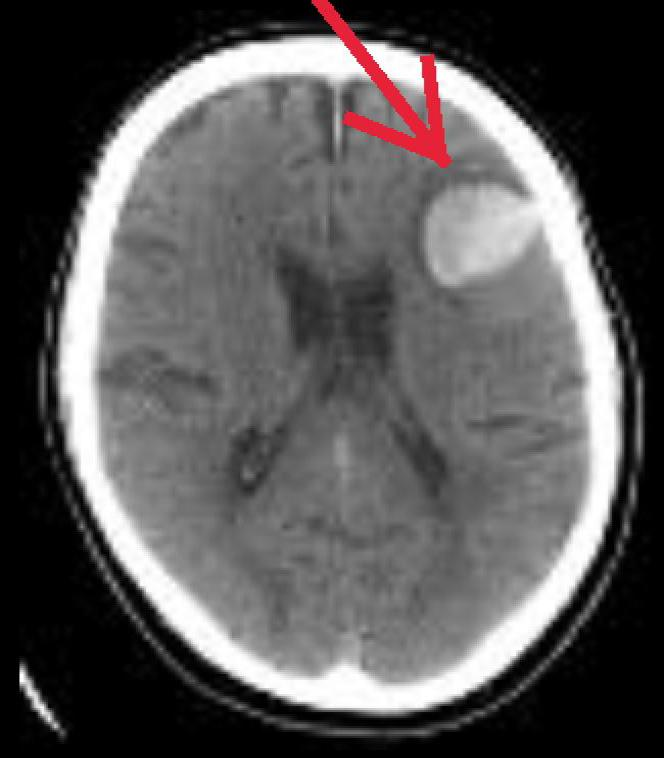
\includegraphics[width=6cm]{"Images/Chapter1/intraparenchymal.JPG"}} & 
\parbox[c][7cm][c]{7cm}{\centering 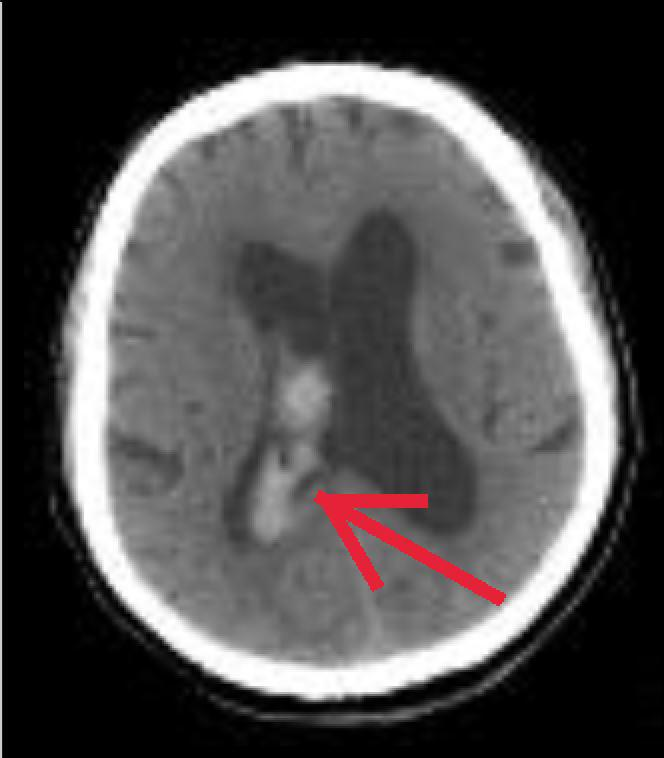
\includegraphics[width=6cm]{Images/Chapter1/intraventricular.JPG}} & 
\parbox[c][7cm][c]{7cm}{\centering 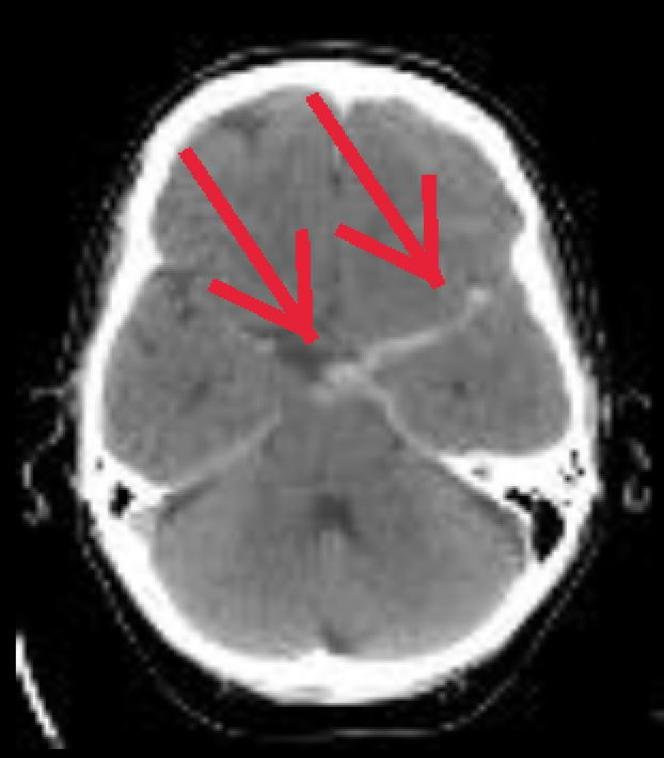
\includegraphics[width=6cm]{Images/Chapter1/subarachnoid.JPG}} & 
\parbox[c][7cm][c]{7cm}{\centering 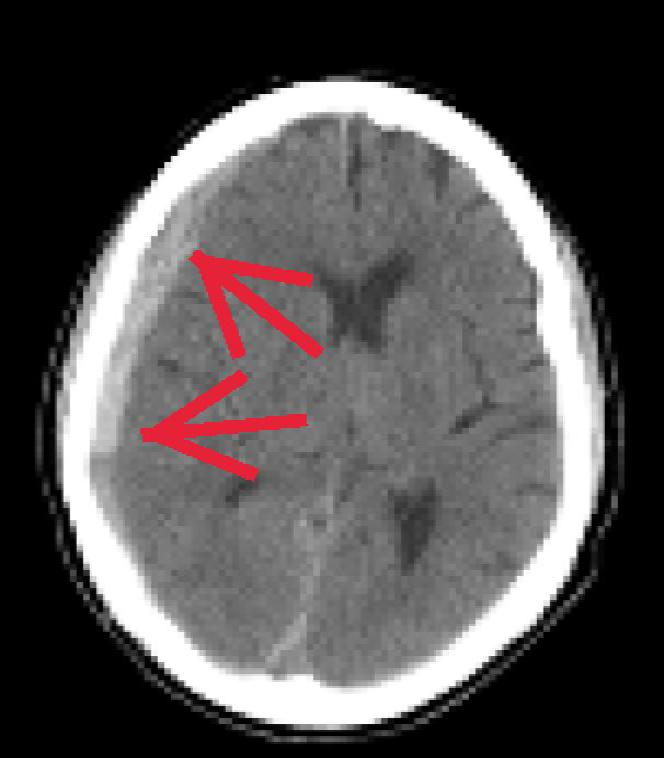
\includegraphics[width=6cm]{Images/Chapter1/subdural.JPG}} & 
\parbox[c][7cm][c]{7cm}{\centering 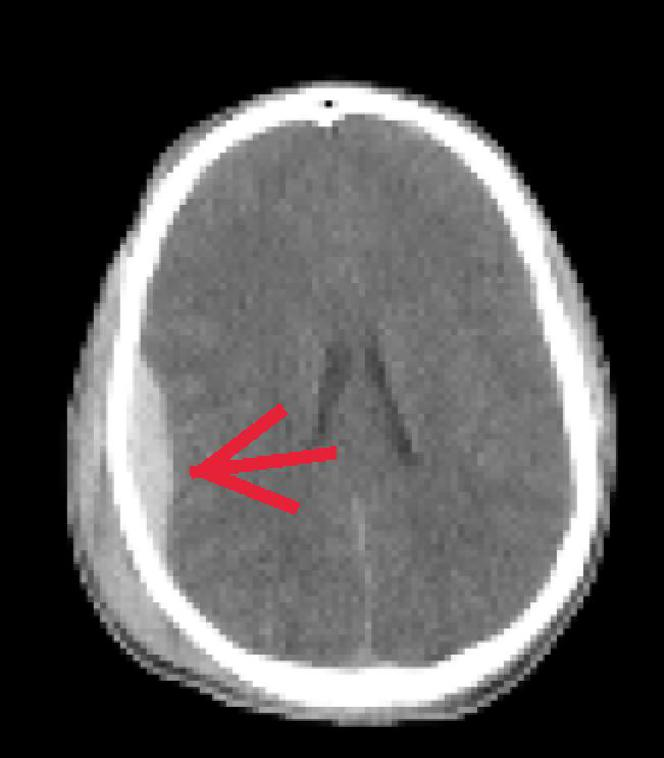
\includegraphics[width=6cm]{Images/Chapter1/Epidural.JPG}} \\ \hline
\textbf{زمینه‌ها} & فشار خون بالا، ضربه، ناهنجاری‌های شریانی-وریدی، تومور، و غیره & می‌تواند با خونریزی‌های درون‌مغزی و زیرعنکبوتیه همراه باشد & پارگی آنوریسم یا ناهنجاری‌های شریانی-وریدی یا ضربه & ضربه & ضربه یا پس از جراحی \\ \hline
\textbf{علت وقوع} & شریانی یا وریدی & شریانی یا وریدی & عمدتاً شریانی & وریدی (وریدهای پل‌زن) & شریانی \\ \hline
\textbf{شکل} & معمولاً گرد & مطابق با شکل بطن & در امتداد شیارها و شکاف‌ها & هلالی & عدسی‌شکل \\ \hline
\textbf{علائم بالینی} & حاد (شروع ناگهانی سردرد، حالت تهوع، استفراغ) & حاد (شروع ناگهانی سردرد، حالت تهوع، استفراغ) & حاد (بدترین سردرد زندگی) & ممکن است تدریجی باشد (بدتر شدن سردرد) & حاد (شکستگی جمجمه و تغییر وضعیت ذهنی) \\ \hline
\end{tabular}}
\caption{انواع زیرگروه‌های خونریزی درون‌جمجمه‌ای
\cite{rsna_hemorrhage_detection_kaggle}}
\label{table: subtype}
\end{table}

  
\section{روش‌های مرسوم در تشخیص خونریزی درون‌جمجمه‌ای}

در حال حاضر تصاویر سی‌تی‌اسکن، به‌عنوان استاندارد اصلی و غیرتهاجمی
\LTRfootnote{Non-invasive}
برای تشخیص خونریزی‌ درون‌جمجمه‌ای است. سی‌تی‌اسکن یک نوع تصویر پرتونگاری
\LTRfootnote{Radiography}
سه‌بعدی است که متشکل از تصاویر دوبعدی از اندام بدن است. روش عمومی پردازش تصاویر سی‌تی‌اسکن به‌صورت دستی انجام می‌پذیرد که به‌موجب آن متخصصین پرتونگاری
\LTRfootnote{Radiology}
 و پزشکی، با بررسی برش‌های
\LTRfootnote{ُSlice}
سی‌تی‌اسکن را به‌صورت مجزا بررسی می‌کنند و مناطق خونریزی را تشخیص می‌دهند. این فرایند به دلیل وابستگی به تخصص و تجربه فردی، شرایط محیطی و فشار کاری، زمان‌بر و مستعد خطا است. \cite{arbabshirani2018advanced,grewal2018radnet,ye2019precise,chilamkurthy2018deep,kuo2019expert}.
فرایند بررسی دستی تصاویر سی‌تی‌اسکن، زمان‌بر بوده و به‌شدت به دردسترس‌بودن پرتونگار‌های 
\LTRfootnote{Radiologist}
باتجربه بستگی دارد \cite{burduja2020accurate}.
 در شرایط اضطراری، خصوصا در مراکز فوریت‌های پزشکی، زمانی که برای پردازش برش‌های سی‌تی‌اسکن صرف می‌شود، می‌تواند به طور قابل‌توجهی در نتایج درمان بیمارها تأثیر بگذارد؛ این مسئله در مواردی از اهمیت بیشتری برخوردار می‌شود که درمان بیمار نیازمند مداخله فوری گروه پزشکی است \cite{chilamkurthy2018deep}. نکته حائز اهمیت در روش معمول برای بررسی تصاویر سی‌تی‌اسکن در مراکز پزشکی این است که بررسی اولیه تصاویر، توسط پزشکان و پرتونگار‌هایی با تجربه کمتر انجام می‌شود و در مراحل بعدی این تصاویر توسط متخصصینی با تجربه بیشتر بررسی می‌شود. تعدادی از مطالعات نشان داده‌اند که در روش مذکور،‌ بین پزشکان و پرتونگار‌هایی که در مرحله اول تصاویر را بررسی می‌کنند و پزشکان و پرتونگار‌هایی که در ادامه این تصاویر را بررسی می‌کنند،‌ اختلاف‌نظر وجود دارد که این مسئله می‌تواند منجر به عواقب جبران‌ناپذیر گردد
\cite{ye2019precise, alfaro1995accuracy, lal2000clinical, erly2002radiology, strub2007overnight}.
   احتمال خطای انسانی در بررسی دستی تصاویر پیچیده و سه‌بعدی سی‌تی‌اسکن، از دیگر نقاط ضعف روش معمول پردازش این تصاویر است، به‌ویژه در محیط‌های شلوغ و پرتنش که پرتونگار‌ها ممکن است تحت فشار زیاد باشند \cite{ye2019precise}.
   
\section{روش‌های رایانه‌ای در پردازش تصاویر پزشکی}
اهمیت مسئله خونریزی درون‌جمجمه‌ای و چالش‌های مرتبط با آن در بخش قبل مورد بررسی قرار گرفت، روش‌های مبتنی‌ بر پردازش رایانه‌ای
\LTRfootnote{Computer}
تصاویر پزشکی، می‌تواند یک راه‌حل مناسب برای رفع نقاط ضعف روش کنونی بررسی تصاویر پزشکی باشد
\cite{grewal2018radnet, arbabshirani2018advanced, ye2019precise, lee2019explainable, chang2018hybrid, chilamkurthy2018deep, titano2018automated, kuo2019expert}.
 ابزارهای خودکار برای تشخیص و کمیت‌سنجی خونریزی، از پیشرفت‌های روش‌های یادگیری ماشین 
\LTRfootnote{Machine Learning}
و یادگیری عمیق
\LTRfootnote{Deep Learning}
 و سامانه‌های
 \LTRfootnote{System}
  تشخیص به کمک رایانه 
 \LTRfootnote{Computer-aided Diagnosis}
 استفاده می‌کنند تا تجزیه‌وتحلیل سریع و دقیقی از تصاویر سی‌تی‌اسکن ارائه دهند. با خودکارسازی تشخیص خونریزی درون‌جمجمه‌ای و استفاده از آنها به‌صورت نظر ثانویه
  \LTRfootnote{ُSecond Opinion}
 ، این سامانه‌ها می‌توانند بار کاری پرتونگار‌ها را کاهش دهند، دقت تشخیص را افزایش دهند از اشتباهات متخصصین جلوگیری کنند، زمان تشخیص را به حداقل برسانند، بعضی از هزینه‌های فرایند درمان را به علت کاهش دخالت انسانی کاهش دهند و به‌صورت کلی فرایند تشخیص را بهبود ببخشند که این موارد به بهبود نتایج بیماران منجر خواهد شد. بااین‌حال، ضمن اینکه سامانه‌های تشخیص به کمک رایانه نویدبخش هستند؛ اما امکان خطا در آنها وجود دارد که می‌تواند تصمیم‌گیری بالینی را با مشکلاتی روبرو کند؛ بنابراین، ادغام این ابزارها در عمل باید با دقت انجام شود \cite{titano2018automated}.
 
 
 
 \section{مجموعه‌داده‌ها}
 
 
 در سال‌های اخیر، مجموعه‌داده‌های متعددی برای پشتیبانی از توسعه مدل‌های
 \LTRfootnote{Model}
  یادگیری عمیق در حوزه تصویربرداری پزشکی، به‌ویژه برای طبقه‌بندی خونریزی درون‌جمجمه‌ای ایجاد شده‌اند. در ادامه به بررسی برخی از مهم‌ترین مجموعه‌داده‌هایی که در این حوزه مورد استفاده قرار گرفته‌اند، می‌پردازیم.
 
 \subsection{مجموعه‌داده‌ی انجمن پرتوشناسی آمریکای شمالی
  \lr{(RSNA)}}
 مجموعه‌داده‌ی 
 \lr{RSNA Intracranial Hemorrhage Detection}\cite{rsna_hemorrhage_detection_kaggle,rsna_kaggle}
  که برای چالش یادگیری ماشین سال ۲۰۱۹ انجمن پرتونگاری آمریکای شمالی جمع‌آوری شده است، یکی از منابع برجسته در زمینه طبقه‌بندی خونریزی درون‌جمجمه‌ای محسوب می‌شود. این مجموعه‌داده،از چند مرکز پرتونگاری جمع آوری شده است که سه مؤسسه دانشگاه استنفورد در ایالات متحده، دانشگاه فدرال سائو پائولو در برزیل و بیمارستان دانشگاه توماس جفرسون در ایالات متحده شامل آنها می‌باشد. این مجموعه شامل تصویر سی‌تی‌اسکن مغزی ۲۵۳۱۲ بیمار است که از این میان، ۸۸۸۹ بیمار دارای انواع مختلف خونریزی درون‌جمجمه‌ای هستند. تصاویر سی‌تی‌اسکن درون این مجموعه‌داده درسطح برش،‌ حاشیه‌نویسی 
   \LTRfootnote{Annotation}
 شده‌اند.  تصاویر سی‌تی‌اسکن در این مجموعه‌داده به فرمت
  \lr{DICOM}
  \LTRfootnote{Digital Imaging and Communications in Medicine}
   ارائه شده‌اند که استانداردی برای تصویربرداری پزشکی است. این مجموعه‌داده به‌طور گسترده‌ای در طبقه‌بندی انواع خونریزی مورد استفاده قرار گرفته و به‌عنوان منبعی بنیادی برای آموزش و اعتبارسنجی مدل‌های یادگیری ماشین که به طبقه‌بندی خونریزی درون‌جمجمه‌ای تبدیل شده است.
 
 \subsection{مجموعه‌داده‌ی \lr{MosMed}}
 مجموعه‌داده‌ی
  \lr{MosMed}\cite{medmos_khoruzhaya2024expanded}،
  یک مجموعه‌داده خونریزی درون‌جمجمه‌ای می‌باشد که در روسیه جمع‌آوری شده است. این مجموعه‌داده به‌طور خاص برای تسهیل توسعه سیستم‌های هوش مصنوعی به‌منظور تشخصی و طبقه‌بندی خونریزی درون‌جمجمه‌ای طراحی شده است. این مجموعه شامل سی‌تی‌اسکن مغزی ۸۰۰ بیمار است که 400 بیمار دارای خونریزی درون‌جمجمه‌ای هستند. این مجموعه داده درسطح بیمار حاشیه‌نویسی شده است و تصاویر آن به صورت فایل‌های 
  \lr{DICOM}
  دردسترس قرار دارد.
 
 \subsection{مجموعه‌داده‌ی \lr{CQ500}}
 مجموعه‌داده‌ی
  \lr{CQ500}\cite{cq500_chilamkurthy2018development}
  ، یک مجموعه‌داده مهم است که از چند مرکز متفاوت شامل پنج مرکز مختلف در هند می‌باشد. این مجموعه‌داده خاوی ۴۹۱ سی‌تی‌اسکن سر است که برای انواع خونریزی‌های درون‌جمجمه‌ای درسطح بیمار حاشیه‌گذاری شده‌اند. تصاویر سی‌تی‌اسکن در این مجموعه‌داده به صورت فایل
   \lr{DICOM}
    ارائه شده.
 \subsection{مجموعه‌داده‌ی \lr{PHE-SICH-CT-IDS}}
 مجموعه‌داده‌ی 
 \lr{PHE-SICH-CT-IDS}\cite{PHE_ma2024phe}
 ، اگرچه به‌طور خاص برای خونریزی درون‌جمجمه‌ای جمع‌آوری نشده است، اما به دلیل تمرکز آن بر وظایف طبقه‌بندی، تشخیص و قطعه‌بندی مرتبط به 
 \lr{Perihematomal Edema}
  در خونریزی‌ درون‌جمجمه‌ای قابل توجه است. این مجموعه‌داده‌ از بیمارستان 
  \lr{Shengjing}
  در چین جمع‌آوری شده است که 
   شامل تصویر سی‌تی‌اسکن 120 بیمار است که تمامی آنها خونریزی درون‌جمجمه‌ای دارند و حاشیه‌نویسی آنها در سطج برش انجام شده است. تصاویر سی‌تی‌اسکن در این مجموعه داده به صورت فایل‌های 
   \lr{NIFTI},
   \lr{JPG} و
   \lr{PNG}
   ارائه شده است. مجموعه‌داده‌ی 
   \lr{PHE-SICH-CT-IDS}
    منبعی ارزشمند برای توسعه مدل‌های یادگیری عمیق که هدف آن‌ها طبقه‌بندی، تشخیص یا قطعه‌بندی می‌باشد، است. در
   \autoref{fig:ch1-phe-sample}
 چند برش از تصاویر مجموعه داده 
 \lr{PHE-SICH-CT-IDS}
 است، همانطور که در این تصویر مشخص است،‌ در اطراف ضایعه خونریزی،‌ یک حاشیه تیره‌تر وجود داره که به آن 
 \lr{Edma}
 گفته می‌شود و این ضایعه قطعه‌بندی شده است؛ همچنین این مجموعه‌داده حاشیه‌نویسی مناسب برای وظیفه تشخیص را نیز دارد.
 \begin{figure}[H]
 \centering
 \includegraphics[width=1.0\linewidth]{"Images/Chapter1/PHE sample"}
 \caption{چند نمونه تصویر از مجموعه‌داده 
 \lr{PHE-SICH-CT-IDS}}
 \label{fig:ch1-phe-sample}
 \end{figure}
 
 \subsection{مجموعه‌داده‌ی \lr{PhysioNet}}
 مجموعه‌داده‌ی خونریزی درون‌جمجمه‌ای 
 \lr{PhysioNet}\cite{physionet_hssayeni2020intracranial}،
 مجموعه‌داده‌ای می‌باشد که در ادامه این مطالعه از آن استفاده شده است. این مجموعه داده
 از بیمارستان
 \lr{Al Hilla}
 در عراق جمع‌آوری شده است و شامل 82 تصویر سی‌تی‌اسکن از بیماران است که 36 نفر از آنها دارای خونریزی درون جمجمه‌ای می‌باشند.
   این مجموعه داده، شامل حاشیه‌نویسی‌های مناسب برای وظایف طبقه‌بندی و قطعه‌بندی است که آن را به تنها مجموعه‌داده با دسترسی عمومی تبدیل می‌کند که امکان قطعه‌بندی خونریزی درون‌جمجمه‌ای را فراهم می‌کند. جزییات بیشتر درمورد این دیتاست در 
   \autoref{}
 توضیح داده شده است.
 تصویر
 \autoref{fig:ch1-physionet-sample}
 چند نمونه از برش‌های خونریزی درون این مجموعه‌داده را مشخص می‌کند.
 \begin{figure}[H]
 \centering
 \includegraphics[width=1.0\linewidth]{"Images/Chapter1/physionet sample"}
 \caption{چند نمونه تصویر از مجموعه داده
 \lr{PhysioNet}}
 \label{fig:ch1-physionet-sample}
 \end{figure}
 
 
 \section{تحقیقات اخیر در زمینه یادگیری ماشین}
 
 در سال‌های اخیر، یادگیری عمیق پیشرفت‌های قابل‌توجهی در زمینه طبقه‌بندی و قطعه‌بندی خونریزی درون‌جمجمه‌ای داشته است و مطالعات متعددی به بررسی این موضوع پرداخته‌اند. این مدل‌ها نه تنها از نظر نوآوری فنی قابل‌توجه هستند، بلکه پتانسیل بالای آنها می‌تواند باعث استفاده از آنها در سیستم‌های تشخیص و درمان بیمارستان‌ها بشود که می‌تواند بهبود عملکرد کادر درمان، کاهش هزینه‌ها و زمان تشخیص و افزایش دقت در طبقه‌بندی خونریزی درون‌جمجمه‌ای را به همراه داشته باشد. برخی از این مطالعات، از جمله تحقیقات
  \lr{Titano}\cite{titano2018automated}, \lr{Arbabshirani}\cite{arbabshirani2018advanced} و \lr{Kuo}\cite{kuo2019expert}،
و همکارانشان مدل‌های پیشنهادی خود را در محیط‌های بیمارستانی آزمایش کرده‌اند و نتایج آن‌ها نشان داده است که این سیستم‌ها می‌توانند به‌طور مؤثری در بهبود نتایج درمان برای بیماران نقش داشته باشد. به‌طور خاص، \lr{Titano} و همکاران یک سیستم یادگیری عمیق خودکار با دقت \(87\%\) و حساسیت \(94\%\) معرفی کرده‌اند که عملکرد آن با کارشناسان انسانی مقایسه شده و در محیط‌های بالینی به کار گرفته شده است. همچنین، \lr{Kuo} و همکاران یک شبکه عصبی پیچشی برای طبقه‌بندی خونریزی حاد درون‌جمجمه‌ای با دقت \(99\%\) و \lr{AUC} برابر با
 \(99\%\)
توسعه داده‌اند که نشان‌دهنده قابلیت اطمینان بالا در شرایط بالینی است. سایر مطالعات، مانند
 \lr{Chang}\cite{chang2018hybrid}
  و
   \lr{Chilamkurthy}\cite{chilamkurthy2018deep}
    نیز نتایج قابل‌توجهی در زمینه طبقه‌بندی خونریزی‌ها با استفاده از مدل‌های یادگیری عمیق ارائه کرده‌اند.
 
 \lr{Neethi}\cite{neethi2022stroke} و همکاران 
 مروری بر روش‌های مختلف یادگیری عمیق انجام داده‌اند که از مجموعه‌داده‌های مختلفی از جمله \lr{PhysioNet} و مجموعه‌داده \lr{RSNA} استفاده کردند. آنها از مجموعه‌داده \lr{RSN } که شامل 25312 تصویر سی‌تی‌اسکن از بیماران است، برای آموزش مدل‌های یادگیری عمیق بهره بردند و عملکرد آن را بر روی مجموعه‌داده \lr{PhysioNet} ارزیابی کردند. آن‌ها با استفاده از مدل \lr{ResNet50-V2} بر روی مجموعه‌داده \lr{PhysioNet} به
  \lr{‎Recall}‎ \(76\%\) و \lr{F1 Score}
   برابر با 
   \(67\%\) 
   دست یافتند که این نتایج به صورت برش‌محور
   \LTRfootnote{Slice-wise}
   گزارش شده است.
 در میان کارهایی که روی مجموعه‌داده \lr{PhysioNet} انجام شده است،
  \lr{Kyung}\cite{kyung2022improved}
و همکاران
شبکه‌ای به نام 
\lr{SMART-Net} 
را پیشنهاد کردند که به کمک روش انتقال یادگیری
\LTRfootnote{Transfer Learning}
توانسته‌اند به \lr{F1 Score} برابر با
 \(84\%\)
 و 
 \lr{Sensitivity}
 برابر با 
  \(97\%\)
  و 
  \lr{Specificity}
  برابر با
  \(74\%\)
  بیمارمحور 
  \LTRfootnote{Patient-wise}
   دست یابند.
 
 
 \subsection{نقاط ضعف موجود در پژوهش‌های گذشته}
 
 
 
 
 با وجود پیشرفت‌های قابل‌توجه در مدل‌های یادگیری عمیق، هنوز چالش‌هایی در تفسیرپذیری مدل‌های شبکه عصبی وجود دارد که می‌توان از آن به عنوان یکی از نقاط ضعف ادبیات موجود در این زمینه دانست زیرا تفسیرپذیر بودن یک سیستم هوش مصنوعی، یکی از معیارهای اساسی برای متخصصین حوزه پزشکی است تا از این ابزار استفاده کنند. از دیگر نقاط ضعف در ادبیات خونریزی درون‌جمجمه‌ای، دردسترس نبودن مجموعه‌داده‌های بزرگ با حاشیه‌نویسی مناسب و مجموعه‌داده‌های مربوط به بیمارستان‌ها و دستگاه‌های موجود در ایران است؛ وجود یک مجموعه‌داده با ابعاد مناسب از دستگاه‌های موجود در ایران، می‌تواند مسیر توسعه یک سیستم هوش مصنوعی در زمینه خونریزی‌درون جمجمه‌ای را در ایران وجود هموار سازد. از دیگر نقاط ضعف موجود در ادبیات موجود در این مسئله، استفاده از شبکه‌هایی با ابعاد بسیار بزرگ توسط محققین می‌باشد که نیازمند پردازشگر‌هایی با هزینه بیشتر هستند. از مهم‌ترین مشکلات موجود در تحقیقات گذشته، توجه نکرده به بیمارمحور بودن داده‌ها هنگام تفکیک آنها به زیرمجموعه‌های آموزش و ارزیابی اشاره کرد که درنتیجه‌ آن برش‌هایی از یک بیمار که شباهت بسیار زیادی به یکدیگر دارند، در زیرمجموعه‌های آموزش و ارزیابی قرار گیرد که درنتیجه آن همبستگی بین این دو مجموعه داده زیاد خواهد شد.
استفاده نکردن از روش مرسوم
\lr{K-Fold-Cross-Validation}، 
یکی دیگر از معایب موجود در تحقیقات گذشته است که به‌موجب آن، تعمیم‌پذیری مدل بدست آمده از این تحقیقات محل ابهام می‌باشد.
به عنوان یکی از اشکالات مهم در ادبیات موجود، عدم ارائه معیارهای مناسب و کافی برای ارزیابی عملکرد مدل‌های یادگیری ماشین است که در نتیجه آن، نتایج بدست آمده از شفافیت کافی برخوردار نیست.
 \subsection{دستاوردهای ما و نحوه حل مشکلات گذشته}
 در این پژوهش تلاش شده تا در گام نخست یک روش دو مرحله‌ای شامل یک مدل طبقه‌بندی و یک مدل قطعه‌بندی که به صورت متوالی استفاده می‌شوند توسعه داده شود که این روش،  موجب بهبود عملکرد مدل‌های پردازش تصویر در قطعه‌بندی شده است؛ نکته حائز اهمیت در این روش این است که با کاهش امکان ایجاد 
 \lr{False Positive}
 در پیش‌بینی‌های مدل قطعه‌بندی، باعث بهبود عملکرد مدل‌های قطعه‌بندی خواهد شد.
  در گام بعدی یک پس‌پردازش
 \LTRfootnote{Post-process}
  در لایه تصمیم‌گیری توسعه داده شده است که این پس‌پردازش نیز موجب بهبود عملکرد مدل طبقه‌بندی شده است.
 در انتها با استفاده از انواع معیارهای موجود، آموزش مدل با استفاده از روش
 \lr{5-Fold-Cross-Validation}،
  طراحی یک ضابطه تصمیم‌گیری
 \LTRfootnote{Decision Policy}
 
  و استفاده از روش‌هایی برای تفسیر‌پذیر کردن مدل، امکان تحلیل جامع از عملکرد مدل فراهم شده است.

\chapter{روش‌ها و مجموعه‌داده}
\label{dataset}
\section{بررسی آماری مجموعه‌داده}

در این پژوهش از مجموعه‌داده
\lr{PhysioNet}\cite{physionet_hssayeni2020intracranial,hssayeni2020computed}
استفاده شده است که شامل حاشیه‌نویسی برای وظیفه طبقه‌بندی و قطعه‌بندی است. این مجموعه‌داده  شامل مجموعه‌ای از سی‌تی‌اسکن‌های مغزی است که به‌صورت عمومی در دسترس است.
\begin{figure}[h]
\centering
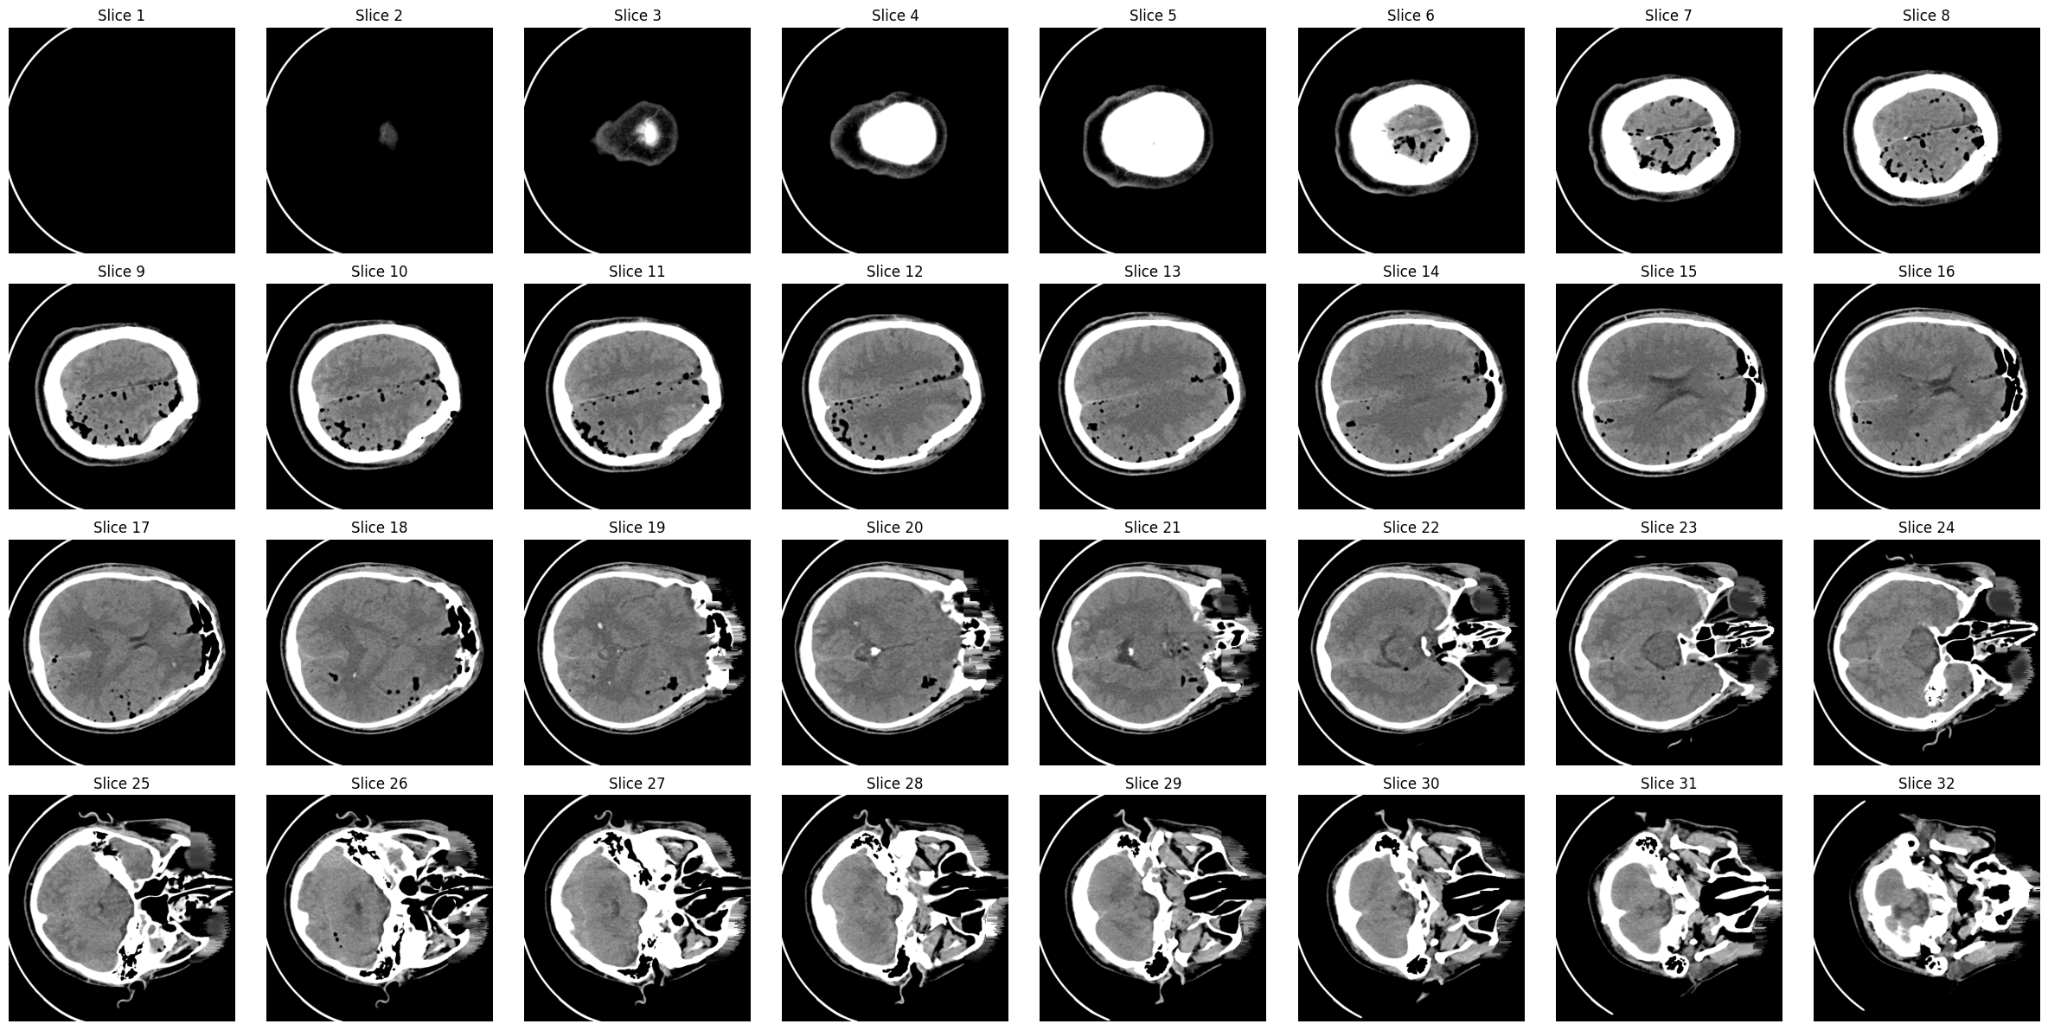
\includegraphics[width=1.0\linewidth]{Images/Chapter2/3d}
\caption{یک نمونه کامل از تصاویر سی‌تی‌اسکن}
\label{fig:ct2-3d}
\end{figure}


همانطور که در 
\autoref{fig:ct2-3d}
نمایش‌داده‌شده است، سی‌تی‌اسکن یک نوع تصویر سه‌بعدی است که از برش‌های دوبعدی تشکیل شده است. 
\autoref{fig:read-ct}
 نشان می‌دهد که
 باتوجه‌‌به جهت بررسی برش‌های سی‌تی‌اسکن، این تصاویر به سه دسته 
 \lr{Axial}, \lr{Sagital} و \lr{Coronal}
 تقسیم می‌شوند.
\begin{figure}[h]
\centering
\includegraphics[width=1.0\linewidth]{"Images/Chapter2/read CT"}
\caption{خوانش‌های متفاوت از تصاویر سی‌تی‌اسکن
\cite{kaggleCTScansDICOM}}
\label{fig:read-ct}
\end{figure}
 
مجموعه‌داده 
\lr{PhysioNet}
 شامل 82 سی‌تی‌اسکن با برش‌‌های 
\lr{Axial}
است که بین فوریه و اوت 2018 از بیمارستان آموزشی 
\lr{Al Hilla }
 در عراق جمع‌آوری شده است. این اسکن‌ها شامل طیف وسیعی از بیماران هستند که از یک روز تا 72 سال سن دارند و میانگین سن آنها 
 $27.8 \pm 19.5$
 سال است. تنوع سنی این مجموعه‌داده بر مقیاس، شکل جمجمه و بافت مغز در سی‌تی‌اسکن تأثیر می‌گذارد، عاملی که می‌تواند عملکرد مدل‌های یادگیری عمیق برای تشخیص و قطعه‌بندی خونریزی درون جمجمه‌ای را تحت‌تأثیر قرار دهد. توزیع جنسیت در این مجموعه‌داده به‌گونه‌ای است که 56\%  بیماران مرد و 44\% آنها زن هستند.
82 بیماری که در این مجموعه‌داده وجود دارد که 7 مورد از آنها طی فرایند حاشیه‌نویسی گم شده‌اند و از بین 75 بیمار موجود، 36 نفر دارای خونریزی درون‌جمجمه‌ای تشخیص داده شدند.
\autoref{fig:ch2-slice-number}
نمودار تعداد برش‌های هر بیمار در این مجموعه‌داده است؛ تصاویر سی‌تی‌اسکن موجود در این مجموعه‌داده،  به به‌صورت متوسط شامل 34 برش با ضخامت برش 5 میلی‌متر دارند و در مجموع 2814 برش در این مجموعه‌داده وجود دارد. 
\begin{figure}[h]
\centering
\includegraphics[width=1.0\linewidth]{"Images/Chapter2/Slice number"}
\caption{‌تعداد برش‌های بیماران بر اساس شناسه اختصاصی آنها}
\label{fig:ch2-slice-number}
\end{figure}

بااین‌حال، این مجموعه‌داده به دلیل عدم توازن در سطح برش شناخته می‌شود، زیرا تنها 318 برش دارای خونریزی هستند درحالی‌که  بقیه 2496 برش سالم هستند. در این مجموعه‌داده، 24 برش شامل زیرگروه
 \lr{IVH}،
  73 برش شامل زیرگروه
 \lr{CPH}، 
  18 برش شامل زیرگروه
 \lr{SDH}،
173 برش شامل زیرگروه
 \lr{EDH} 
 و 56 برش شامل زیرگروه 
 \lr{SDH}
هستند. باتوجه‌به تفاوت شکل انواع زیرگروه‌های خونریزی و محل وقوع آنها، این ارقام نشان‌دهنده عدم وجود تعداد برش کافی برای بعضی از انواع زیرگروه‌ها است.
در این مجموعه‌داده، برش‌های سی‌تی‌اسکن توسط دو پرتوشناس بررسی شده است و هر برش سی‌تی‌اسکن از نظر وجود خونریزی یا شکستگی توسط آنها بررسی و برچسب‌گذاری شده است. در ادامه سی‌تی‌اسکن‌های دو بیمار، به علت کیفیت ضعیف تصاویر و به توصیه پرتوشناس‌ها حذف شدند\cite{kyung2022improved}.

\autoref{fig: ch2-distribution}
نمودارهای توزیع بیمارمحور و برش‌محور مجموعه‌داده را نمایش می‌دهد؛ همانطور که از ‎\autoref{fig: ch2-patient distrbiution}‎ مشخص است در بررسی بیمار‌محور این مجموعه‌داده، عدم توازن دیده نمی‌شود؛ اما در بررسی برش‌محور، همانطور که در ‎\autoref{fig: ch2-slice distribution}‎ 
مشخص است، عدم توازن شدیدی در تعداد برش‌های دارای خونریزی وجود دارد که این مسئله، آموزش مدل‌های شبکه عصبی را با چالش مواجه می‌کند.
 \begin{figure}[ht]
		\centering % <-- added
		\begin{subfigure}{0.45\textwidth}
			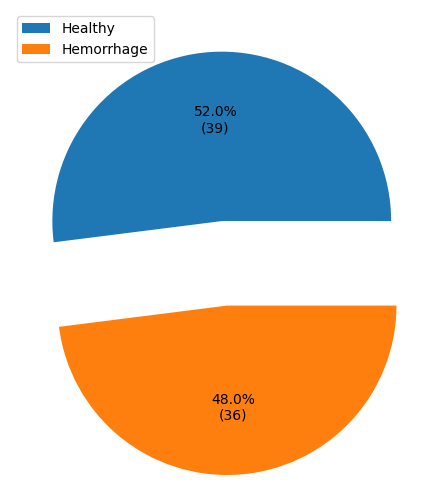
\includegraphics[width=\linewidth]{Images/Chapter2/patient distrbiution.png}
			\caption{}
			\label{fig: ch2-patient distrbiution}
		\end{subfigure}\hfil % <-- added
		\begin{subfigure}{0.45\textwidth}
			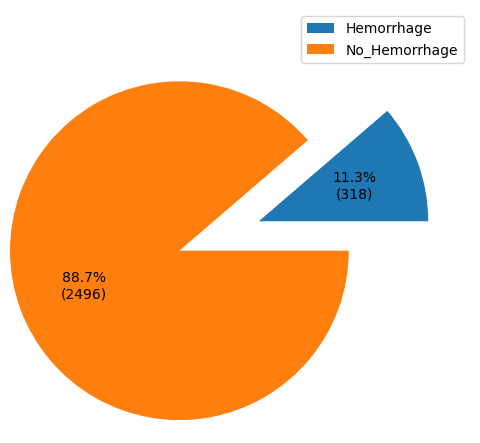
\includegraphics[width=\linewidth,]{Images/Chapter2/slice distribution.png}
			\caption{}
			\label{fig: ch2-slice distribution}
		\end{subfigure}
		\caption{توزیع بیماران و برش‌ها در مجموعه‌داده 
		\lr{PhysioNet}}
		\label{fig: ch2-distribution}
\end{figure} 

 علاوه‌بر وجود عدم توازن در حالت برش‌محور، عدم توازن شدیدی در قطعه‌بندی نواحی دارای خونریزی نسبت به نواحی سالم در برش‌های دارای خونریزی وجود دارد که به‌موجب آن در یک تصویر با ابعاد
$512\times512$،
به‌صورت میانگین نزدیک به 2000 پیکسل
\LTRfootnote{Pixel}
دارای خونریزی درون‌جمجمه‌ای وجود دارد که این مسئله، آموزش مدل‌های شبکه عصبی را به‌منظور وظیفه قطعه‌بندی با چالش بسیار جدی مواجه می‌کند. 
\autoref{fig: ch2-slice hist}
نشان‌دهنده توزیع نرمال‌شده 
\LTRfootnote{Normalized}
مقدار پیکسل‌های برش‌های سالم و برش‌های دارای خونریزی است، باتوجه‌به
\autoref{fig: ch2-slice hist whole}، 
اکثر پیکسل‌های تصاویر مقداری نزدیک به 
$-1000$
و نقطه بیشینه محلی بعدی برای این نمودار توزیع، در نزدیک مقادیر 30 است که این مقادیر به نسبت پیکسل‌ها با مقادیر نزدیک به 
$-1000$
خیلی کمتر است.


 \begin{figure}[ht]
		\centering % <-- added
		\begin{subfigure}{0.45\textwidth}
			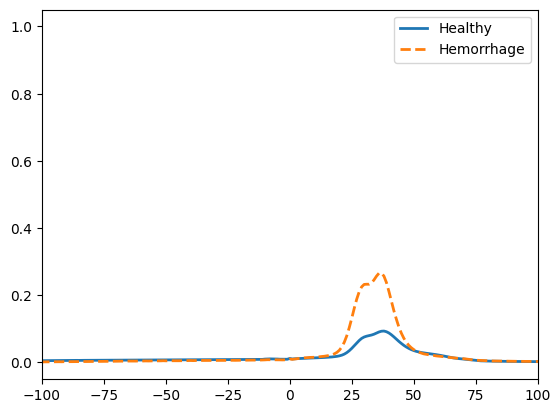
\includegraphics[width=\linewidth]{Images/Chapter2/Pixel histogram.png}
			\caption{}
			\label{fig: ch2-slice hist lim}
		\end{subfigure}\hfil % <-- added
		\begin{subfigure}{0.45\textwidth}
			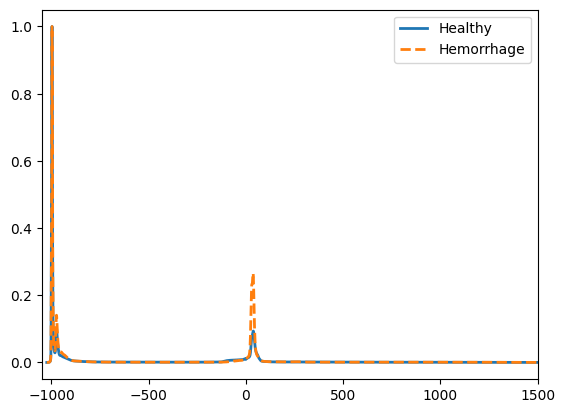
\includegraphics[width=\linewidth,]{Images/Chapter2/Pixel histogram lim.png}
			\caption{}
			\label{fig: ch2-slice hist whole}
		\end{subfigure}
			\caption{توزیع پیکسلی برش‌ها برای برش‌های دارای خونریزی در مقال برش‌های سالم}
		\label{fig: ch2-slice hist}
\end{figure} 

\autoref{fig:ch2-pixel-hist-ich-vs-healthy}
نمایش‌دهنده توزیع پیکسل‌های دارای خونریزی و تمام پیکسل‌های تصاویر پرتونگاری است که در محدوده بین 
$-100$
تا 
$100$
واقع شده است و نسبت به مقادیر همین بازه نرمال گشته است. همانطور که از این دو نمودار مشخص است، مقادیر مربوط به ضایعه خونریزی،‌ به‌اندازه کمی از مقادیر بقیه بافت‌های مغز روشن‌تر است؛ اما همپوشانی این دو نمودار نشان می‌دهد که تشخیص خونریزی درون‌جمجمه‌ای تنها با استفاده از مقدار پیکسلی آن بسیار دشوار است و نیاز هست تا از شبکه‌هایی استفاده شود تا به اشکال موجود در تصویر نیز حساسیت داشته باشند.


\begin{figure}[h]
\centering
\includegraphics[width=1.0\linewidth]{"Images/Chapter2/pixel hist ich vs healthy"}
\caption{توزیع نرمال‌شده پیکسل‌های دارای خونریزی در مقابل تمام پیکسل‌های تصاویر}
\label{fig:ch2-pixel-hist-ich-vs-healthy}
\end{figure}


\autoref{fig:ch2-slice-number}
توزیع خونریزی درون‌جمجمه‌ای را بر اساس شماره برش در تصویر سی‌تی‌اسکن نشان می‌دهد که بر اساس آن مشخص است به‌ازای بعضی از شماره برش‌ها، خونریزی درون‌جمجمه‌ای وجود ندارد و این برش‌ها از اهمیت کمتری برای مدل‌های یادگیری ماشین برخوردار هستند.

\begin{figure}[h]
\centering
\includegraphics[width=1.0\linewidth]{"Images/Chapter2/slice hist"}
\caption{توزیع خونریزی بر اساس برش‌ها}
\label{fig:ch2-slice-hist}
\end{figure}


باتوجه‌به مطالبی که در این بخش مطرح شد، ‌می‌توان نتیجه‌ گرفت که مجموعه‌داده
 \lr{PhysioNet}،
به‌عنوان تنها مجموعه‌داده عمومی قطعه‌بندی خونریزی درون‌جمجمه‌ای، می‌تواند یک مجموعه‌داده معیار برای بررسی عملکرد مدل‌های پردازش تصویر باشد. 

\autoref{fig:ch3-wholeheatmap}
نمایش پراکندگی مکانی خونریزی درون‌جمجمه‌ای را نشان می‌دهد که در مجموعه‌داده
\lr{PysioNet}
وجود دارد. این پراکندگی نشان می‌دهد که خونریزی درون‌جمجمه‌ای تنها در قسمت‌های خاصی از برش‌های سی‌تی‌اسکن اتفاق می‌افتد و از طرف دیگر احتمال وجود خونریزی در اطراف جمجمه و ناحیه شقیقه،‌ بیشتر از پیشانی و پشت سر است.
\autoref{fig:heatmaps}
نمایش زیرمجموعه‌های متفاوتی است که در فرایند آموزش و ارزیابی مدل دخیل بوده‌اند. باید توجه داشت که در این تصویر، نقشه پراکندگی مربوط‌ به هر 
\lr{Fold}
نشان‌دهنده زیرمجموعه آموزش به‌ازای آن 
\lr{Fold}
است.  
\begin{figure}[h]
\centering
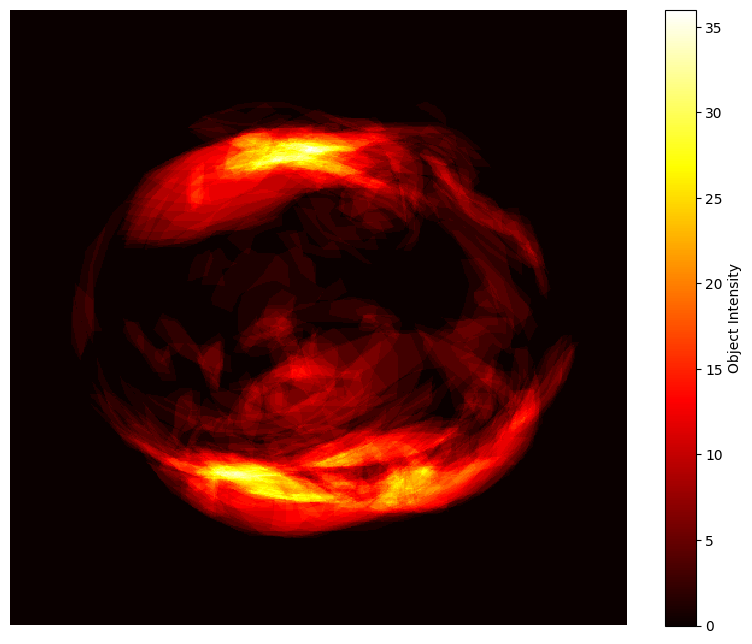
\includegraphics[width=1.0\linewidth]{Images/Chapter2/whole_heatmap}
\caption{ پراکندگی مکانی خونریزی در مجموعه‌داده
\lr{PhysioNet}}
\label{fig:ch3-wholeheatmap}
\end{figure}


\begin{figure}[h!]
    \centering % Center the figure
    \begin{subfigure}{0.33\textwidth}
        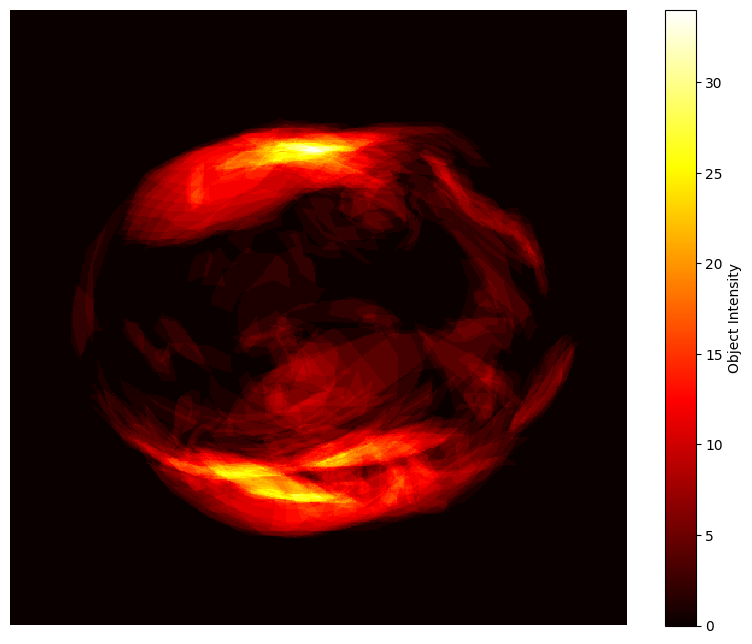
\includegraphics[width=\linewidth]{Images/chapter2/fold0_heatmap.png}
        \caption{\lr{Fold 0}}
        \label{fig:fold0}
    \end{subfigure}\hfil % Space between images
    \begin{subfigure}{0.33\textwidth}
        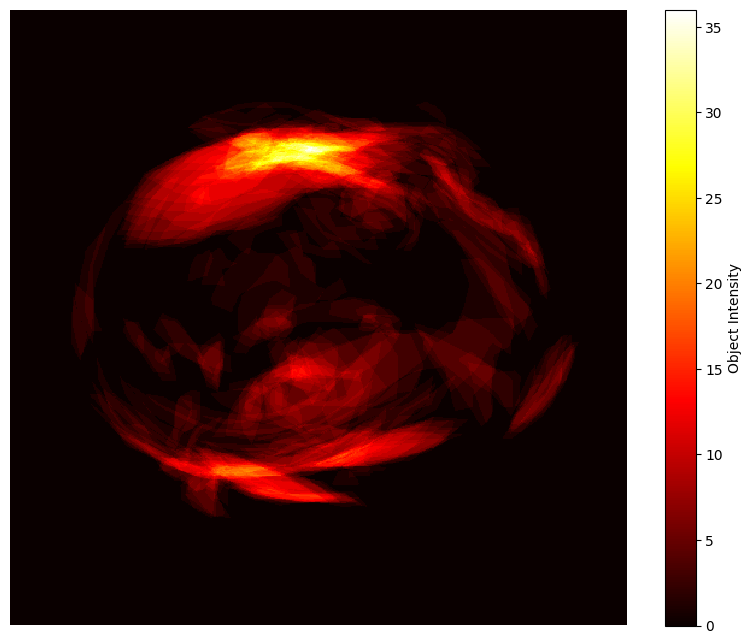
\includegraphics[width=\linewidth]{Images/chapter2/fold1_heatmap.png}
        \caption{\lr{Fold 1}}
        \label{fig:fold1}
    \end{subfigure}\hfil
    \begin{subfigure}{0.33\textwidth}
        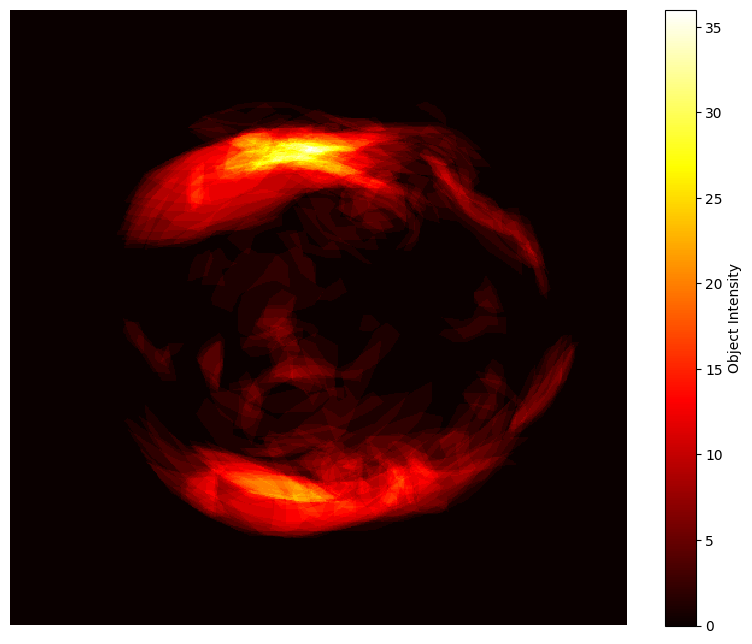
\includegraphics[width=\linewidth]{Images/chapter2/fold2_heatmap.png}
        \caption{\lr{Fold 2}}
        \label{fig:fold2}
    \end{subfigure}

    \vspace{1em} % Add vertical space between rows

    \begin{subfigure}{0.33\textwidth}
        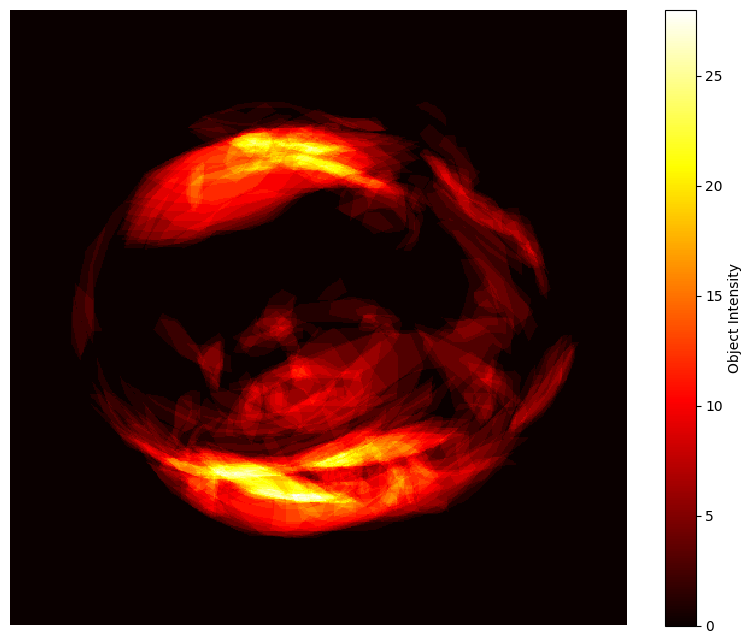
\includegraphics[width=\linewidth]{Images/chapter2/fold3_heatmap.png}
        \caption{\lr{Fold 3}}
        \label{fig:fold3}
    \end{subfigure}\hfil
    \begin{subfigure}{0.33\textwidth}
        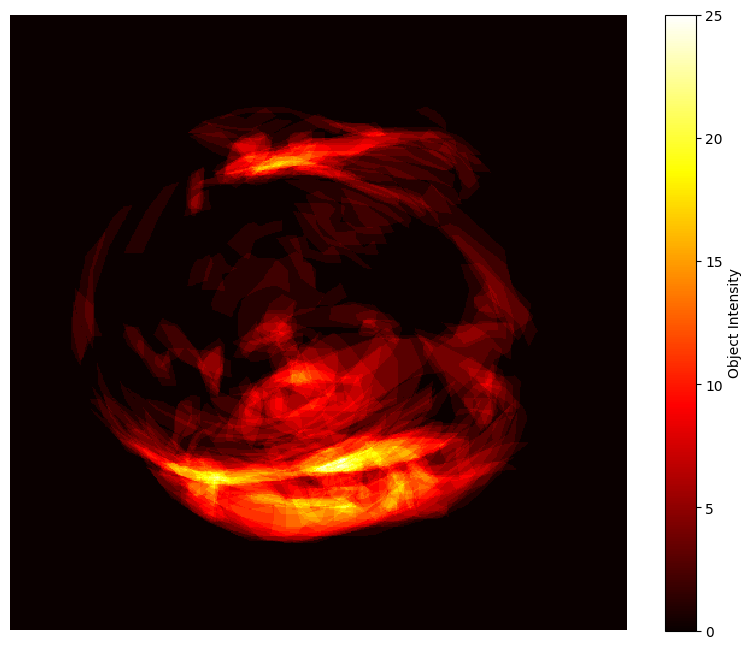
\includegraphics[width=\linewidth]{Images/chapter2/fold4_heatmap.png}
        \caption{\lr{Fold 4}}
        \label{fig:fold4}
    \end{subfigure}\hfil
    \begin{subfigure}{0.33\textwidth}
        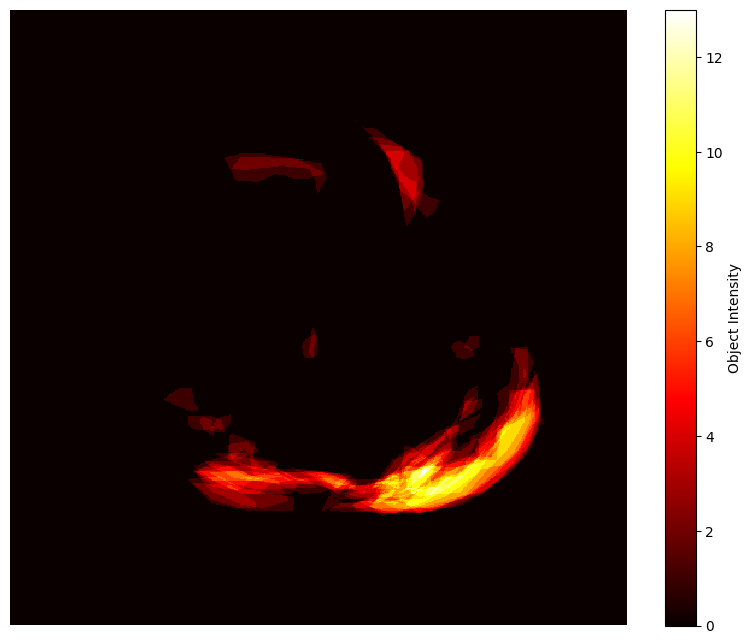
\includegraphics[width=\linewidth]{Images/chapter2/test_heatmap.png}
        \caption{مجموعه ارزیابی}
        \label{fig:test}
    \end{subfigure}

    \caption{پراکندگی مکانی خونریزی در زیرمجموعه‌های متفاوت از مجموعه‌داده}
    \label{fig:heatmaps}
\end{figure}


\section{پیش‌پردازش\protect\LTRfootnote{Pre-process}}

در تصاویر پرتونگاری سی‌تی‌اسکن، از اشعه ایکس
\LTRfootnote{X-Ray}
 به‌منظور ثبت تصویر اندام درونی بدن استفاده می‌شود. در این روش، ‌یک کاتد
 \LTRfootnote{Cathode}
را برانگیخته می‌کنند تا الکترون‌های
 \LTRfootnote{Electron}
 پرانرژی را آزاد ‌کند. با آزادشدن الکترون‌ها، انرژی به‌صورت اشعه ایکس آزاد می‌شود و اشعه ایکس از بافت‌ها عبور کرده و به آشکارساز در سمت دیگر برخورد می‌کند. هرچه بافت متراکم‌تر باشد، اشعه ایکس بیشتری را جذب می‌کند؛ مثلا بافت استخوانی به علت تراکم بالا،‌ اشعه ایکس بیشتری جذب می‌کند و در نتیجه آن اشعه کمتری به آشکارساز می‌رسد که موجب سفیدشدن آن قسمت از تصویر خواهد شد؛ اما این مسئله درمورد هوا برعکس است
 \cite{kaggleCTScansDICOM}.
در مقایسه با تصویر اشعه ایکس ساده، سی‌تی‌اسکن دارای تفکیک‌پذیری بیشتر است و هیچ هم‌پوشانی در ساختارها وجود ندارد.
دستگاه‌های سی‌تی‌اسکن که از کالیبراسیون
\LTRfootnote{Calibration}
 درستی برخوردار باشند، تصاویر خود را طبق یکای 
 \lr{Hounsfield}
ثبت می‌کنند. این یکا به پرتونگارها و محققین اجازه می‌دهد تا بتوانند با آستانه‌گذاری مناسب، جزئیات بافت هدف خود را در تصویر رؤیت‌پذیرتر کنند. تصاویر سی‌تی‌اسکن به‌صورت معمول بر اساس یکای
\lr{Hounsfield}
 مقادیر پیکسلی بین $-1024$ تا $3000$ را دارا هستند.

\autoref{fig:ch2-hu}
نشان‌دهنده مقدار پیکسلی است که هر بافت در تصویر سی‌تی‌اسکن از خود نشان می‌دهد. پروتونگارها،‌ پزشک‌ها و محققین برای اینکه بتوانند یک بیماری خاص را مورد بررسی قرار بدهند، برش‌های تصاویر را در بازه‌های خاصی از یکای
\lr{Hounsfield}
مورد بررسی قرار می‌دهند که به این نوع از پیش‌پردازش تصاویر سی‌تی‌اسکن،‌پنجره‌گذاری
\LTRfootnote{Windowing}
می‌گویند. 
\begin{figure}[H]
\centering
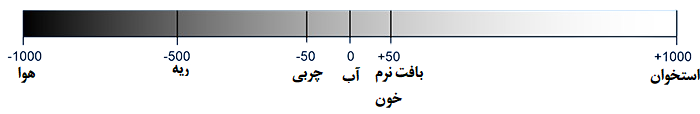
\includegraphics[width=1.0\linewidth]{Images/Chapter2/HU}
\caption{اثر بافت‌های متفاوت در یکای
 \lr{Hounsfield}
 \cite{kaggleCTScansDICOM}}
\label{fig:ch2-hu}
\end{figure}

در روش پنجره‌گذاری، دو مقدار مرکز پنجره
\lr{(WC)}
و پهنای پنجره
\lr{(WW)}
بازه هدف را در تصویر مشخص می‌کند و به‌موجب آن هر پیکسل که مقدار آن از حداقل بازه کمتر باشد، مقدارش برابر با حداقل بازه می‌شود و هر پیکسل که مقدارش از حداکثر بازه بیشتر باشد، مقدارش برابر حداکثر بازه می‌شود. ‎
\autoref{code:ch2-windowing}
روش اعمال پنجره‌گذاری روی تصاویر را نمایش می‌دهد که در آن 
\lr{Normalize}
به‌منظور انتقال مقادیر تصویر بعد از پنجره‌گذاری بین 0 و 1 است و 
\lr{Threshold}
تابعی است که در اثر آن مقادیر کمتر از حداقل بازه هدف به مقدار حداقل تغییر پیدا می‌کنند و مقادیری بیشتر از حداکثر بازه به مقدار حداکثر تبدیل می‌شوند.   
\begin{latin}
\begin{equation}
\text{Processed Image} = \text{Normalize}(\text{Threshold}(\text{Image}, WC-\frac{WW}{2},WC+\frac{WW}{2})) 
\end{equation}
\label{code:ch2-windowing}
\end{latin}

پرتونگار‌ها مقادیر مشخصی را برای شناسایی انواع مختلف اندام در تصاویر سی‌تی‌اسکن تعیین کرده‌اند به‌عنوان مثال، در مجموعه‌داده
\lr{‌PhysioNet}،
پردازش تصویر اصلی به‌ازای مرکز پنجره 40 و پهنای پنجره 120، پنجره مغز استخراج می‌شود و به‌ازای مرکز پنجره 700 و پهنای پنجره 3200،‌ پنجره استخوان استخراج می‌شود.
\autoref{fig:ch2-windowed-ct-sample}
اثر پنجره‌گذاری را بر یک نمونه برش سی‌تی‌اسکن نشان می‌دهد. همانطور که از این
\autoref{fig:ch2-before-processing}
 مشخص است، تصویر قبل از پیش‌پردازش جزئیات خاصی را به ما نشان نمی‌دهد و اگر این تصویر را بدون نرمال کردن برای آموزش شبکه‌ عصبی استفاده کنیم، باعث می‌شود که لایه‌های ابتدایی شبکه مقادیر خیلی بزرگی را ایجاد کنند و در نتیجه عملکرد مدل کاهش پیدا بکند و اگر این تصویر را نرمال کنیم، به علت بازه بسیار زیاد یکای 
\lr{Hounsfield}
تفکیک‌پذیری مقادیر تصویر به‌شدت کاهش پیدا می‌کند. در ادامه
\autoref{fig:ch2-brain-window}, \autoref{fig:ch2-bone-window} و \autoref{fig:ch2-subdural-window}
اثر سه پنجره مرسوم مغز، استخوان و سابدورال را مشاهده می‌کنیم که هرکدام تفکیک‌پذیری بافت هدف خود را افزایش داده‌اند و در پنجره مغز و سابدورال، محل خونریزی به‌وضوح مشخص است.
\autoref{fig:ch2-selected-window}
 پنجره انتخابی را نشان می‌دهد که بر اساس محدوده موجود در  
\autoref{fig:ch2-pixel-hist-ich-vs-healthy}
انتخاب شده ‌است و در نتیجه آن، محل خونریزی بروز بیشتری پیدا کرده است. در ادامه این پژوهش،‌ پنجره مغز به‌عنوان پنجره اصلی آموزش و ارزیابی مدل‌ها در نظر گرفته شده است.

از دیگر روش‌های پیش‌پردازشی که در این پروژه استفاده شده است، افزایش مصنوعی داده است که به جهت بهبود عملکرد مدل در فرایند آموزش انجام شده است. تبدیل‌های افزایش مصنوعی داده‌ای که در این پژوهش استفاده شده است شامل چرخش، برش تصادفی،‌ تبدیل آیینه حول محور افقی و‌ بزرگ‌نمایی تصادفی است. به علت اینکه سر تمامی بیماران در مجموعه‌داده 
\lr{PhysioNet}
جهت یکسانی دارد، استفاده از تبدیل آیینه حول محور عمودی باعث ایجاد تصاویری می‌شود که معادل آنها در مجموعه‌داده وجود ندارد
\cite{hssayeni2020intracranial}.



\begin{figure}[h!]
    \centering % <-- added
    \begin{subfigure}{0.33\textwidth}
      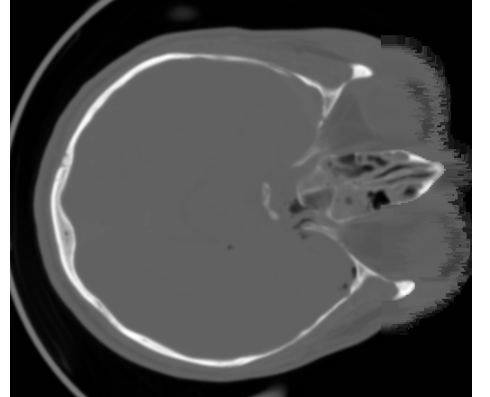
\includegraphics[width=\linewidth]{Images/chapter2/before_processing_no_caption.png}
      \caption{قبل از پردازش}
      \label{fig:ch2-before-processing}
    \end{subfigure}\hfil % <-- 
    \begin{subfigure}{0.33\textwidth}
      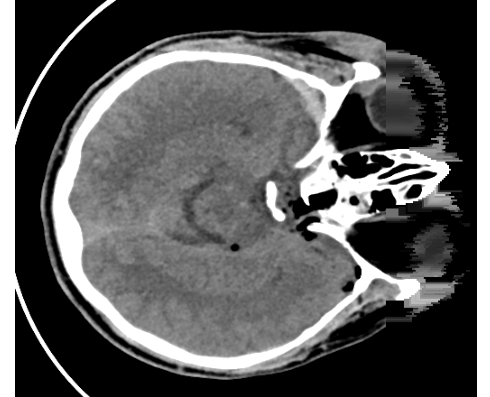
\includegraphics[width=\linewidth]{Images/chapter2/brain_window_no_caption.png}
      \caption{پنجره مغز}
      \label{fig:ch2-brain-window}
    \end{subfigure}\hfil % <-- 
    \begin{subfigure}{0.33\textwidth}
      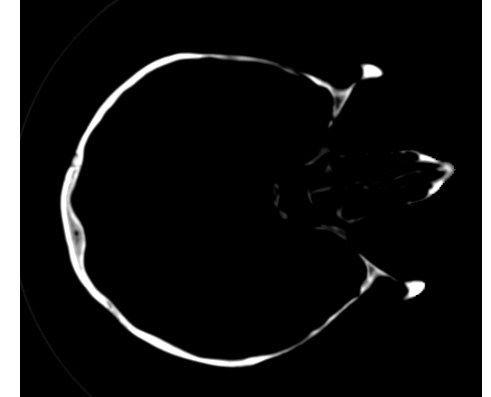
\includegraphics[width=\linewidth]{Images/chapter2/bone_window_no_caption.png}
      \caption{پنجره استخوان}
      \label{fig:ch2-bone-window}
    \end{subfigure}\hfil % <-- 
    \begin{subfigure}{0.33\textwidth}
      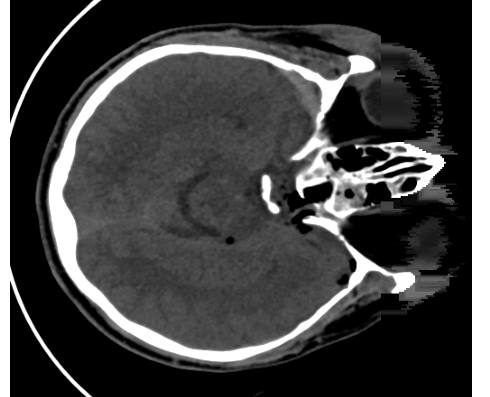
\includegraphics[width=\linewidth]{Images/chapter2/subdural_window_no_caption.png}
      \caption{پنجره ساب‌دورال}
      \label{fig:ch2-subdural-window}
    \end{subfigure}\hfil % <-- 
    \begin{subfigure}{0.33\textwidth}
      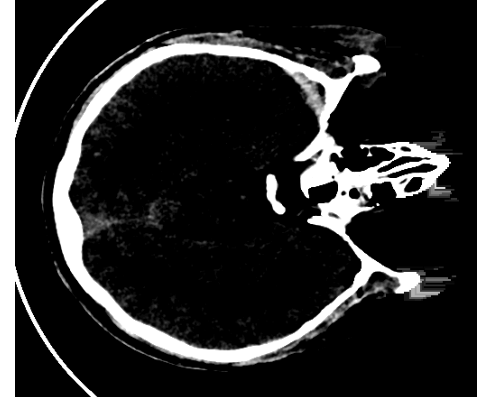
\includegraphics[width=\linewidth]{Images/chapter2/selected_window_no_caption.png}
      \caption{پنجره انتخابی}
      \label{fig:ch2-selected-window}
    \end{subfigure}\hfil % <-- 
    \begin{subfigure}{0.33\textwidth}
      
\includegraphics[width=\linewidth]{Images/chapter2/bleed_location_no_caption.png}
      \caption{محل خونریزی}
      \label{fig:ch2-bleed-location}
    \end{subfigure}
\caption{تأثیر پنجره‌گذاری در نمایش خونریزی در یک برش از سی‌تی‌اسکن}
\label{fig:ch2-windowed-ct-sample}
\end{figure}

\section{روش پردازش تصاویر}
شبکه‌های عصبی عمیق به‌عنوان یکی از روش‌های محبوب در حوزه‌ی یادگیری ماشین شناخته می‌شوند. این شبکه‌ها از ساختارهایی شبیه به مغز انسان تشکیل شده‌اند که شامل تعدادی نورون \LTRfootnote{Neuron} مصنوعی هستند و قادرند با استفاده از داده‌های ورودی، الگوها و روابط پیچیده را بیاموزند. یادگیری عمیق، شاخه‌ای از شبکه‌های عصبی است که با افزایش تعداد لایه‌های مخفی در شبکه، امکان پردازش و تحلیل داده‌های بسیار پیچیده و بزرگ را فراهم می‌کند.
در این پژوهش، روش اصلی مورداستفاده برای پردازش کامپیوتری تصاویر، یادگیری عمیق است.
\subsection{یادگیری عمیق و اصول اولیه}
یادگیری عمیق یکی از شاخه‌های مهم یادگیری ماشین است که به دلیل توانایی‌های خود در پردازش، تحلیل و الگویابی در داده‌های پیچیده، به‌ویژه در حوزه‌ی پزشکی، به به‌صورت گسترده‌ای مورداستفاده قرار گرفته است. در این بخش، به بررسی اصول پایه‌ای یادگیری عمیق در پردازش تصویر پرداخته شده است.

\subsubsection{ساختار نورون}
شبکه‌های عصبی مصنوعی از تعدادی واحد پردازشی به نام نورون تشکیل شده‌اند. هر نورون چندین ورودی \(x_1, x_2, \ldots, x_n\) دریافت می‌کند که هر یک با وزن‌های \(w_1, w_2, \ldots, w_n\) متناظر ضرب می‌شوند. سپس، مجموع وزن‌دار ورودی‌ها به اضافه‌ی یک بایاس \(b\) مطابق با \autoref{eq:sum_weights} محاسبه شده و از طریق یک تابع فعال‌سازی \(\phi\) به خروجی تبدیل می‌شود که رابطه آن در \autoref{eq:activation} مشخص شده است.

\begin{latin}
\begin{equation}
\label{eq:sum_weights}
z = \sum_{i=1}^{n} w_i x_i + b
\end{equation}
\end{latin}

\begin{latin}
\begin{equation}
\label{eq:activation}
a = \phi(z)
\end{equation}
\end{latin}

توابع فعال‌سازی به‌منظور ایجاد خاصیت غیرخطی در نورون‌ها استفاده ‌می‌شوند تا با استفاده از شبکه عصبی عمیق،‌ بتوانیم توابع غیرخطی را تخمین بزنیم. دو تابع فعال‌سازی رایج عبارت‌اند از
 \lr{ReLU}\LTRfootnote{Rectified Linear Unit} و
 \lr{Sigmoid}\LTRfootnote{Sigmoid}.
  رابطه تابع
   \lr{ReLU}
    در
     \autoref{eq:relu}
      مشخص شده است و رابطه تابع 
      \lr{Sigmoid}، 
      در
      \autoref{eq:sigmoid}
      مشخص شده است.

\begin{latin}
\begin{equation}
\label{eq:relu}
\phi(z) = \max(0, z)
\end{equation}
\end{latin}

\begin{latin}
\begin{equation}
\label{eq:sigmoid}
\phi(z) = \frac{1}{1 + e^{-z}}
\end{equation}
\end{latin}


\subsubsection{لایه‌های پنهان}
شبکه‌های عصبی عمیق از چندین لایه‌ی پنهان تشکیل شده‌اند که هر کدام از تعداد زیادی نورون مشابه نورون‌های توصیف‌شده در بخش قبلی تشکیل شده‌اند. خروجی هر نورون در یک‌لایه به‌عنوان ورودی برای نورون‌های لایه‌ی بعدی استفاده می‌شود. این ساختار چندلایه به شبکه امکان می‌دهد تا ویژگی‌های پیچیده و  رفتار غیرخطی را از داده‌های ورودی استخراج کند.
\autoref{fig:ch2-neuron}
نمایش نحوه مدل‌سازی یک نورون را با استفاده از 
\autoref{eq:sum_weights} و \autoref{eq:activation}
نشان می‌دهد و در ادامه نحوه عملکرد لایه‌های پنهان در شبیه‌سازی ارتباط بین نورون‌ها را نشان می‌دهد. 
\begin{figure}[h]
\centering
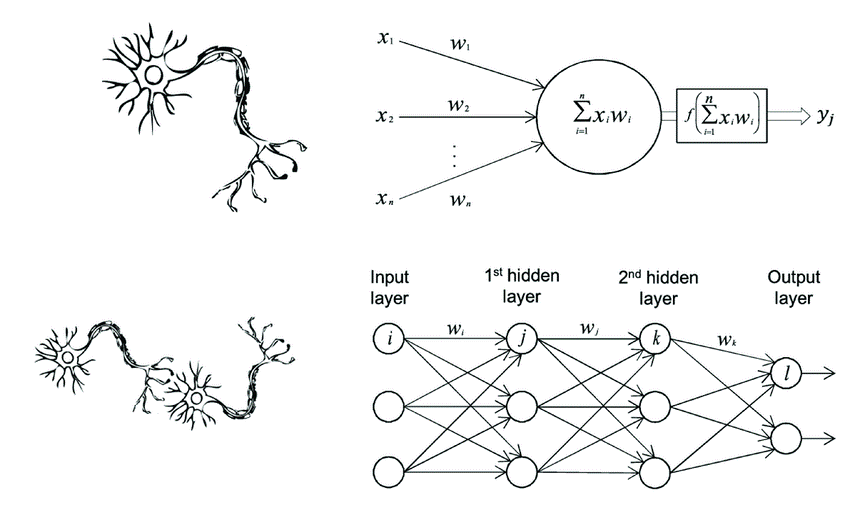
\includegraphics[width=1.0\linewidth]{Images/Chapter2/neuron}
\caption{مدلسازی یک نورون عصبی توسط رابطه ریاضی و ارتباط بین نورون‌ها با استفاده از لایه‌های پنهان
\cite{brainmentorsIntroductionDeep}}
\label{fig:ch2-neuron}
\end{figure}


\subsubsection{تابع خطا و پس‌انتشار
\protect\LTRfootnote{backpropagation}}
تابع خطا
 \LTRfootnote{Loss Function}
  نقش کلیدی در آموزش شبکه‌های عصبی دارد. این تابع تفاوت بین خروجی پیش‌بینی‌شده
  \lr{ \(y_{\text{pred}}\)}
   و خروجی واقعی
    \lr{\(y_{\text{true}}\)}
     را محاسبه می‌کند. یکی از رایج‌ترین توابع خطا، خطای 
  \lr{Binary Cross Entropy(BCE)}
   است که طبق 
   \autoref{eq:bce_loss}
   برای مسائل دسته‌بندی دوتایی استفاده می‌شود.

\begin{latin}
\begin{equation}
\label{eq:bce_loss}
L(\mathbf{y}_{\text{true}}, \mathbf{y}_{\text{pred}}) = -\frac{1}{m} \sum_{i=1}^{m} \left[ y_{\text{true}}^{(i)} \log(y_{\text{pred}}^{(i)}) + (1 - y_{\text{true}}^{(i)}) \log(1 - y_{\text{pred}}^{(i)}) \right]
\end{equation}
\end{latin}


هدف از آموزش شبکه، کمینه‌سازی این تابع خطا است که با استفاده از الگوریتم پس‌انتشار انجام می‌شود. در این روش، گرادیان
\LTRfootnote{Gradient}
 تابع خطا نسبت به هر وزن \(w_i\) طبق \autoref{eq:gradient} و قانون مشتقات زنجیره‌ای، محاسبه شده و سپس وزن‌ها با استفاده از روش گرادیان کاهشی مطابق \autoref{eq:weight_update} به‌روزرسانی می‌شوند.

\begin{latin}
\begin{equation}
\label{eq:gradient}
\frac{\partial L}{\partial w_i}
\end{equation}
\end{latin}

\begin{latin}
\begin{equation}
\label{eq:weight_update}
w_{i+1} \leftarrow w_i - \eta \frac{\partial L}{\partial w_i}
\end{equation}
\end{latin}

\subsubsection{لایه‌های پرسپترون
\protect\LTRfootnote{Perceptron}
 چندلایه}
لایه‌های پرسپترون چندلایه
 \lr{(MLP)} 
 یکی از ساده‌ترین و پایه‌ای‌ترین ساختارها در شبکه‌های عصبی هستند. این لایه‌ها از تعدادی نورون تشکیل شده‌اند که به‌صورت کامل به یکدیگر متصل هستند؛ به بیان دیگر هر نورون در یک لایه به‌تمامی نورون‌های لایه‌ی قبلی متصل می‌شود و اطلاعات را به لایه‌ی بعدی منتقل می‌کند. خروجی هر لایه \(a^{[l]}\) از ترکیب خطی ورودی‌ها و اعمال تابع فعال‌سازی طبق \autoref{eq:mlp_output} به دست می‌آید:

\begin{latin}
\begin{equation}
\label{eq:mlp_output}
a^{[l]} = \phi(W^{[l]} a^{[l-1]} + b^{[l]})
\end{equation}
\end{latin}

\subsubsection{شبکه عصبی پیچشی
\protect\LTRfootnote{Convolutional Neural Network}}
برای بهبود عملکرد شبکه‌های عصبی در پردازش تصاویر، از لایه‌های شبکه عصبی پیچشی
\lr{(CNN)} 
استفاده می‌شود. در این لایه‌ها، عملیات کانولوشن به‌جای ضرب ماتریسی بین ورودی و وزن‌ها طبق \autoref{eq:convolution} انجام می‌شود. این عملیات برای هر ناحیه کوچک از تصویر با استفاده از یک فیلتر \(k\) صورت می‌گیرد.

\begin{latin}
\begin{equation}
\label{eq:convolution}
z_{i,j} = (X * k)_{i,j} = \sum_{m}\sum_{n} X_{i+m,j+n} \cdot k_{m,n}
\end{equation}
\end{latin}

خروجی این عملیات، نقشه ویژگی
\lr{Feature Map}
 است که به لایه بعدی منتقل می‌شود. با عبور یک تصویر از لایه‌های یک شبکه عصبی پیچشی، بین پیکسل‌های مجاور هم در تصویر، یک رابطه برقرار می‌شود که درنتیجه آن، نقشه ویژگی استخراج شده برای هر پیکسل،‌ به وضعت پیکسل‌های اطرافش بستگی دارد و هرچه از پیکسل مبدأ دور شویم، اثر آن در نقشه ویژگی کاهش پیدا می‌کند.
 
 

\subsubsection{بهینه‌سازها و الگوریتم 
\lr{Adam}
}

بهینه‌سازی یکی از مهم‌ترین اجزا در آموزش شبکه‌های عصبی هستند که هدف آنها به‌روزرسانی وزن‌ها به‌گونه‌ای است که تابع خطا به حداقل مقدار خود برسد. برای این منظور، از الگوریتم‌هایی استفاده می‌شود که بهینه‌ساز نامیده می‌شوند. 
یکی از رایج‌ترین بهینه‌سازها، الگوریتم گرادیان کاهشی است که در آن وزن‌ها در جهت منفی گرادیان تابع خطا به‌روزرسانی می‌شوند، رابطه گرادیان کاهشی در \autoref{eq:weight_update} نشان داده شده است. 
 یکی دیگر از بهینه‌سازهای پیشرفته و کارآمد، بهینه‌ساز 
\lr{Adam}
 است. این بهینه‌ساز از ترکیب دو روش
\lr{Momentum}
 و
\lr{RMSProp}
 بهره می‌برد 
 \cite{towardsdatascienceUnderstandingDeep,mediumMomentumRMSpropAdam}.
  به‌روزرسانی وزن‌ها در \lr{Adam} با استفاده از روابط در 
  \autoref{eq:adam}
  انجام می‌شود.

\begin{latin}
\begin{equation}
\label{eq:adam}
\begin{aligned}
m_t &= \beta_1 m_{t-1} + (1 - \beta_1) \nabla L(\theta_t)\\
v_t &= \beta_2 v_{t-1} + (1 - \beta_2) (\nabla L(\theta_t))^2\\
\theta_{t+1} &= \theta_t - \eta \frac{\hat{m}_t}{\sqrt{\hat{v}_t} + \epsilon}
\end{aligned}
\end{equation}
\end{latin}


در این معادلات، \(m_t\) و \(v_t\) به ترتیب تخمین میانگین حرکت‌دار گرادیان و میانگین حرکت‌دار مربعات گرادیان در زمان \(t\) هستند، و \(\beta_1\) و \(\beta_2\) ضرایب مربوط به این میانگین‌ها هستند. \(\eta\) نرخ یادگیری و \(\epsilon\) یک مقدار بسیار کوچک برای جلوگیری از تقسیم بر صفر است. الگوریتم
\lr{Adam} 
به دلیل عملکرد مناسب خود در آموزش شبکه‌های عصبی عمیق، به یکی از بهینه‌سازهای پرکاربرد در این زمینه تبدیل شده است.


\section{مدل‌های طبقه‌بندی در شبکه عصبی عمیق}

\subsection{\lr{ResNet}}
\label{ResNet subsection}
شبکه‌های عصبی عمیق به یک ابزار قدرتمند در انجام وظایف مختلف یادگیری ماشین تبدیل شده‌اند. بااین‌حال، با افزایش عمق این شبکه‌ها، مشکلاتی همچون ناپدیدشدن مشتق
\LTRfootnote{Vanishing Gradient}
یا انفجار مشتق 
\LTRfootnote{Exploding Gradient}
 و دشوارشدن آموزش به ‌وجود می‌آید. برای حل این مشکلات،
  \lr{He}\cite{he2016deep}
   و همکارانش معماری شبکه‌های 
   \lr{ResNet}
   را پیشنهاد کردند که امکان آموزش شبکه‌های بسیار عمیق‌تر را با معرفی اتصالات 
   \lr{Residual}
   فراهم می‌کند.
ایده اصلی پشت 
\lr{ResNet}
 معرفی یک اتصال  میان‌بر
 \LTRfootnote{Skip Connection}
 است که یک یا چند لایه از شبکه را دور می‌زند. این اتصال  میان‌بر به شبکه امکان می‌دهد تا از طریق آن، مشتق خطا به لایه‌های ابتدایی برسد تا فرایند آموزش برای لایه‌هایی که از خروجی دور هستند، با مشکل مواجه نشود.همانطور که در 
 \autoref{fig:ch-2resnet_block}
 نمایش‌داده‌‌شده است، در شبکه‌های 
 \lr{ResNet}
 به‌جای یادگیری یک نگاشت مستقیم، مثلاً $H(x)$، شبکه نگاشت $F(x) = H(x) - x$ را یاد می‌گیرد که بهینه‌سازی آن ساده‌تر است؛ بنابراین، خروجی نهایی بلوک
 \LTRfootnote{Block}
  $H(x) = F(x) + x$ خواهد بود که در نتیجه آن، مشتق
 تابع خطای $L$ به‌ازای ورودی $x$ در 
 \autoref{eq:ch2-resnet-deriviation}
 نمایش‌‌داده‌شده است.
 
\begin{latin}
\begin{equation}
\label{eq:ch2-resnet-deriviation}
\begin{aligned}
 \frac{\partial L}{\partial x} = \frac{\partial L}{\partial H(x)} \cdot \frac{\partial H(x)}{\partial x} = \frac{\partial L}{\partial H(x)} \cdot \left(1 + \frac{\partial F(x)}{\partial x}\right)
\end{aligned}
\end{equation}
\end{latin}

 
 این فرمول نشان می‌دهد که مشتق می‌تواند به‌راحتی از طریق مسیر  میان‌بر عبور کند که به حل مشکل ناپدیدشدن یا انفجار گرادیان کمک می‌کند.
 
\begin{figure}[h]
    \centering
    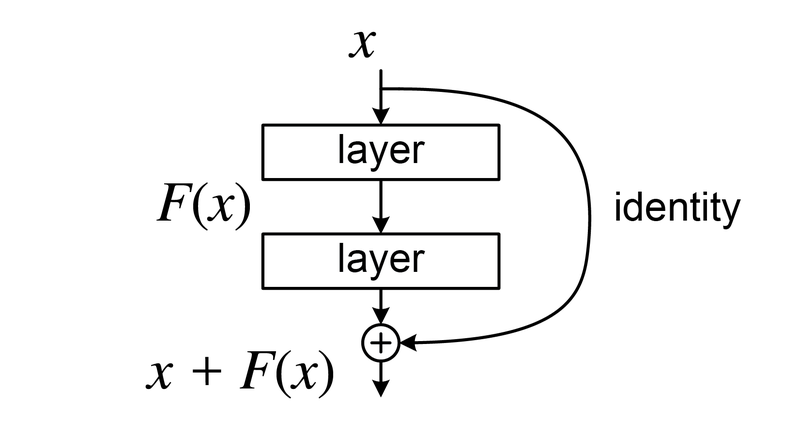
\includegraphics[width=0.6\textwidth]{Images/Chapter2/ResBlock.png}
    \caption{یک بلوک از معماری 
    \lr{ResNet} 
    که اتصال  میان‌بر همانی را نشان می‌دهد
    \cite{wikipediaResidualNeural}.}
    \label{fig:ch-2resnet_block}
\end{figure}
شبکه عصبی پیچشی 
\lr{ResNet}
 در وظیفه طبقه‌بندی تصویر عملکرد مناسبی از خود نشان داده است. این شبکه با معرفی اتصال  میان‌بر و  فراهم‌کردن امکان آموزش شبکه‌های بسیار عمیق، باعث بهبود عملکرد مدل‌های شبکه عصبی عمیق شده‌ است.


\subsection{\lr{ResNeXt}}

\lr{ResNeXt}
توسط 
\lr{Xie}\cite{xie2017aggregated}
و همکاران معرفی شده است که 
یک معماری شبکه عصبی پیچشی عمیق است که بر اساس ساختار 
\lr{ResNet}
ساخته شده و با معرفی یک فراپارامتر
\LTRfootnote{Hyper-parameter}
 جدید به نام کاردینالیتی
\LTRfootnote{Cardinality} 
  سعی در بهبود مدل 
  \lr{ResNet}
  داشته است.
 این مدل به‌منظور بهبود عملکرد شبکه‌های عصبی عمیق،  مسیرهای موازی متعدد را در ساختار شبکه ایجاد می‌کند که این روش مشابه مدل ساختار
  \lr{Inception} 
است؛ اما با تفاوت‌های کلیدی در سادگی طراحی اجزای شبکه.

همانطور که در 
\autoref{fig:ch2-resnext1}, \autoref{fig:ch2-resnext2}
مشخص شده است، مسیرهای موازی در ساختار شبکه ایجاد شده است که این مسیرها به مقدار کاردینالیتی بستگی دارد.
کاردینالیتی به تعداد مسیرهای موازی درون هر بلوک شبکه اشاره دارد. برخلاف افزایش عمق یا عرض که به افزایش تعداد لایه‌ها یا پیچیدگی هر لایه منجر می‌شود، افزایش کاردینالیتی اجازه می‌دهد که چندین مسیر پردازشی به‌صورت موازی عمل کنند و در نهایت خروجی‌های آن‌ها با یکدیگر ادغام شوند که از بار پردازشی شبکه کم می‌کند.
\autoref{fig:ch2-resnext3}
ساده‌سازی بلوک 
\lr{ResNeXt}
برای بهینه‌سازی و ساده‌سازی محاسبات را نشان می‌دهد که از لایه‌های پیچشی گروهی استفاده می‌کند. در این روش، کانال‌های 
\LTRfootnote{Channel}
ورودی به گروه‌های مختلف تقسیم می‌شوند و کانولوشن‌ها به‌صورت مستقل در هر گروه انجام می‌گیرند.
افزایش کاردینالیتی در \lr{ResNeXt} نه‌تنها باعث بهبود دقت مدل می‌شود، بلکه امکان استفاده از مسیرهای پردازشی متعدد به‌صورت موازی، بدون افزایش چشمگیر در پیچیدگی محاسباتی، را فراهم می‌کند. این ویژگی به \lr{ResNeXt} اجازه می‌دهد که در وظایف پیچیده، مانند طبقه‌بندی تصاویر با دقت بیشتری عمل کند. علاوه بر این، استفاده از لایه‌های پیچشی گروهی به کاهش هزینه محاسباتی کمک کرده و درعین‌حال، قدرت الگوهای پیچیده را حفظ می‌کند.

\begin{figure}[h!]
    \centering % <-- added
    \begin{subfigure}{0.33\textwidth}
        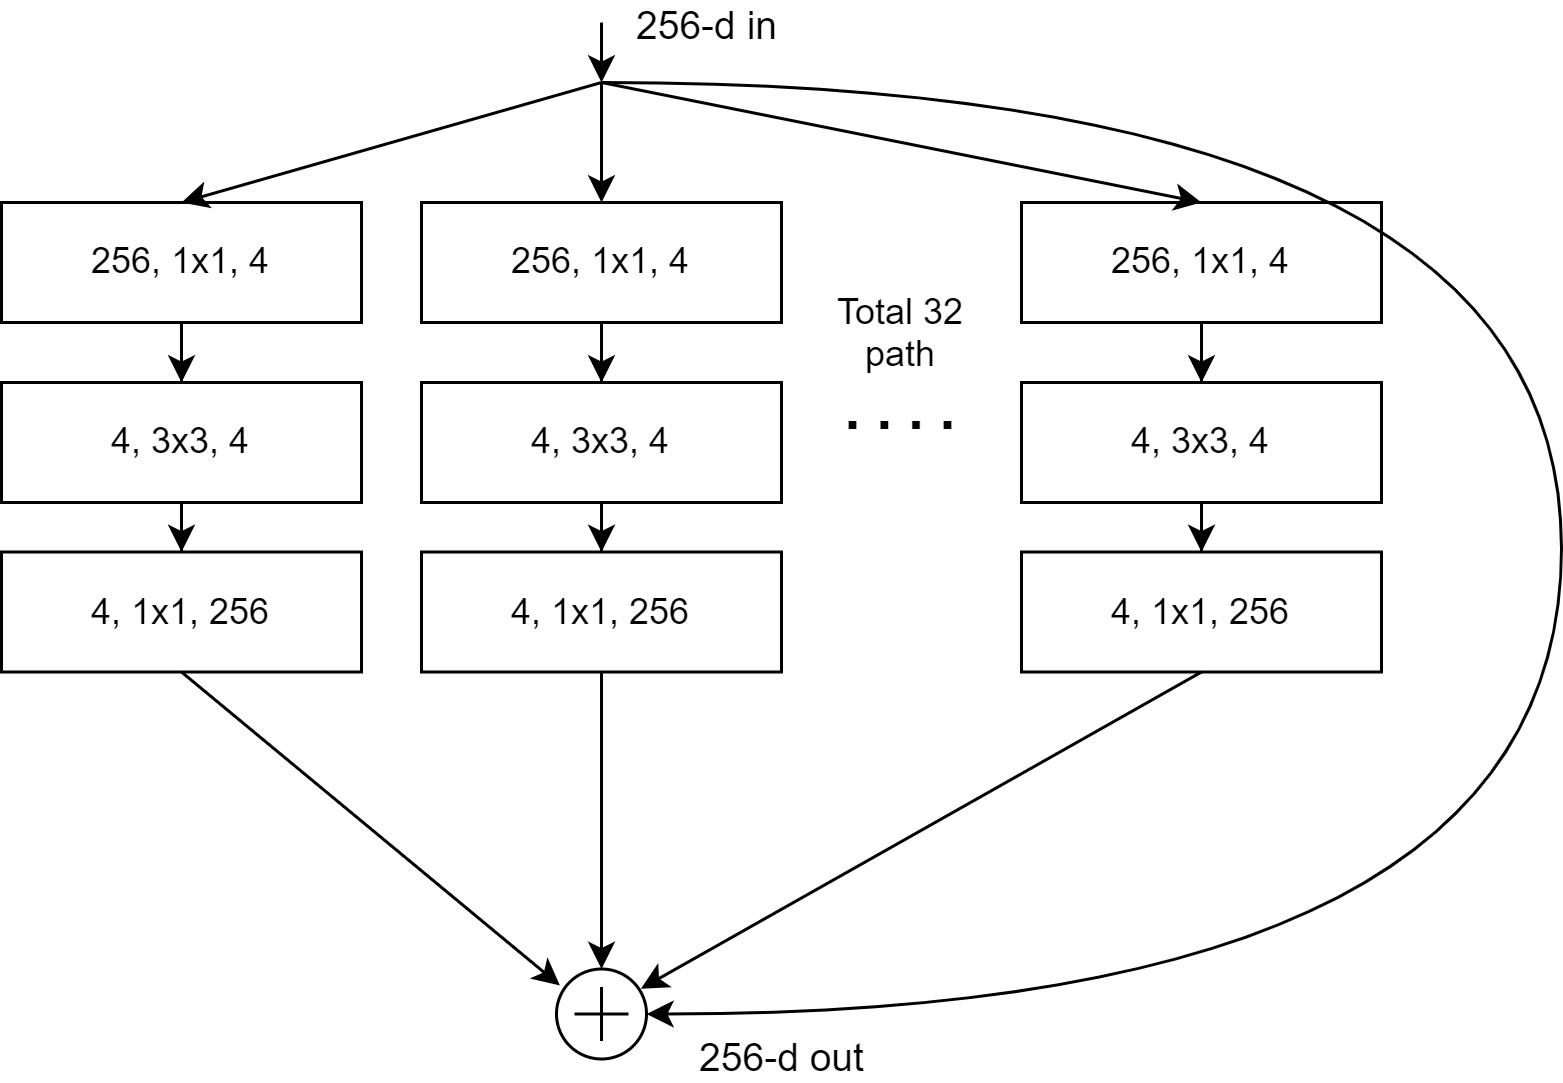
\includegraphics[width=\linewidth]{Images/Chapter2/resnext1.png}
        \caption{}
        \label{fig:ch2-resnext1}
    \end{subfigure}\hfil % <-- 
    \begin{subfigure}{0.33\textwidth}
        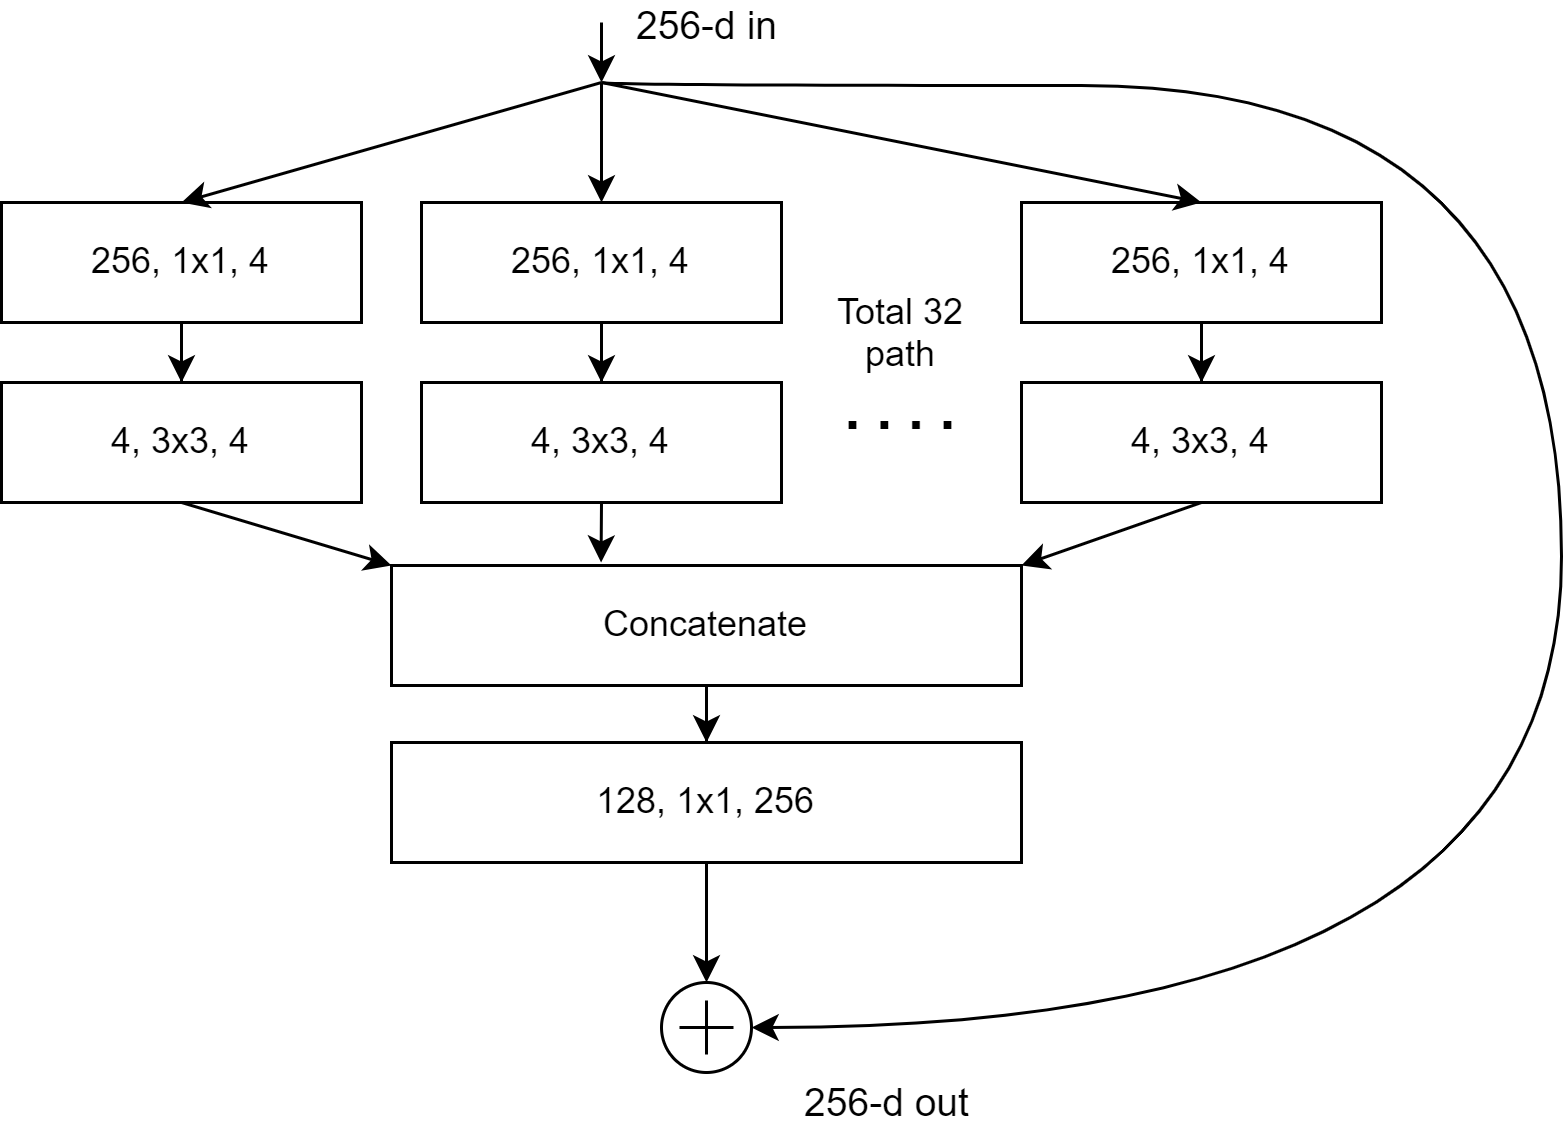
\includegraphics[width=\linewidth]{Images/Chapter2/resnext2.png}
        \caption{}
        \label{fig:ch2-resnext2}
    \end{subfigure}\hfil % <-- added
    \begin{subfigure}{0.33\textwidth}
        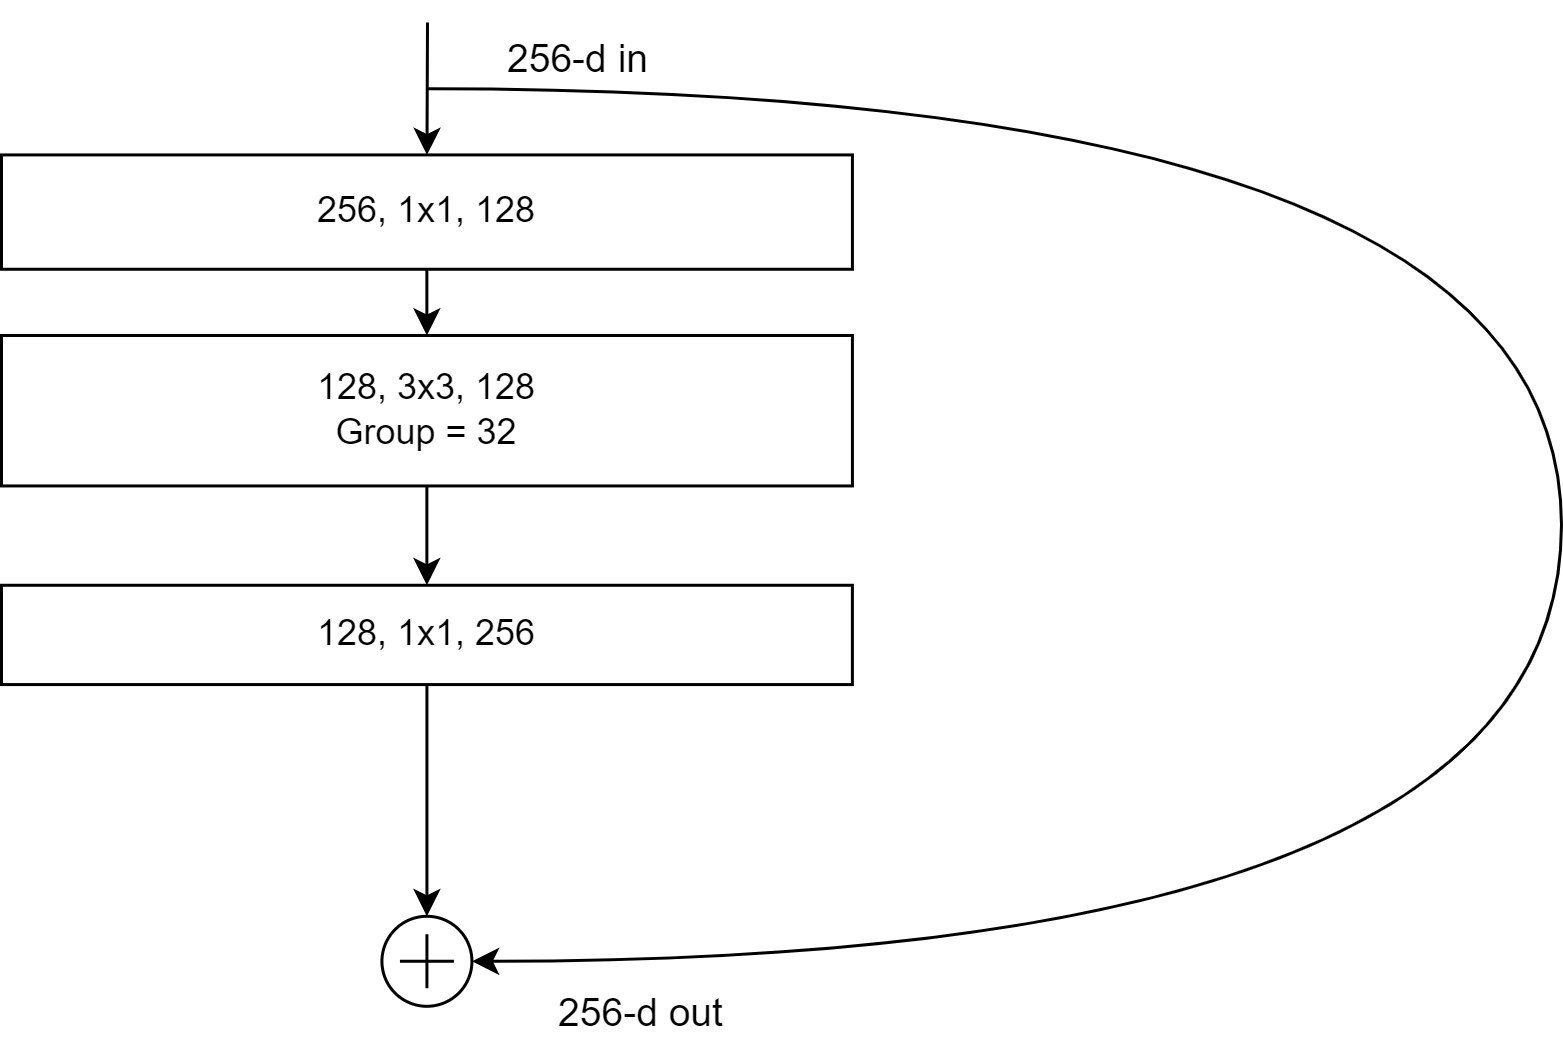
\includegraphics[width=\linewidth]{Images/Chapter2/resnext3.png}
        \caption{}
        \label{fig:ch2-resnext3}
    \end{subfigure}
    \caption{ساختارهای مختلف در معماری 
    \lr{ResNeXt}
     که کانولوشن‌های گروهی، مسیرهای پردازشی موازی و روش ادغام را نشان می‌دهند
     \cite{xie2017aggregated}.}
    \label{fig:fig:ch2-resnext}
\end{figure}







\subsection{شبکه
\lr{Squeeze-and-Excitation}
\lr{(SENet)}}

\lr{Hu}\cite{hu2018squeeze}
و همکاران،‌ با معرفی بلوک
 \lr{Squeeze-and-Excitation}
 \lr{(SE)}
 ، دقت طبقه‌بندی در \lr{ImageNet} به میزان 2.5\% نسبت به سال گذشته بهبود یافت. این بلوک با وزن‌دهی به میان کانال‌های مختلف در هر لایه از شبکه عصبی پیچشی، عملکرد شبکه‌های عصبی را با هزینه محاسباتی بسیار کمی بهبود می‌بخشد.
ایده اصلی درمورد روش 
 \lr{Squeeze-and-Excitation}
  این است که در یک لایه معمولی در شبکه عصبی پیچشی، ارزش هر کانال در ورودی شبکه، با بقیه کانال‌ها یکسان است. بلوک \lr{SE} اما، رویکردی تطبیقی را معرفی می‌کند که در آن اهمیت هر کانال به به‌صورت جداگانه و بر اساس زمینه ارزیابی می‌شود و به آن وزنی خاص اختصاص داده می‌شود.

\autoref{fig:se_block}
نحوه عملکرد این مدل را نشان می‌دهد که در گام نخست از هر کانال نقشه ویژگی، میانگین گرفته می‌شود، سپس این میانگین از یک تابع خطی عبور داده می‌شود و در گام بعدی، تابع 
\lr{Sigmoid}
روی آن اعمال می‌شود تا وزن‌ها بین 0 تا 1 قرار بگیرند.
در انتها وزن‌های محاسبه شده در نقشه ویژگی ضرب می‌شود و خروجی لایه پیچشی 
 \lr{Squeeze-and-Excitation}
 شبکه عصبی پیچشی به دست می‌آید.
 \lr{ResNeXt}
 یکی از مدل‌های پایه‌ای است که با استفاده از روش بلوک
 \lr{SE}
 عملکردش ارتقا پیدا کرده است.
 
\begin{figure}[h!]
    \centering
    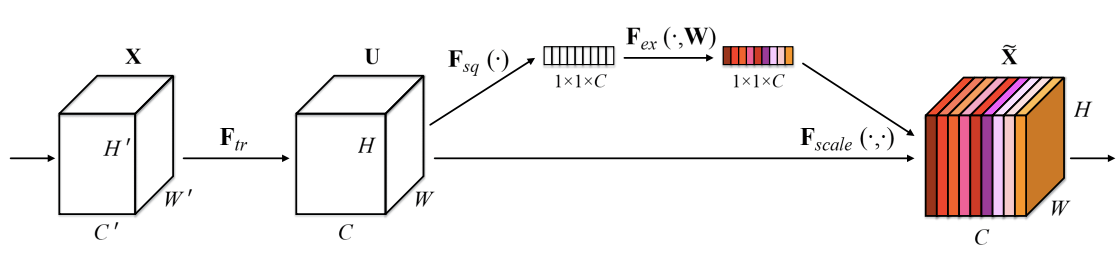
\includegraphics[width=1\textwidth]{Images/Chapter2/squeeze and excitation.png}
    \caption{بلوک \lr{Squeeze-and-Excitation} که نحوه عملکرد آن را در ارزیابی و وزن‌دهی کانال‌ها نشان می‌دهد \cite{hu2018squeeze}.}
    \label{fig:se_block}
\end{figure}




\subsection{\lr{DenseNet}}

\lr{DenseNet}
یک نوع شبکه‌ عصبی پیچشی است که به‌منظور بهبود عملکرد شبکه‌های عصبی پیچشی سنتی معرفی شده ‌است. یی این شبکه، کاهش محدودیت‌هایی است که معمولاً شبکه‌های پیچشی عمیق، با آن‌ها مواجه می‌شوند.
در شبکه‌های پیچشی سنتی، یکی از مشکلات اصلی زمانی رخ می‌دهد که مشتق، نمی‌تواند در فرایند پس‌انتشار به‌درستی در تمامی لایه‌ها انتقال یابد که این مسئله در
\autoref{ResNet subsection}
بررسی شده است. مسئله ناپدیدشدن مشتق به‌ویژه در لایه‌های اولیه بسیار تأثیر می‌گذارد که این موضوع به‌روزرسانی وزن‌ها و بایاس‌ها را مختل کرده و بر عملکرد کلی شبکه تأثیر منفی می‌گذارد.
برای کمک به کاهش مشکلاتی که قبل‌تر مطرح شد،
\lr{Huang}\cite{huang2017densely}
و همکاران، مدل 
 \lr{DenseNet}
 ‌را معرفی کردند. درحالی‌که یک بلوک‌های شبکه عصبی پیچشی‌ سنتی، تنها از نقشه ویژگی خروجی فعلی به‌عنوان ورودی برای لایه بعدی استفاده می‌کنند،
  \lr{DenseNet}
   علاوه‌برآن، تمامی نقشه‌های ویژگی که در لایه‌های پیشین ایجاد شده را نیز در ورودی لایه فعلی استفاده می‌کند. همانطور که در \autoref{fig:densenet_architecture} مشاهده می‌شود. این کار جریان اطلاعات بین لایه‌ها را به حداکثر می‌رساند، تعداد متغیرهای مدل را افزایش چشمگیری نمی‌دهد و به به‌صورت قابل‌توجهی مشکل ناپدیدشدن گرادیان‌ها را بهبود می‌بخشد .

شبکه‌های 
\lr{DenseNet}،
 برخلاف
  \lr{ResNet}ها
که از جمع برای ترکیب نقشه‌های ویژگی استفاده می‌کنند، از الحاق 
  \LTRfootnote{Concatenation}
   استفاده می‌کنند تا اطلاعات را به‌صورت مؤثرتری حفظ کنند. هر لایه در
    \lr{DenseNet} 
    نقشه‌های ویژگی تمامی لایه‌های قبلی را به‌عنوان ورودی دریافت کرده و آن‌ها را قبل از عبور از تبدیل غیرخطی به یکدیگر الحاق می‌کند \cite{huang2017densely}.

\begin{figure}[h]
    \centering
    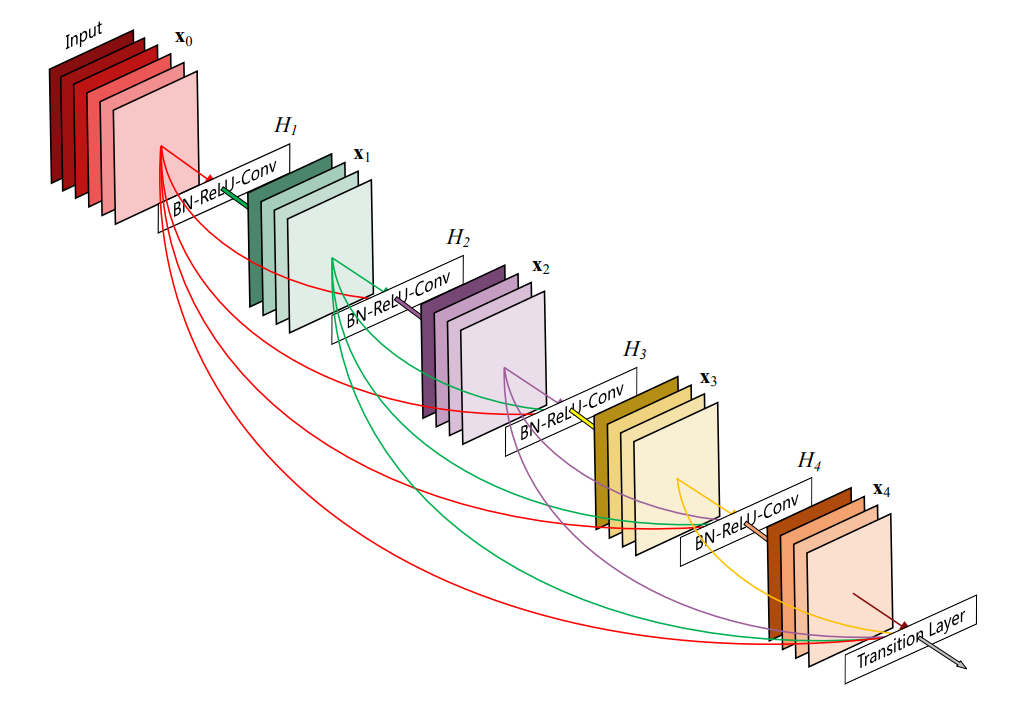
\includegraphics[width=1\textwidth]{Images/Chapter2/DenseNet.PNG}
    \caption{معماری یک بلوک
     \lr{DenseNet}\cite{huang2017densely}.}
    \label{fig:densenet_architecture}
\end{figure}






\subsection{\lr{EfficientNet}}

\lr{Tan}\cite{tan2019efficientnet} 
 و همکارانش یک معماری و روش مقیاس‌گذاری را در مدلی به نام 
 \lr{EfficientNet}
  معرفی کردند. این روش به ما امکان می‌دهد که تعداد متغیرهای مدل را به‌صورت بهینه افزایش دهیم. در این روش، برای افزایش تعداد متغیرهای مدل، سه ویژگی عمق، عرض و وضوح
   \LTRfootnote{Resolution}
  تصویر باید به‌صورت یکنواخت و با استفاده از سه ضریب ثابت افزایش پیدا کنند.

به به‌صورت مشخص، اگر بخواهیم تعداد متغیر‌های مدل را به میزان \(2^N\) برابر افزایش دهیم، می‌توانیم به‌سادگی عمق شبکه را به میزان \( \alpha^N \)، عرض شبکه را به میزان \( \beta^N \) و وضوح تصویر را به میزان \( \gamma^N \) افزایش دهیم که در آن \(\alpha\)، \(\beta\) و \(\gamma\) ضرایب ثابتی هستند که 
\autoref{eq:ch2-EffNet}
باید برای آنها برقرار باشد. این رابطه به این معناست که افزایش منابع محاسباتی به میزان \(2^N\) برابر، به توزیع متناسبی از افزایش عمق، عرض و وضوح تصویر منجر می‌شود. 

 
\begin{latin}
\begin{equation}
\label{eq:ch2-EffNet}
\begin{aligned}
\alpha \times \beta^2 \times \gamma^2 \approx 2
\end{aligned}
\end{equation}
\end{latin}

 در نتیجه پژوهش 
 \lr{Tan}
  و همکارانش، یک خانواده از مدل‌های مبتنی بر شبکه عصبی پیچشی ایجاد شد که ضمن داشتن تعداد متغیرهای بسیار کمتر، عملکرد بهتری نسبت به مدل‌های قبلی ایفا می‌کند.
 

\section{مدل‌های قطعه‌بندی در شبکه عصبی عمیق}

\subsection{\lr{U-Net}}

شبکه
 \lr{U-Net} 
 یکی از پرکاربردترین معماری‌ها در حوزه‌ی پردازش تصویر و به‌ویژه در بخش‌بندی تصاویر است که توسط
 \lr{Ronneberger}\cite{ronneberger2015u}
 و همکاران توسعه داده ‌شده است. این مدل که در اصل به‌عنوان یک شبکه عصبی پیچشی خودرمزگذار
  \LTRfootnote{Autoencoder}
   معرفی شد، به دلیل طراحی خاص خود که امکان بازیابی دقیق اطلاعات مکانی را به کمک مسیرهای  میان‌بر فراهم می‌آورد، به به‌صورت گسترده‌ای مورد استفاده قرار می‌گیرد.

ساختار \lr{U-Net} شامل دو مسیر اصلی است؛ 
مسیر اول، رمزگذار نام دارد که مسئول استخراج ویژگی‌ها و کاهش ابعاد و افزایش تعداد کانال‌ها است.
مسیر بعدی،‌رمزگشا نام دارد که وظیفه بازسازی تصویر به‌اندازه اصلی و مشخص‌کردن محل جسم را برعهده دارد که این کار را با استفاده از اطلاعات استخراج‌شده از مسیر رمزگذار انجام می‌دهد.

ساختار شبکه 
 \lr{U-Net} 
در \autoref{fig:unet_architecture} مشاهده می‌شود که مسیر رمزگذار شامل چندین مرحله از شبکه عصبی پیچشی و لایه ادغام
 \LTRfootnote{Pooling}
 است. از سوی دیگر، مسیر رمزگشا شامل افزایش ابعاد و ترکیب ویژگی‌های استخراج‌شده در مسیر رمزگذار است تا تصویر نهایی با دقت بالایی بازسازی شود. یکی از ویژگی‌های کلیدی
  \lr{U-Net}
  مسیرهای  میان‌بر بین لایه‌های رمزگذار و رمزگشا متناظر است که اطلاعات مکانی دقیق را از رمزگذار به رمزگشا منتقل می‌کند.

\begin{figure}[h]
    \centering
    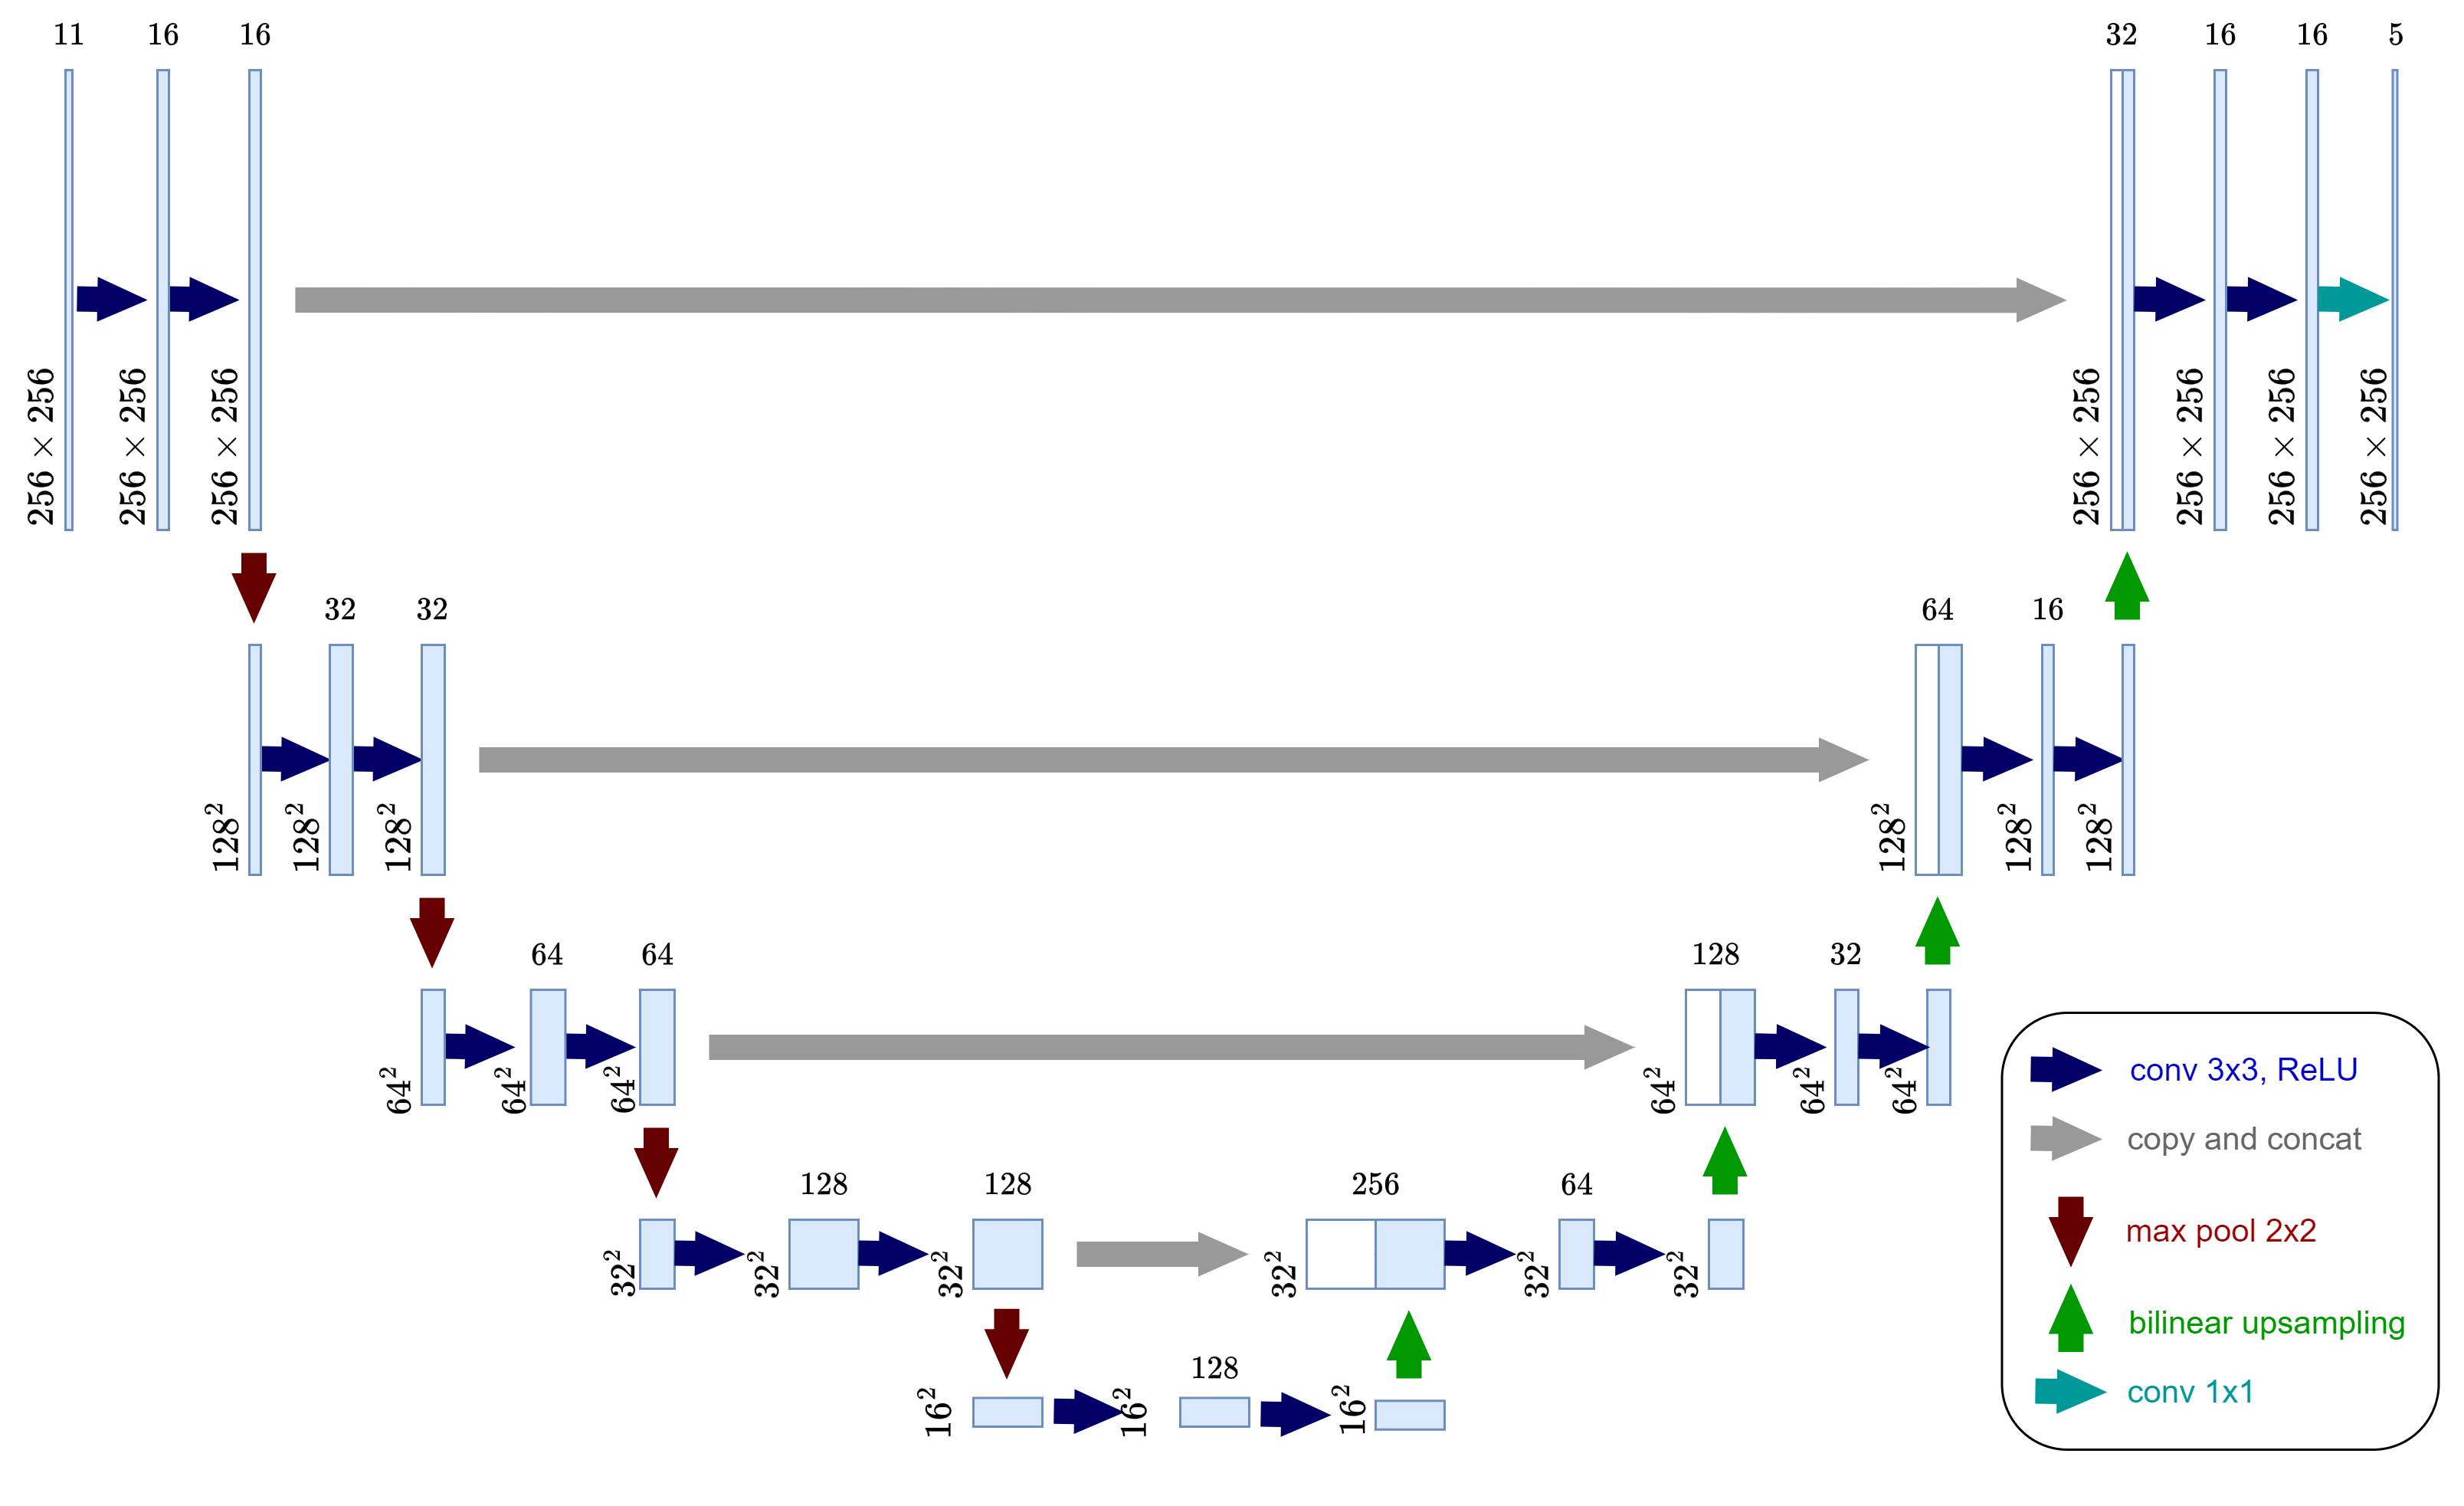
\includegraphics[width=1\textwidth]{Images/Chapter2/U-Net.drawio.png}
    \caption{ساختار شبکه
     \lr{U-Net}
      که شامل مسیر رمزگذار، رمزگشا و اتصالات میان‌بر است
    \cite{ronneberger2015u}.}
    \label{fig:unet_architecture}
\end{figure}

درحالی‌که ساختار اصلی \lr{U-Net} به‌خوبی قادر به انجام وظایف مختلف است، امکان بهبود عملکرد آن با استفاده از مدل‌های پیشرفته‌تر در بخش رمزگذار وجود دارد. به‌عنوان‌مثال، می‌توان از مدل‌هایی که در بخش‌های قبل مطرح شد،‌ مانند
 \lr{ResNet}، \lr{ResNeXt}، \lr{SENet} و \lr{EfficientNet}
  در مسیر رمزگذار
   \lr{U-Net} 
   استفاده کرد. این مدل‌ها به دلیل قابلیت‌های قدرتمند خود در استخراج ویژگی‌ها و مدیریت اطلاعات پیچیده، می‌توانند عملکرد
    \lr{U-Net} 
    را در وظایف پیچیده‌تر به به‌صورت قابل‌توجهی بهبود بخشند. 
این قابلیت به‌ویژه در مواقعی که تصاویر ورودی دارای جزئیات بسیار بالایی هستند یا نیاز به دقت بالایی در خروجی است، اهمیت بیشتری پیدا می‌کند. به همین دلیل، \lr{U-Net} با ساختار خود، یکی از انعطاف‌پذیرترین مدل‌ها برای ترکیب با معماری‌های دیگر به شمار می‌رود و به ‌به‌صورت گسترده در زمینه‌های مختلف از جمله پزشکی و بینایی ماشین مورداستفاده قرار می‌گیرد.


\section{\lr{PSPNet}}

شبکه
\lr{Pyramid Scene Parsing Network (PSPNet)}،
 که توسط
  \lr{Zhao}\cite{zhao2017pyramid}
   و همکاران  معرفی شده است، یک مدل مبتنی‌بر شبکه عصبی پیچشی برای وظیفه طبقه‌بندی است. یکی از نقاط قوت اصلی
    \lr{PSPNet}،
      توانایی آن برای استخراج ویژگی‌ها با مقایاس‌های متفاوت از طریق لایه ادغام است. این ویژگی به مدل اجازه می‌دهد که با در نظر گرفتن اطلاعات از نواحی مختلف تصویر در مقیاس‌های متفاوت، پیش‌بینی‌های پیکسلی دقیق‌تری ارائه دهد.

\lr{PSPNet}
 با استفاده از انواع رمزگذار که در بخش قبل مطرح شد به عنوان بلوک استخراج ویژگی، ساختار خود را ایجاد می‌کند. این معماری برای رفع چالش‌های رایج در طبقه‌بندی تصاویر، مانند دسته‌بندی‌های گیج‌کننده و اشیاء کوچک که به سختی دیده می‌شوند، طراحی شده است و مشکلاتی که در ساختارهای قبلی منجر به طبقه‌بندی نادرست می‌شوند را بهبود می‌بخشد.
\autoref{fig:pspnet}
ساختار این شبکه را نشان می‌دهد که در گام نخست با استفاده از رمزگذار،‌ نقشه ویژگی‌ها استخراج شده است و در ادامه با استفاده از بلوک ادغام هرمی، ویژگی‌ها با ابعاد متفاوت استخراح می‌شوند، سپس ویژگی‌ها به یکدیگر الحاق شده و در انتها ابعاد ویژگی‌ها به ابعاد اصلی تصویر تبدیل می‌شوند تا پیش‌بینی نهایی بدست آید.

\begin{figure}[h]
\centering
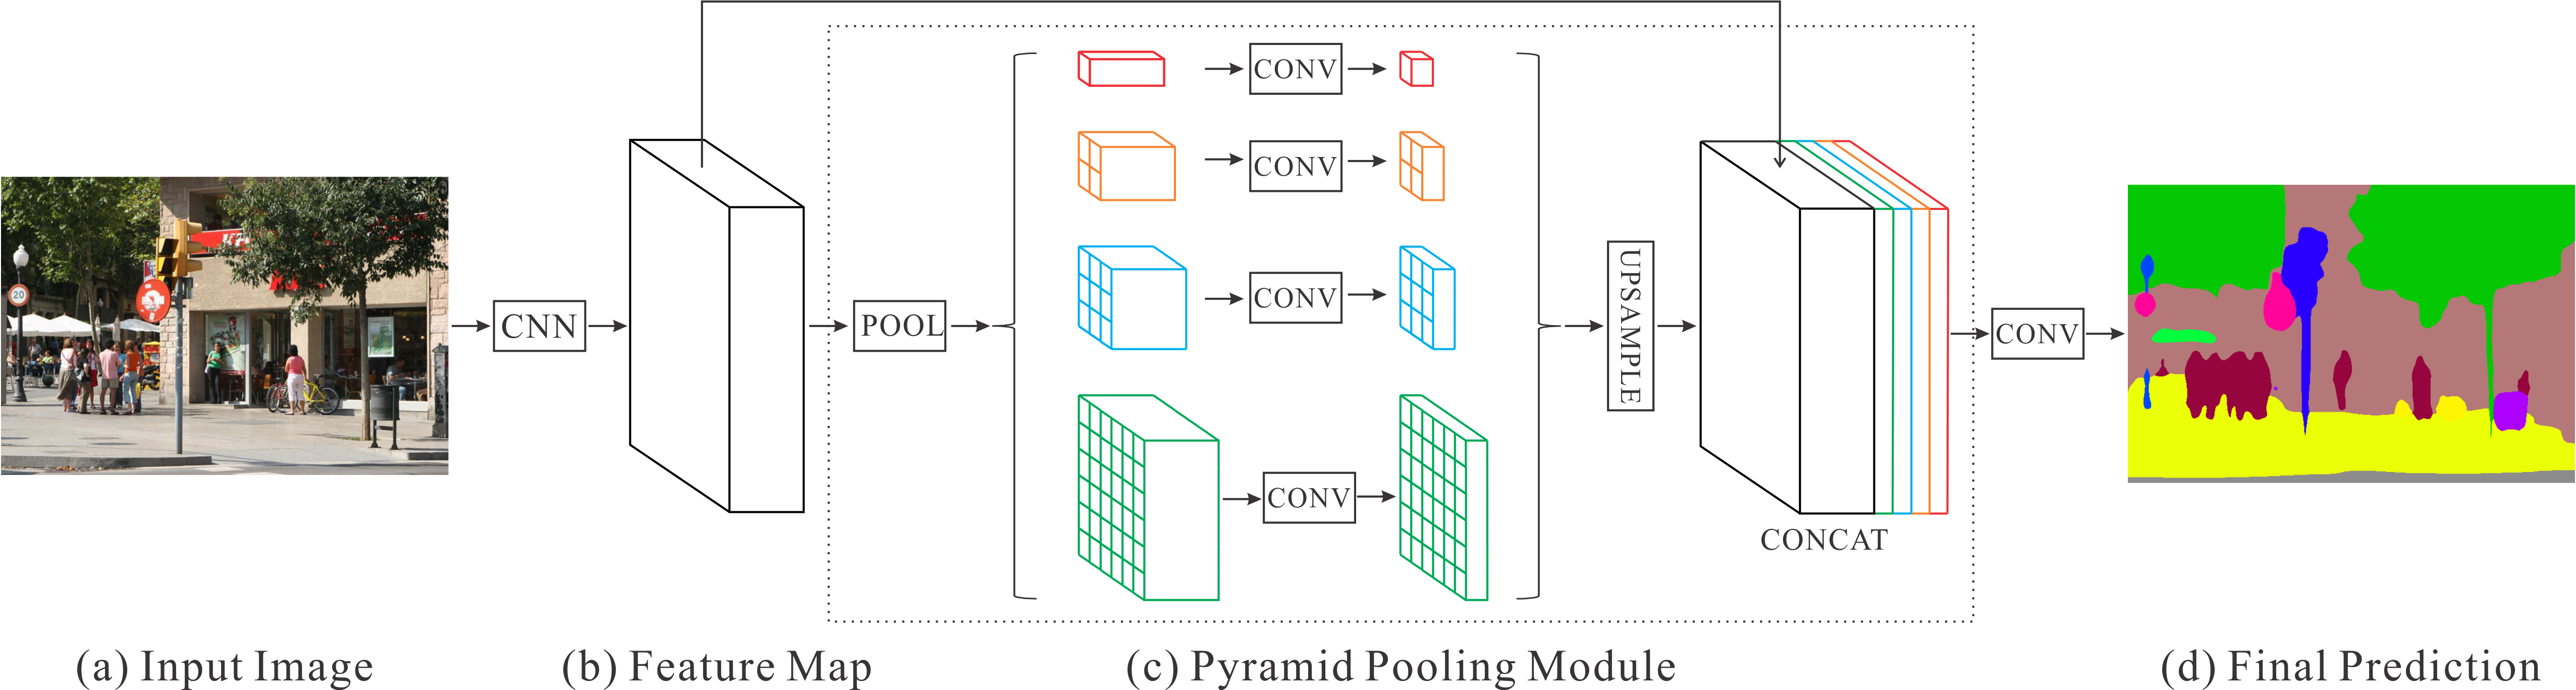
\includegraphics[width=1.0\linewidth]{Images/Chapter2/PSPNet}
\caption{ساختار شبکه \lr{PSPNet}
\cite{zhao2017pyramid}}
\label{fig:pspnet}
\end{figure}

\section{پس‌پردازش}
\label{ch2-post-process}
پس‌پردازش پیشنهادی در این پژوهش، به‌منظور بهبود عملکرد مدل قطعه‌بندی، توسعه داده شده است.
\autoref{fig:ct2-3d}
یک نمونه تصویر سی‌تی‌اسکن را نشان می‌دهد. به همان‌ صورت که در این تصویر مشخص است،‌ حاشیه سیاه برش‌ها، شامل هیچ اندامی نیست و بدیهی است که هیچ ضایعه خونریزی در این نواحی یافت نخواهد شد، بنابراین، با‌توجه‌‌به اینکه یکای 
 \lr{Hounsfield}
 این نواحی بسیار از مقدار آن در بافت مغز متفاوت است، بنابراین روش آستانه‌گذاری روی برش‌ها اعمال شد که آستانه مربوطه از روی 
\autoref{fig: ch2-slice hist lim}،
به‌گونه‌ای انتخاب شد که نواحی شامل بافت مغز از نواحی فاقد اندام جدا شوند.
\autoref{fig:ch2-post-process-mask}
لایه‌های پس‌پردازش استخراج‌شده با روش آستانه‌گذاری را برای برش‌های متفاوت نشان می‌دهد. این لایه‌ها پس از استخراج، در مرحله تصمیم‌گیری مدل قطعه‌بندی استفاده می‌شوند. روش استفاده از این لایه‌ها به‌گونه‌ای است که احتمال هرگونه پیش‌بینی موجود در نواحی سیاه از تصویر را برابر
$ 0$ 
قرار می‌دهد و باعث می‌شود تا نیاز به آموزش لایه‌های مدل قطعه‌بندی  در این نواحی لازم نباشد.




\begin{figure}[h]
\centering
\includegraphics[width=1.0\linewidth]{"Images/Chapter2/post-process mask"}
\caption{نمونه لایه‌های پس‌پردازش استخراج شده از برش‌های بیمار}
\label{fig:ch2-post-process-mask}
\end{figure}




\section{روش پیشنهادی}
هدف اصلی در این پژوهش،‌ بهبود عملکرد مدل‌های قطعه‌بندی در تصاویر سی‌تی‌اسکن بوده به‌گونه‌ای که این روش به‌صورت عام، امکان پیاده‌سازی روی مدل‌های قطعه‌بندی را داشته باشد. به‌منظور توسعه این روش،‌ ناترازی داده‌ها،‌ به‌عنوان یکی از اصلی‌ترین مشکلات در پردازش تصاویر سه‌بعدی پزشکی و سی‌تی‌اسکن موردمطالعه قرار گرفت.

ناترازی در داده‌های سی‌تی‌اسکن، خصوصاً برای پردازش خونریزی درون‌جمجمه‌ای، می‌تواند در سه سطح بیمار‌محور، برش‌محور و پیکسل‌محور رخ دهد که در مجموعه‌داده موجود،‌ این ناترازی تنها در دو سطح برش‌محور و پیکسل‌محور رخ‌داده است. 
\autoref{fig: ch2-patient distrbiution}
پراکندگی داده را به‌صورت بیمارمحور و 
\autoref{fig: ch2-slice distribution}
پراکندگی داده را به‌صورت برش‌محور نشان می‌دهد که ناترازی در سطح برش، بسیار شدید است. 
پراکندگی پیکسل‌های دارای خونریزی نیز در این مجموعه‌داده، به‌گونه‌ای است که در برش‌هایی که ضایعه خونریزی وجود دارد، تعداد پیکسل‌های دارای خونریزی، در حدود 2000 پیکسل است که این مقدار در برابر تعداد پیکسل‌های کل برش که برابر 
$2^{18}$
پیکسل است،‌ نشان‌دهنده شدت بیشتر ناترازی در سطح پیکسل است.

برای کاهش مشکل ناترازی در سطح برش، یک روش دومرحله‌ای، توسعه داده‌ شد که به‌موجب آن،‌ در گام نخست برش‌های سی‌تی‌اسکن طبقه‌بندی خواهند شد تا وجود ضایعه تشخیص داده ‌شود و در گام بعدی،‌ برش‌هایی که دارای بیماری پیش‌بینی شده‌اند،‌ به یک شبکه قطعه‌بندی ارسال می‌شوند تا مراحل قطعه‌بندی در این برش‌ها طی شود.
استفاده از این روش برای پردازش تصاویر سی‌تی‌اسکن،‌این مزیت را دارد که با حذف برش‌های سالم از فرایند تصمیم‌گیری، باعث کاهش تعداد پیکسل‌هایی می‌شود که به‌صورت اشتباه،‌ به‌عنوان پیکسل‌های دارای ضایعه خونریزی در نظر گرفته شده‌اند. نکته حائز اهمیت درمورد این روش این است که تمام خطاهایی که در مدل طبقه‌بندی رخ بدهند، مستقیماً  در عملکرد مدل قطعه‌بندی تأثیر  می‌گذارند خصوصاً  اگر برشی که دارای خونریزی بوده، به‌عنوان برش سالم در نظر گرفته شود؛ بنابراین باید توجه داشت تا آستانه تصمیم‌گیری در این روش به‌گونه‌ای انتخاب شود تا تعداد برش‌هایی که واقعاً سالم نیستند، اما سالم تشخیص‌ داده می‌شوند به حداقل مقدار خود برسد. حد بالای پیشنهادی برای این آستانه به‌گونه‌ای است که به‌موجب آن، تمام سی‌تی‌اسکن‌های دارای خونریزی  موجود در مجموعه‌داده به‌درستی تشخیص داده ‌شوند (تشخیص بیمار‌محور). 

استفاده از روش پس‌پردازش مذکور در 
\autoref{ch2-post-process}،
	باعث می‌شود تا ناترازی در سطح پیکسل تا حد خوبی کاهش پیدا کند و به‌موجب آن فرایند آموزش مدل، بیشتر معطوف به شناسایی نواحی دارای خونریزی شود تا اینکه یک قسمت از فرایند آموزش مدل صرف این شود تا نواحی خارج از جمجمه شناسایی شود. این پس‌پردازش به ما این امکان را می‌دهد تا با کاهش میزان آستانه تصمیم، تعداد پیکسل‌هایی که به‌درستی درون جمجمه شناسایی می‌شوند را افزایش دهیم. پس‌پردازش مذکور در پژوهش، به‌صورت مجتمع در فرایند آموزش استفاده شده است.
	\begin{figure}[h]
\centering
\includegraphics[height=0.5\textheight]{"Images/Chapter2/block diagram of 2 step .drawio"}
\caption{روندنمای روش پیشنهادی در این پژوهش}
\label{fig:ch2-block-diagram-of-2-step}
\end{figure}

\autoref{fig:ch2-block-diagram-of-2-step}
روندنمای روش پیشنهادی و پس‌پردازش را به‌منظور بررسی برش‌های خونریزی نشان می‌دهد که در این پردازش استفاده شده‌است. همانطور که از این روند‌نما مشخص است، این روند بستگی به مدل طبقه‌بندی و قطعه‌بندی مورد استفاده ندارد و می‌توان از هر مدلی در این روند استفاده کرد که این مسئله باعث افزایش قابلیت توسعه و نگهداری نرم‌افزارهایی می‌شود که بر پایه این روند توسعه داده‌ شده‌اند.

\section{آموزش و تصمیم‌گیری}

\subsection{طبقه‌بندی}

گام نخست در این پژوهش، آموزش یک مدل طبقه‌بندی مناسب به‌منظور استفاده در روش دومرحله‌ای است که به‌موجب آن یک جستجوی شبکه‌ای 
\LTRfootnote{Grid Search}
با استفاده از مدل 
\lr{ResNet 50}
انجام شد که وزن‌ اولیه این مدل با استفاده از روش انتقال یادگیری به روی مجموعه‌داده 
\lr{ImageNet}
\cite{deng2009imagenet}
انتخاب شده است. در این جستجوی شبکه‌ای،‌ باتوجه‌به چالش‌ ناترازی مجموعه‌داده، از تابع هزینه 
\lr{Cross Entropy}
وزن‌دار استفاده شد و همچنین با استفاده از روش افزایش مصنوعی داده، جاگذاری داده
\LTRfootnote{Bootstrap}
و کاهش داده غالب در ضرایب متفاوت استفاده شد تا بهترین نتیجه ممکن برای مدل طبقه‌بندی یافت شود. 
\autoref{table:ch2-grid-values}
نمایش‌دهنده مقادیر مورداستفاده در جستجوی شبکه‌ای است. در این جستجوی شبکه‌ای، کاهش داده غالب باتوجه‌به توزیع برش‌های دارای خونریزی که در 
\autoref{fig:ch2-slice-hist}
نمایش‌داده‌شده است انجام شده تا داده‌هایی که کمترین تأثیر  را در آموزش دارند،‌ با احتمال بیشتری کنار گذاشته شوند و ضریبی که در جدول 
\autoref{table:ch2-grid-values}
برای این روش اعلام شده،‌ به این معنی است که نسبت برش‌های بیمار به برش‌های سالم پس از اعمال این روش، برابر ضریب اعلامی خواهد شد.
در ادامه افزایش مصنوعی داده و جاگذاری داده نیز‌ تنها به روی برش‌هایی با تشخیص خونریزی درون‌جمجمه‌ای صورت پذیرفته و تا متناسب  با پراکندگی برش‌های دارای خونریزی، افزایش این داده‌ها صورت پذیرد که در 
\autoref{fig:ch2-slice-hist}
توزیع این داده‌ها نمایش‌داده‌شده است و پس از اعمال این روش‌ها، تعداد برش‌های بیمار در ضریب اعلام شده ضرب شده است. باید توجه داشت که در جستجوی شبکه‌ای ابتدا  افزایش مصنوعی داده و جاگذاری داده اعمال شده و پس از آن کاهش داده غالب روی مجموعه‌داده اعمال شده است.
در آموزش مدل طبقه‌بندی، به علت وجود تعداد کم داده‌های دارای خونریزی و احتمال بیش‌برازش\LTRfootnote{Overfit}،
از روش 
\lr{5-fold-cross-validation}
استفاده شد. در گام نخست از استفاده از این روش، یک زیرمجموعه ارزیابی
\LTRfootnote{Test}
که 20 درصد از کل مجموعه‌داده می‌باشد، انتخاب شده ‌است و پس از آن روی باقی مجموعه‌داده عملیات
\lr{5-fold-cross-validation}
را برای آموزش مدل انجام شده است؛ در انتها پس از فرایند آموزش، تنظیم متغیرهای تصمیم‌گیری‌ مدل‌های به‌دست‌آمده روی مجموعه‌داده ارزیابی انجام شده و سازوکار تصمیم‌گیری شورایی
\LTRfootnote{Voting}
نهایی شده است که این سازوکار در 
\autoref{ch2-decision-policy}
توضیح داده شده است.
در انتها مدل پیشنهادی روی مجموعه‌داده ارزیابی آزمایش شده است. استفاده از این روش باعث می‌شود تا از عملکرد مدل و مقاوم‌بودن آن اطمینان حاصل شود. به‌منظور اطمینان از اینکه متغیرهای به‌دست‌آمده در عملیات جستجوی شبکه‌ای،‌ در بهبود عملکرد مدل‌های شبکه عصبی تأثیرگذار است، مدل‌های 
\lr{VGG16}،\lr{MobileNet-V2} و \lr{Inception‌-V3}
نیز با بهترین تنظیمات به‌دست‌آمده روی 
\lr{ResNet50} 
آموزش داده شد.

\begin{table}[h]
\centering
\caption{ضرایب مورد استفاده در جستجوی شبکه‌ای}
\label{table:ch2-grid-values}
\resizebox{\textwidth}{!}{%
\begin{tabular}{llll}
\textbf{روش}                       & \textbf{ضریب اول} & \textbf{ضریب دوم} & \textbf{ضریب سوم} \\ \hline
افزایش مصنوعی داده                 & $2$               & $2.5$             & $3.3$             \\
جاگذاری داده                      & $2$               & $2.5$             & $3.3$             \\
کاهش داده غالب                     & $1$               & $2$               & $3$               \\
افزایش وزن داده مثبت در تابع هزینه & $2$               & $4$               & $6$               \\
کاهش وزن داده منفی در تابع هزینه   & $0.5$             & $0.25$            & $-$               
\end{tabular}%
}
\end{table}

\subsection{قطعه‌بندی}
در این پژوهش،‌ مدل شبکه عصبی عمیق 
\lr{U-Net}
به‌عنوان ساختار اصلی برای آموزش وظیفه قطعه‌بندی در نظر گرفته شده است که وزن‌ اولیه این مدل با استفاده از روش انتقال یادگیری به روی مجموعه‌داده 
\lr{ImageNet}
\cite{deng2009imagenet}
انتخاب شده است. به‌منظور آموزش این مدل یک جستجوی شبکه‌ای جامع روی مجموعه‌داده انجام شد. متناسب با نتایجی که به روی وظیفه طبقه‌بندی به‌دست‌آمده، استفاده از روش‌هایی مثل کاهش داده غالب و جاگذاری داده تأثیر  مناسبی روی نتایج نداشته است؛ بنابراین این دو روش در جستجوی شبکه‌ای مدل قطعه‌بندی استفاده نشده است. در آموزش مدل قطعه‌بندی به روش جستجوی شبکه‌ای، از روش افزایش مصنوعی داده با ضرایب 
$3$، $4$، $5$ و $6$
به همراه انواع مختلف توابع هزینه شامل 
\lr{Dice}، \lr{Tversky}، \lr{Focal Tversky}، \lr{Focal}،  \lr{Cross-entropy} و
\lr{Cross-entropy}
وزن‌دار با وزن‌های 10، 100،‌ 200، 500 و 1000 برای پیکسل‌های مثبت و انواع مختلف رمزگذار در ساختار شبکه 
\lr{U-Net}
با ابعاد متفاوت شامل 
\lr{ResNet}، \lr{ResNeXt}، \lr{SE-ResNeXt}, \lr{EfficientNet}
و 
\lr{DenseNet}
استفاده شده است.

در مراحل آموزش مدل قطعه‌بندی، داده ارزیابی ابتدا از مدل شورایی طبقه‌بندی عبور داده شد و تمام برش‌هایی که در این مدل دارای خونریزی درون‌جمجمه‌ای تشخیص داده شده‌اند،‌ طبق روندنمای 
\autoref{fig:ch2-block-diagram-of-2-step}
به مدل قطعه‌بندی ارسال شدند تا برش‌ها قطعه‌بندی شوند.
در گام آخر، یک سازوکار تصمیم‌گیری شورایی که در 
\autoref{ch2-decision-policy}
توضیح داده شده است، 
برای قطعه‌بندی برش‌ها استفاده شد تا پیش‌بینی مدل‌های متفاوت مورداستفاده قرار گیرد.



\subsection{سازوکار تصمیم‌گیری شورایی}
\label{ch2-decision-policy}
استفاده از روش
\lr{5-fold-cross-validation}
برای ارزیابی مدل‌های شبکه‌ عصبی،‌ می‌تواند با یک سازوکار شورایی در لایه تصمیم‌گیری همراه شود که به‌موجب آن اثر بیش‌برازش روی مجموعه‌داده کاهش پیدا می‌کند. در این پژوهش،‌ یک روش شورایی ساده برای وظیفه طبقه‌بندی پیشنهاد شده است که به‌موجب آن، از پیش‌بینی احتمالاتی تمام مدل‌ها میانگین گرفته می‌شود و در انتها آستانه‌گذاری روی این میانگین اعمال می‌شود. در ادامه برای وظیفه قطعه‌بندی،‌ مراحل به‌گونه‌ای است که ابتدا برای هر مدل آستانه‌گذاری انجام شده و سپس بین آرای هر مدل رأی گرفته می‌شود 
\autoref{fig:decisionmaking}،
عملکرد این روش را به‌صورت روند‌نما مشخ می‌کند.


\begin{figure}[h!]
		\centering % <-- added
		\begin{subfigure}{0.49\textwidth}
			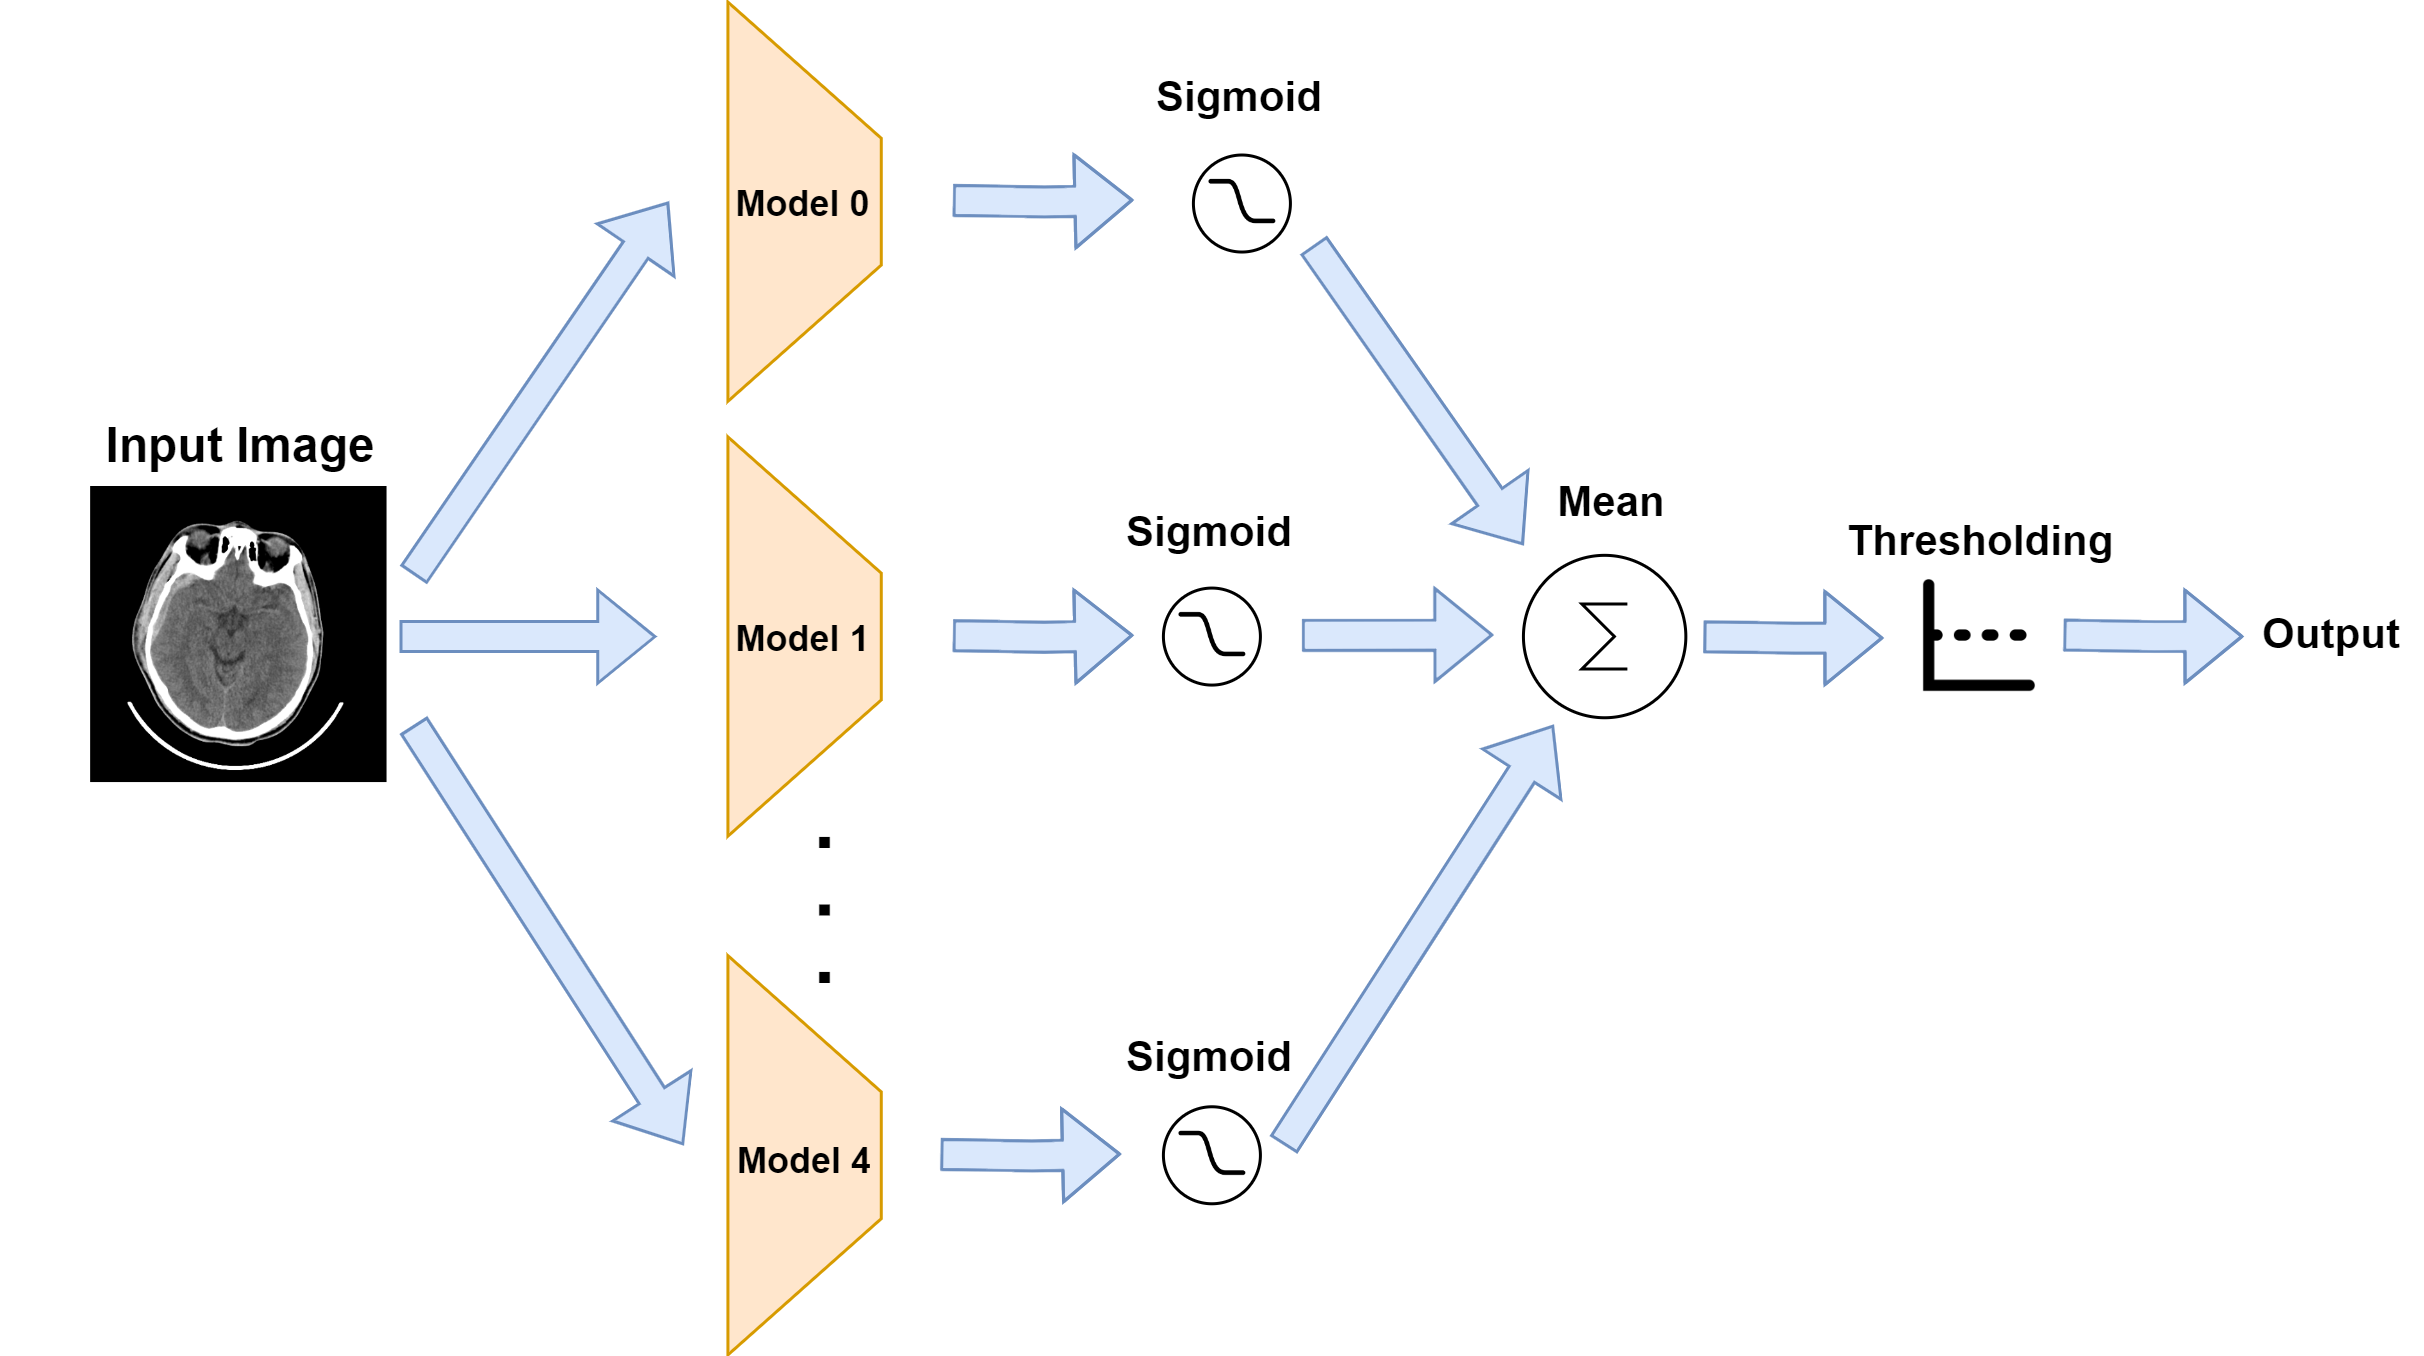
\includegraphics[width=\linewidth]{Images/Chapter2/decision_making.drawio}
			\caption{سازوکار طبقه‌بندی}
			\label{f61}
		\end{subfigure}\hfil % <-- 
		\begin{subfigure}{0.49\textwidth}
			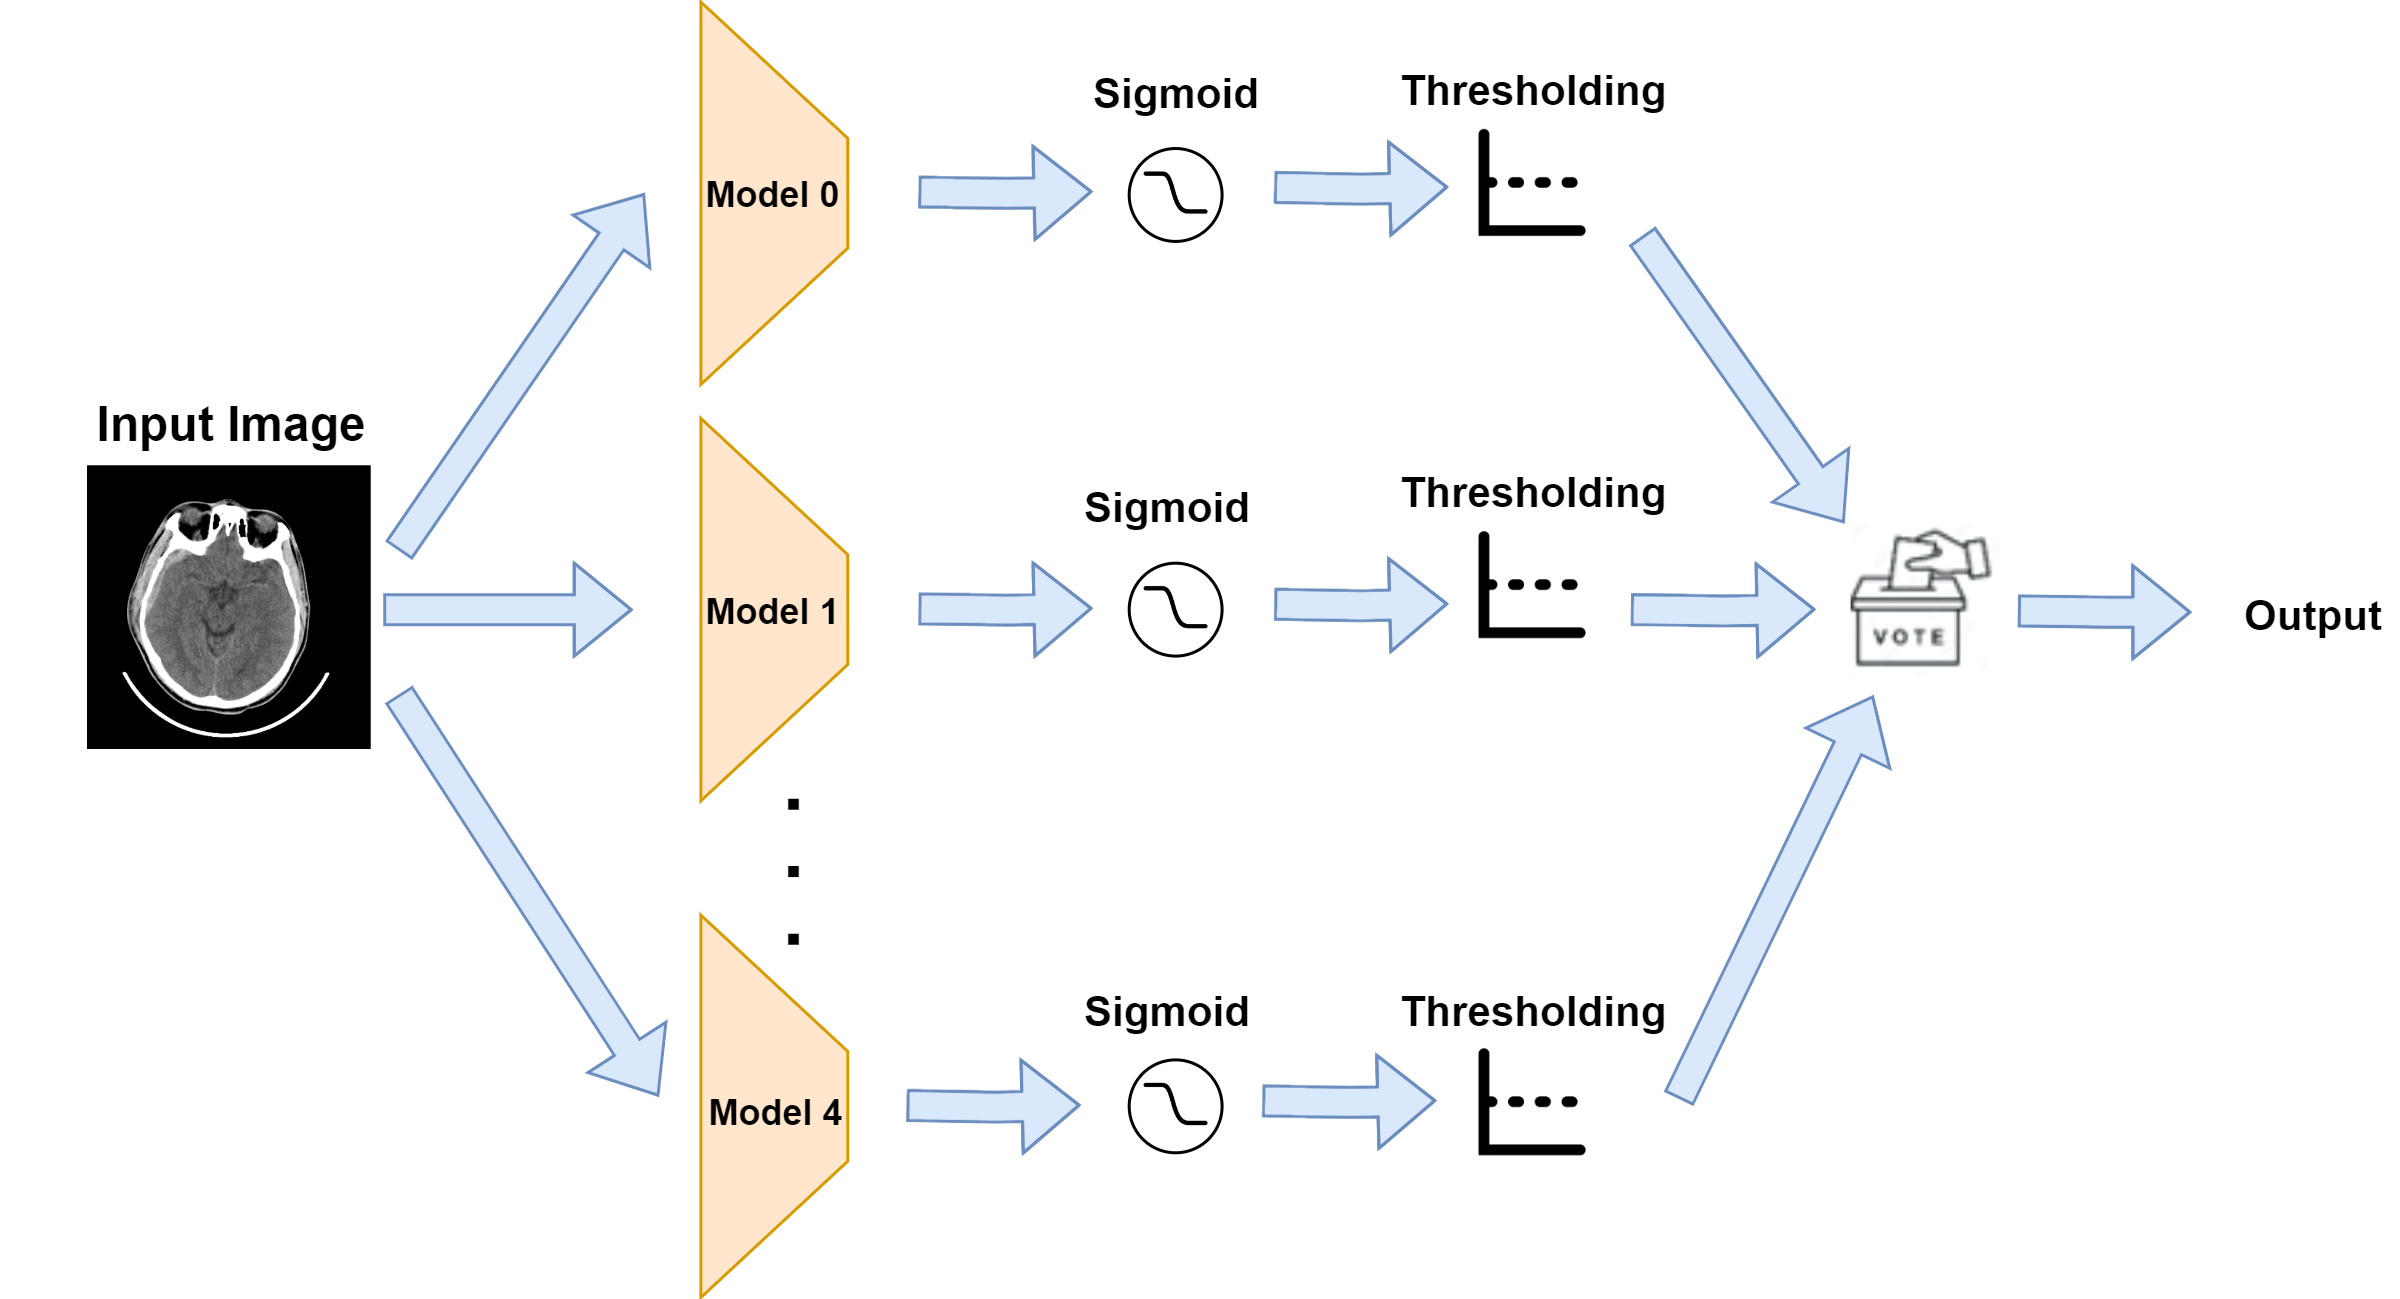
\includegraphics[width=\linewidth]{Images/Chapter2/decision_making_seg.drawio}
			\caption{سازوکار قطعه‌بندی}
			\label{f62}
		\end{subfigure}\hfil % <-- added

		\caption{سازوکار تصمیم‌گیری شورایی}
		\label{fig:decisionmaking}
\end{figure}


\chapter{نتایج}
\section{معیارهای ارزیابی در یادگیری عمیق}

در این بخش، به بررسی معیارهای مختلفی که برای ارزیابی مدل‌های یادگیری عمیق استفاده می‌شوند، می‌پردازیم. این معیارها شامل \lr{Sensitivity}، \lr{Specificity}، \lr{Precision}، \lr{F1 Score}، \lr{Accuracy}، \lr{Intersection over Union (IoU)} و ضریب \lr{Dice} است.

قبل از پرداختن به تعریف این معیارها، ابتدا به تعریف چهار مفهوم اساسی می‌پردازیم که در فرمول‌های ارزیابی به ‌کار می‌روند:

\begin{itemize}
    \item \textbf{\lr{TP} \lr{(True Positives)}}: تعداد نمونه‌های مثبت که به‌درستی به‌عنوان مثبت دسته‌بندی شده‌اند.
    \item \textbf{\lr{FP} \lr{(False Positives)}}: تعداد نمونه‌های منفی که به‌اشتباه به‌عنوان مثبت دسته‌بندی شده‌اند.
    \item \textbf{\lr{TN} \lr{(True Negatives)}}: تعداد نمونه‌های منفی که به‌درستی به‌عنوان منفی دسته‌بندی شده‌اند.
    \item \textbf{\lr{FN} \lr{(False Negatives)}}: تعداد نمونه‌های مثبت که به‌اشتباه به‌عنوان منفی دسته‌بندی شده‌اند.
\end{itemize}

\subsection{\lr{Sensitivity}}

\lr{Sensitivity}
که با نام نرخ تشخیص صحیح نیز شناخته می‌شود، معیاری برای ارزیابی توانایی مدل در تشخیص صحیح نمونه‌های مثبت است. فرمول این معیار در \autoref{eq:sensitivity} مشخص شده است.

\begin{latin}
\begin{equation}
\label{eq:sensitivity}
\text{Sensitivity} = \frac{TP}{TP + FN}
\end{equation}
\end{latin}

\subsection{\lr{Specificity}}

\lr{Specificity}
، معیاری است که نشان‌دهنده توانایی مدل در شناسایی صحیح نمونه‌های منفی است. فرمول این معیار در \autoref{eq:specificity} مشخص شده است.

\begin{latin}
\begin{equation}
\label{eq:specificity}
\text{Specificity} = \frac{TN}{TN + FP}
\end{equation}
\end{latin}

\subsection{\lr{Precision}}

\lr{Precision}،
 معیاری برای ارزیابی میزان درستی دسته‌بندی نمونه‌های مثبت است.به‌عبارت‌دیگر،
  \lr{Precision}
   نسبت نمونه‌های مثبت درست دسته‌بندی شده به تمام نمونه‌های پیش‌بینی‌شده به‌عنوان مثبت است. فرمول آن در
    \autoref{eq:precision}
     مشخص شده است.

\begin{latin}
\begin{equation}
\label{eq:precision}
\text{Precision} = \frac{TP}{TP + FP}
\end{equation}
\end{latin}

\subsection{\lr{F1 Score}}

\lr{F1 Score}، میانگین موزون \lr{Precision} و \lr{Sensitivity} است که تعادلی بین این دو معیار ایجاد می‌کند. این امتیاز به‌ویژه در مواردی که تعادل بین \lr{Precision} و \lr{Sensitivity} اهمیت دارد، مورداستفاده قرار می‌گیرد. فرمول \lr{F1 Score} در \autoref{eq:f1_score} مشخص شده است.

\begin{latin}
\begin{equation}
\label{eq:f1_score}
\text{F1 Score} = 2 \times \frac{\text{Precision} \times \text{Sensitivity}}{\text{Precision} + \text{Sensitivity}}
\end{equation}
\end{latin}

\subsection{\lr{Accuracy}}

\lr{Accuracy}، نسبت نمونه‌هایی است که به‌درستی دسته‌بندی شده‌اند به تمام نمونه‌ها. این معیار نشان‌دهنده عملکرد کلی مدل است و فرمول آن در \autoref{eq:accuracy} مشخص شده است.

\begin{latin}
\begin{equation}
\label{eq:accuracy}
\text{Accuracy} = \frac{TP + TN}{TP + TN + FP + FN}
\end{equation}
\end{latin}

\subsection{\lr{Intersection over Union (IoU)}}

\lr{Intersection over Union}
 که به‌عنوان \lr{Jaccard Index} نیز شناخته می‌شود، معیاری است که برای ارزیابی همپوشانی بین دو مجموعه، به‌ویژه در مسائل بخش‌بندی تصویر، استفاده می‌شود. فرمول \lr{IoU} در \autoref{eq:iou} مشخص شده است.

\begin{latin}
\begin{equation}
\label{eq:iou}
\text{IoU} = \frac{|A \cap B|}{|A \cup B|} = \frac{TP}{TP + FP + FN}
\end{equation}
\end{latin}

\subsection{ضریب
\lr{Dice}}

ضریب \lr{Dice}، مشابه \lr{IoU} است؛ اما وزن بیشتری به ناحیه اشتراک می‌دهد و در مسائل بخش‌بندی تصویر بسیار مورداستفاده قرار می‌گیرد. فرمول ضریب \lr{Dice} در \autoref{eq:dice} مشخص شده است.

\begin{latin}
\begin{equation}
\label{eq:dice}
\text{Dice Coefficient} = \frac{2 \times |A \cap B|}{|A| + |B|} = \frac{2 \times TP}{2 \times TP + FP + FN}
\end{equation}
\end{latin}

\section{نتایج طبقه‌بندی}

در این بخش، نتایج حاصل از مدل‌های طبقه‌بندی خونریزی درون‌جمجمه‌ای در تصاویر سی‌تی‌اسکن، بررسی و تحلیل شده‌اند. تمرکز اصلی آموزش مدر طبقه‌بندی بر روی بهینه‌سازی فراپارامترها برای مدل
 \lr{ResNet50}
  بوده است که بهبود قابل‌توجهی در عملکرد مدل به‌ویژه در معیار \lr{Sensitivity}
   به ‌همراه داشته است. بهترین نتایج به‌دست‌آمده در جستجوی شبکه‌ای زمانی حاصل می‌شود که ضریب افزایش مصنوعی داده برابر 
   $3.3$
و وزن تابع خطا
\lr{Cross-entropy}
برای برش‌های مثبت برابر 4 و برای برش‌های منفی برابر 1 است.

\subsection{نتایج برش‌محور }
پس از آموزش مدل طبقه‌بندی برای تمام 
\lr{Fold}ها،
نمودار امتیاز
\lr{F1}
نسبت‌ به آستانه‌های متفاوت رسم شد و در گام بعدی میانگین این نمودارها محاسبه شد. در انتها بهترین آستانه روی میانگین این نمودار‌ها محاسبه شده و در محاسبه معیارهای مربوط به زیرمجموعه ارزیابی استفاده شده است.
 \autoref{tab:slice_level_results}
  نتایج به‌دست‌آمده از آموزش مدل‌های \lr{ResNet50} و سازوکار شورا برای طبقه‌بندی برش‌محور نشان می‌دهد. همان‌طور که در جدول مشاهده می‌شود، بهترین نتایج در
 \lr{Fold 0}
  به‌دست‌آمده است که امتیاز 
  \lr{F1}
   برابر با
  $0.62$
 را نشان می‌دهد. این نشان‌دهنده این است که توزیع داده‌ها در مجموعه‌های آموزشی و اعتبارسنجی این 
 \lr{Fold}
  بیشتر شبیه به مجموعه آزمون است. در مقابل، 
  \lr{Fold 4}
   کمترین نتایج را به‌دست‌آورده، درحالی‌که نتایج مراحل دیگر با هم بیشتر هم‌خوانی دارند. نتایج به‌دست‌آمده از روش شورایی، در مقایسه با نتایج گزارش‌شده توسط
   \lr{Hssayeni}\cite{hssayeni2020intracranial}
   و همکاران، در معیار
   \lr{Sensitivity}
3 درصد ضعیف‌تر عمل کرده ‌است اما در معیار
\lr{Specifity}
41 درصد بهتر عمل کرده است. مقایسه این نتایج نشان می‌دهد که مدل پیشنهادی در این پژوهش، به‌صورت نسبی همان قدر که در تشخیص برش‌هایی که خونریزی درون‌جمجمه‌ای دارند درست عمل می‌کند، در تشخیص برش‌هایی که سالم هستند نیز درست عمل می‌‌کند اما 
\lr{Hssayeni}
و همکاران در تشخیص برش‌های سالم که تعداد آنها نیز بسیار زیاد هست،‌ ضعیف عمل کرده‌اند و 50درصد از این برش‌ها را دارای خونریزی درون‌جمجمه‌ای تشخیص داده‌اند. نکته‌ای که در مورد پژوهش آنها وجود دارد،‌ عدم ارائه بقیه معیارهای ارزیابی مدل است که تحلیل و مقایسه‌ بیشتر این پژوهش را دشوار می‌سازد.
پژوهش بعدی که در زمینه طبقه‌بندی برش‌های خونریزی درون‌جمجمه‌ای با استفاده از انتقال یادگیری عمل کرده است، مربوط به 
\lr{Neethi}\cite{neethi2022stroke}
است که از مدل 
\lr{ResNet 50} 
استفاده کرده‌اند. این پژوهش در معیار
\lr{Precision}
20 درصد و در معیار امتیاز
\lr{F1}
3 درصد بهتر عمل کرده ‌است اما در معیار 
\lr{Sensitivity}
مدل آنها 18 درصد ضعیف‌تر و در معیار 
\lr{Accuracy}
مدل آنها 37 درصد ضعیف‌تر عمل کرده است. در تحلیل نتایج به‌دست‌آمده، از‌آنجایی‌که در زمینه پزشکی، تشخیص اشتباه یک نمونه دارای بیماری،‌ می‌تواند منجر به حوادث جبران‌ناپذیر شود، معیار 
\lr{Sensitivity}
مهم‌تر از معیار 
\lr{Precision}
است؛ باتوجه‌به این نکته،‌ مدل پیشنهادی ما توانسته اختلاف بسیار زیادی در این معیار ایجاد کند. از طرف دیگر با‌توجه‌به عدد 
\lr{Accuracy}
گزارش شده، مشخص است که مدل پیشنهادی 
\lr{Neethi}
تنها نیمی از برش‌های تمام مجموعه‌داده را درست تشخیص داده که نشان‌دهنده تعداد خیلی کم 
\lr{TN}
و مقدار کم 
\lr{Specificity}
است که در پژوهش آنها گزارش نشده است. نکته‌ای که باید توجه داشت این است که مدل‌های استفاده شده در هر دو پژوهش یکسان است و تنها فراپارامتر‌های پیشنهادی ما باعث بهبود عملکرد مدل شده است.


% Please add the following required packages to your document preamble:
% \usepackage{graphicx}
\begin{table}[h]
\centering
\caption{نتایج برش‌محور مدل \lr{ResNet50}
برای آستانه تصمیم‌گیری
$0.27$}
\label{tab:slice_level_results}
\resizebox{\textwidth}{!}{%
\begin{tabular}{llllll}
\hline
\multicolumn{1}{c}{\textbf{مدل}}           & \textbf{\lr{Sensitivity}} & \textbf{\lr{Specificity}} & \textbf{\lr{Precision}} & \textbf{\lr{F1}}   & \textbf{\lr{Accuracy}} \\ \hline
\lr{ResNet50 Fold 0}        & $0.78$            & $0.93$             & $0.51$         & $0.62$ & $0.91$    \\
\lr{ResNet50 Fold 1}        & $0.68$            & $0.90$             & $0.38$         & $0.49$ & $0.88$    \\
\lr{ResNet50 Fold 2}        & $0.60$            & $0.89$             & $0.33$         & $0.42$ & $0.86$    \\
\lr{ResNet50 Fold 3}        & $0.86$            & $0.89$             & $0.41$         & $0.55$ & $0.89$    \\
\lr{ResNet50 Fold 4}        & $0.32$            & $\mathbf{0.96}$             & $0.42$         & $0.36$ & $0.90$    \\ \hline
\lr{Neethi et al.}\cite{neethi2022stroke} & $0.76$            & $-$                & $\mathbf{0.69}$         & $\mathbf{0.67}$ & $0.54$    \\
\lr{Hssayeni et al.}\cite{hssayeni2020intracranial}                & $0.97$               & $0.50$                & $-$            & $-$    & $-$       \\ \hline
\lr{ResNet50} شورایی        & $\mathbf{0.94}$            & $0.91$             & $0.49$         & $0.64$ & $\mathbf{0.91}$   
\\ \hline
\end{tabular}%
}
\end{table}



همان‌طور که در 
\autoref{fig:ch3-f1-vs-th-cls}
 مشاهده می‌شود، با استفاده از سازوکار شورایی، امتیاز \lr{F1} بهبود قابل‌توجهی پیدا کرده است که نشان‌دهنده بهبود عملکرد مدل طبقه‌بندی با استفاده از سازوکار شورایی است.
 \lr{Sensitivity}
  مدل به‌صورت برش‌محور 
 $0.94$ 
 بوده که یک دستاورد قابل‌توجه در مقایسه با سایر مطالعات است خصوصاً در زمینه استفاده‌های پزشکی. نکته‌ای که باید به آن توجه کرد این است که مقادیر گزارش‌شده برای
 \lr{Fold}های 
 متفاوت،‌ به‌ازای آستانه‌های متفاوت می‌توانند مقادیر بهتری داشته باشند؛ اما اعداد گزارش شده در بهترین آستانه برای میانگین نمودارها است.
\autoref{fig:ch3-metrics-cls}
نمودارهای
			\lr{Sensitivity, Precision} و امتیاز\lr{F1}
			به‌ازای آستانه‌های متفاوت را نشان می‌دهد و 
\autoref{fig:ch3-metrics and pr cls}
نمودار منحنی 
\lr{Precision-Sensitivity}
را نشان می‌دهد.
\autoref{fig:ch3-s-cm}
ماتریس آشفتگی مدل‌ها را نشان می‌دهد،‌ همان‌طور که مشخص است مدلی که از سازوکار شورایی استفاده می‌کند به‌صورت قابل‌توجهی عملکرد بهتری پیدا می‌کند. در انتها 
\autoref{table:ch3-other models cls}
عملکرد دیگر ساختارهای شبکه عصبی عمیق با استفاده از فراپارامترهای به‌دست‌آمده در این قسمت از پژوهش است. همان‌طور که مشخص است این فراپارامتر‌ها باعث بهبود عملکرد تمامی مدل‌ها شده است.
\begin{figure}[h]
\centering
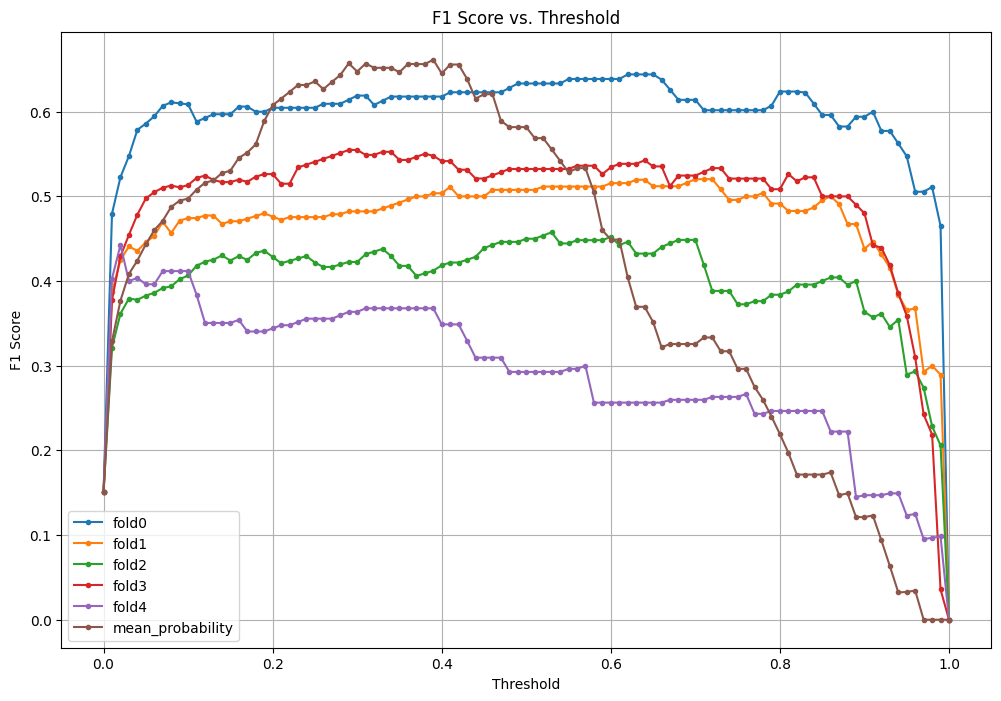
\includegraphics[width=1.0\linewidth]{Images/Chapter3/f1-vs-th-cls}
\caption{نمودار امتیاز \lr{F1} نسبت به آستانه برای \lr{Fold}ها و میانگین آنها}
\label{fig:ch3-f1-vs-th-cls}

\end{figure}


\begin{figure}[h!]
		\centering % <-- added
		\begin{subfigure}{0.45\textwidth}
			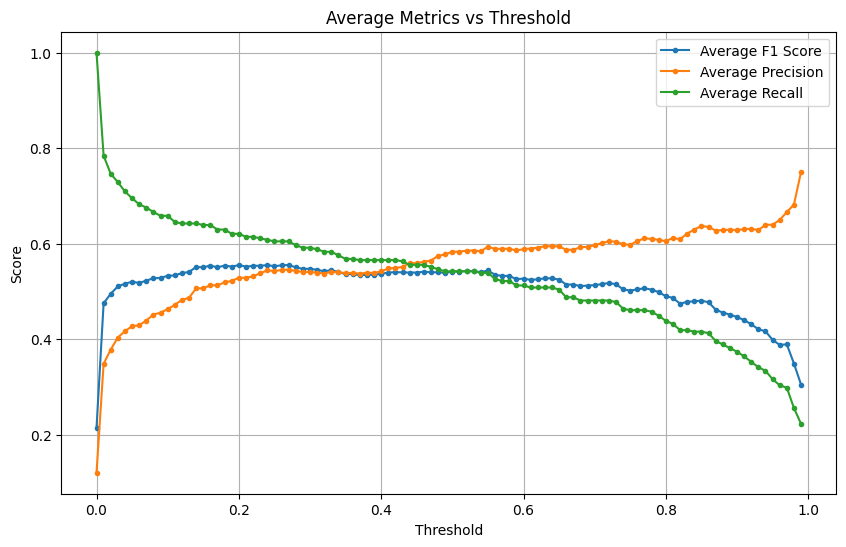
\includegraphics[width=\linewidth]{Images/Chapter3/metrics-cls.png}
			\caption{}
			
			\label{fig:ch3-metrics-cls}
		\end{subfigure}\hfil % <-- 
		\begin{subfigure}{0.45\textwidth}
			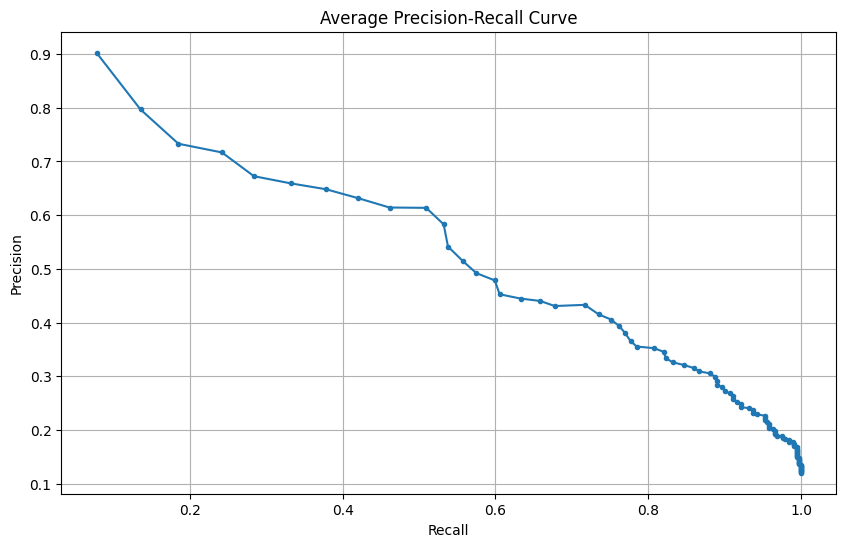
\includegraphics[width=\linewidth]{Images/Chapter3/pr-cls.png}
			\caption{}
			\label{fig:ch3-pr-cls}
		\end{subfigure}\hfil % <-- added
		\caption{نمودارهای سازوکار شورایی روی مجموعه‌داده ارزیابی}
		\label{fig:ch3-metrics and pr cls}
\end{figure}


\begin{figure}[h]
\centering
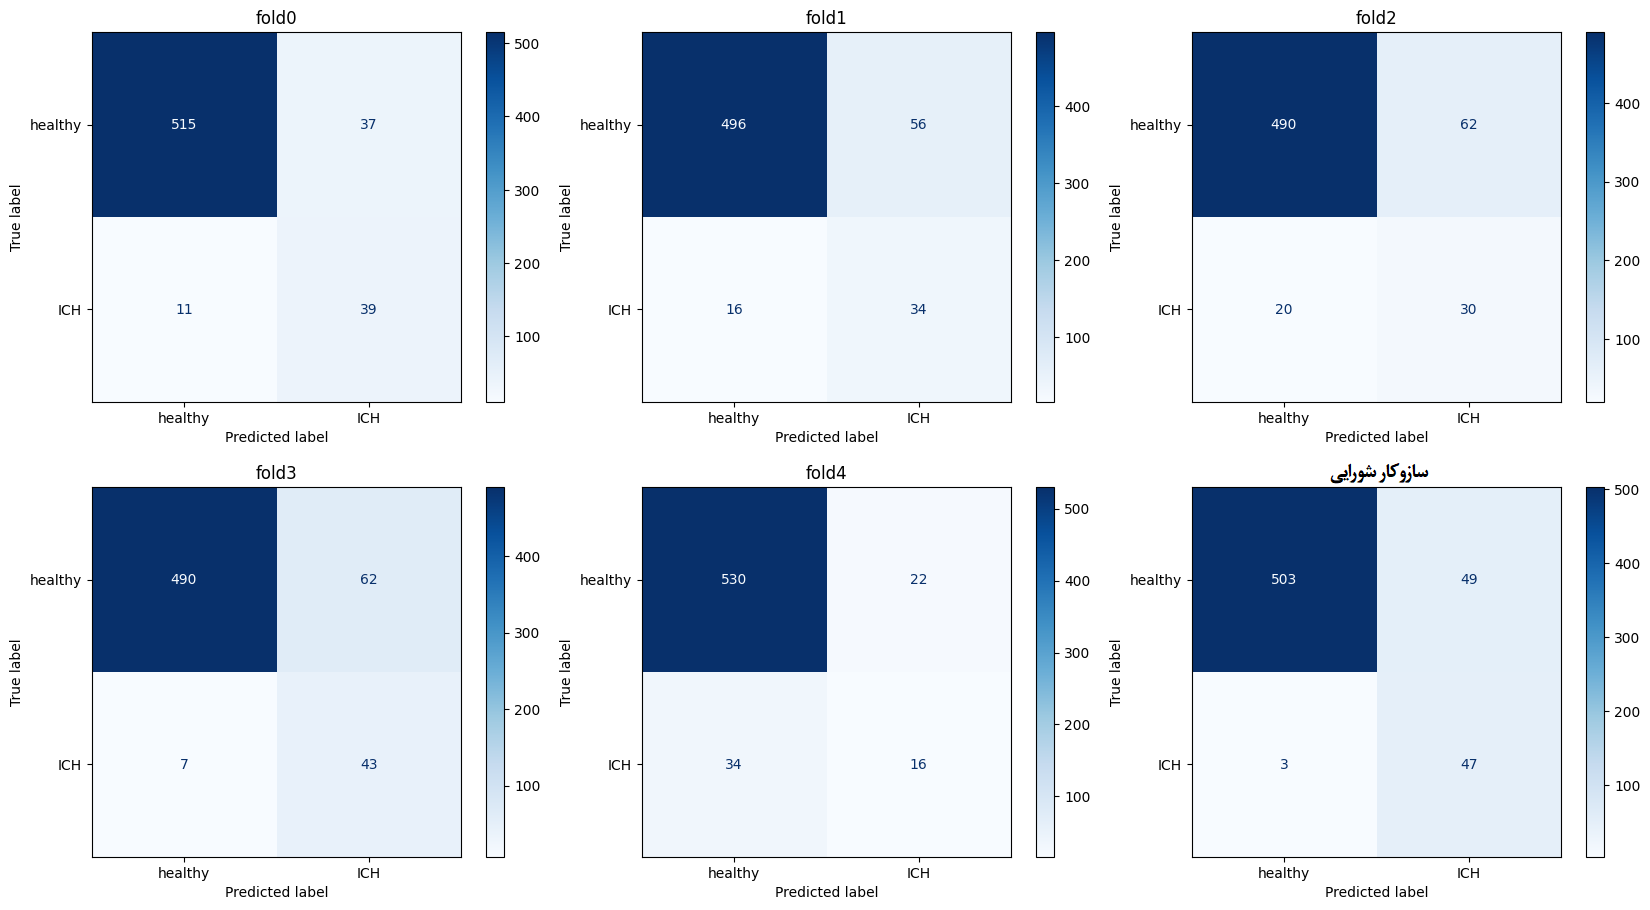
\includegraphics[width=1.0\linewidth]{Images/Chapter3/s-cm}
\caption{ماتریس آشفتگی نتایج برش‌محور}
\label{fig:ch3-s-cm}
\end{figure}


% Please add the following required packages to your document preamble:
% \usepackage{graphicx}
\begin{table}[]
\centering
\caption{نتیجه استفاده از فراپارامترهای بدست آمده از جستجوی شبکه‌ای روی مدل‌های دیگر}
\label{table:ch3-other models cls}
\resizebox{\textwidth}{!}{%
\begin{tabular}{lclllll}
\hline
\multicolumn{1}{c}{\textbf{مدل}} & \textbf{فراپارامتر پیشنهادی} & \textbf{\lr{Sensitivity}} & \textbf{\lr{Specificity}} & \textbf{\lr{Precision}} & \textbf{\lr{F1}} & \textbf{\lr{Accuracy}} \\ \hline
\lr{ResNet 50}      &  $\checkmark$                & $0.94$                 & $0.91$                 & $0.49$          & $0.64$          & $0.91$     \\
\lr{ResNet 50}      &      $\times$           & $0.76$                 & $0.78$                 & $0.23$          & $0.36$          & $0.77$     \\
\lr{VGG-16}         &   $\checkmark$               & $0.92$                 & $0.88$                 & $0.41$          & $0.56$          & $0.88$     \\
\lr{VGG-16}         &       $\times$          & $0.88$                 & $0.76$                 & $0.25$          & $0.39$          & $0.77$     \\
\lr{MobileNet-V2}   &   $\checkmark$               & $0.98$                 & $0.82$                 & $0.33$          & $0.50$          & $0.84$     \\
\lr{MobileNet-V2}   &      $\times$           & $\mathbf{1.00}$           & $\mathbf{0.68}$        & $\mathbf{0.22}$ & $\mathbf{0.36}$ & $0.71$     \\
\lr{Inception-V3}   &   $\checkmark$               & $0.64$                 & $0.90$                 & $0.36$          & $0.46$          & $0.88$     \\
\lr{Inception-V3}   &     $\times$            & $0.88$                 & $0.78$                 & $0.27$          & $0.41$          & $0.79$    
\\ \hline
\end{tabular}%
}
\end{table}


\subsection{نتایج بیمارمحور}

طبقه‌بندی بیمارمحور خونریزی درون‌جمجمه‌ای بر اساس پیش‌بینی‌های برش‌محور انجام شده است. یک بیمار در صورتی دارای خونریزی درون‌جمجمه‌ای در نظر گرفته می‌شود اگر حداقل یک برش از سی‌تی‌اسکن او دارای علائم خونریزی شناسایی شود. نتایج به‌دست‌آمده نشان می‌دهند که مدل 
\lr{ResNet50}
 در بررسی بیمارمحور سی‌تی‌اسکن‌ها، با استفاده از روش شورایی، به 
 \lr{Sensitivity}
  برابر با
   $1.00$، 
   \lr{Specificity}
برابر با
     $0.80$، \lr{Precision}
      برابر با
       $0.75$،
        امتیاز
         \lr{F1}
          برابر با
           $0.86$
            و 
            \lr{Accuracy}
             برابر با
              $0.88$ 
              دست‌یافته است که از تمامی معیارهای گزارش شده در سایر مطالعات، نتیجه بهتری کسب کرده است.
جدول \ref{tab:patient_level_results} نتایج بیمارمحور مدل \lr{ResNet50} را برای هر مرحله آموزشی نشان می‌دهد.
\autoref{fig:ch3-p-cm}
ماتریس آشفتگی بیمارمحور را نشان می‌دهد که از 16 بیمار در مجموعه ارزیابی قرار داشته‌اند که همه 6 بیمار دارای خونریزی درست تشخیص داده شده‌اند.

% Please add the following required packages to your document preamble:
% \usepackage{graphicx}
\begin{table}[]
\centering
\caption{نتایج بیمارمحور مدل \lr{ResNet50}
برای آستانه تصمیم‌گیری 
$0.27$}
\label{tab:patient_level_results}
\resizebox{\textwidth}{!}{%
\begin{tabular}{llllll}
\hline
\multicolumn{1}{c}{\textbf{مدل}}          & \textbf{\lr{Sensitivity}} & \textbf{\lr{Specificity}} & \textbf{\lr{Precision}} & \textbf{\lr{F1}}            & \textbf{\lr{Accuracy}}      \\ \hline
\lr{ResNet50 Fold 1}       & $1.00$                 & $0.60$                 & $0.60$               & $0.75$          & $0.75$          \\
\lr{ResNet50 Fold 2}       & $1.00$                 & $0.60$                 & $0.60$               & $0.75$          & $0.75$          \\
\lr{ResNet50 Fold 3}       & $1.00$                 & $0.60$                 & $0.60$               & $0.75$          & $0.75$          \\
\lr{ResNet50 Fold 4}       & $0.83$                 & $0.80$                 & $0.71$               & $0.77$          & $0.81$          \\ \hline
\lr{Kyung et al.}\cite{kyung2022improved} & $0.97$                 & $0.74$                 & $-$                  & $0.84$          & $-$             \\ \hline
\lr{ResNet50 Voting}       & $\mathbf{1.00}$        & $\mathbf{0.80}$        & $\mathbf{0.75}$      & $\mathbf{0.86}$ & $\mathbf{0.88}$
\\ \hline
\end{tabular}%
}
\end{table}
\begin{figure}[h]
\centering
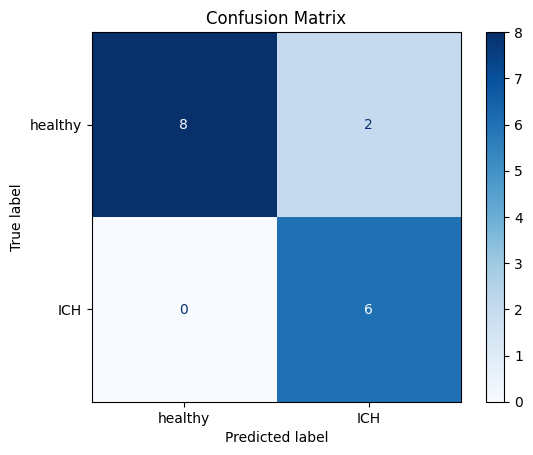
\includegraphics[width=1.0\linewidth]{Images/Chapter3/p-cm}
\caption{ماتریس آشفتگیب یمارمحور سازوکار شورایی}
\label{fig:ch3-p-cm}
\end{figure}


\subsection{تحلیل بیشتر نتایج}

در این بخش، نتایج مرتبط با تفسیرپذیری مدل \lr{ResNet50} از طریق روش‌های \lr{Grad-CAM} و \lr{t-SNE} تحلیل و بررسی می‌شوند.

\subsubsection{تحلیل \lr{Grad-CAM}}

روش 
\lr{Gradient-weighted Class Activation Mapping}
(\lr{Grad-CAM})
 به‌عنوان یک ابزار قدرتمند برای تفسیر مدل‌های شبکه عصبی عمیق استفاده می‌شود. این روش به ما اجازه می‌دهد تا ببینیم کدام بخش‌های تصویر ورودی، بیشتر در تصمیم‌گیری مدل تأثیر داشته‌اند. در این پروژه، از روش
 \lr{Grad-CAM}
  برای افزایش تفسیرپذیری مدل‌های طبقه‌بندی به کمک ایجاد تصویر استفاده شده است که نواحی مهم برش‌های سی‌تی‌اسکن که منجر به تشخیص خونریزی توسط مدل شده‌اند را مشخص می‌‌کند.  
  \autoref{fig:ch3-gradcam} 
  نمونه‌ای از این نقشه‌های حرارتی را نشان می‌دهد که به‌وضوح مشخص می‌کند که مدل چگونه نواحی مختلف تصویر را برای تشخیص \lr{ICH} مورد ارزیابی قرار داده است.
\begin{figure}[h]
\centering
\includegraphics[width=1.0\linewidth]{Images/Chapter3/GradCam}
\caption{چند نمونه از تصاویر تولید شده توسط  \lr{Grad-CAM}}
\label{fig:ch3-gradcam}
\end{figure}

\subsubsection{تحلیل \lr{t-SNE}}

روش
 \lr{t-Distributed Stochastic Neighbor Embedding} (\lr{t-SNE})
  یک روش برای کاهش ابعاد و تجسم داده‌های با ابعاد بالا است. در این پژوهش، از
   \lr{t-SNE}
    برای تجسم توزیع ویژگی‌های استخراج‌شده از مدل \lr{ResNet50} 
    استفاده شده است تا نشان داده شود که آموزش مدل، باعث تولید ویژگی‌هایی شده است که تفکیک‌پذیری برش‌های سالم را از ناسالم زیاد کرده است. 
     \autoref{fig:ch3-tsne}
 نشان‌دهنده توزیع ویژگی‌های استخراجی با روش 
 \lr{t-SNE}
  از تصاویر سی‌تی‌اسکن در فضای دو‌بعدی است که 
  \autoref{fig:ch3-tsne-before}
  پراکندگی ویژگی‌ها از مدل طبقه‌بندی قبل از آموزش آن است و 
    \autoref{fig:ch3-tsne-after}
    بعد از آموزش مدل طبقه‌بندی است. 
      \autoref{fig:ch3-tsne-before}
  به‌وضوح نشان می‌دهد چگونه مدل قادر است تفکیک‌پذیری خطی را برای برش‌های حاوی خونریزی درون‌جمجمه‌ای ایجاد کند. این استخراج ویژگی کمک می‌کند تا دیدگاه بهتری نسبت به نحوه عملکرد مدل در سطح ویژگی‌ها داشته باشیم و نقاط ضعف و قوت آن را بهتر درک کنیم. 
        \autoref{fig:ch3-tsne-other}
نمودار 
\lr{t-SNE}
حاصل از مدل طبقه‌بندی 
\lr{Ganeshkumar}\cite{Ganeshkumar2022Identification}
و همکاران است که نشان می‌دهد مدل به‌دست‌آمده در پژوهش آنها، امکان تفکیک‌پذیری خطی را برای برش‌ها ایجاد نکرده است.

\begin{figure}[h!]
		\centering % <-- added
		\begin{subfigure}{0.33\textwidth}
			\includegraphics[width=\linewidth]{Images/Chapter3/tsne_vanilla.png}
			\caption{قبل از آموزش}
			\label{fig:ch3-tsne-before}
		\end{subfigure}\hfil % <-- 
		\begin{subfigure}{0.33\textwidth}
			\includegraphics[width=\linewidth]{Images/Chapter3/tsne.png}
			\caption{بعد از آموزش}
			\label{fig:ch3-tsne-after}
		\end{subfigure}\hfil % <-- added
        \begin{subfigure}{0.33\textwidth}
			\includegraphics[width=\linewidth]{Images/Chapter3/tsne-other.png}
			\caption{مدل  
			\lr{Ganeshkumar} 
			\cite{Ganeshkumar2022Identification}}
			\label{fig:ch3-tsne-other}
        \end{subfigure}
		\caption{نمودارهای 
		\lr{t-SNE}
		و مقایسه آنها با یکدیگر}
		\label{fig:ch3-tsne}
\end{figure}


\section{نتایج قطعه‌بندی}
در این قسمت به بررسی نتایج حاصل شده از آموزش مدل قطعه‌بندی 
\lr{U-Net}و \lr{PSPNet}
 می‌پردازیم. نتیجه استفاده از جستجوی شبکه‌ای به روی مدل 
 \lr{‎U-Net}
 نشان می‌دهد که مدل با رمزگذار 
 \lr{SE-ResNeXt-101}
که با استفاده از تابع خطا
\lr{ِDice}
آموزش‌دیده و میزان برش‌های دارای خونریزی آن، 5 برابر شده است، بهترین نتیجه را به‌دست‌آورده‌. باتوجه به فراپارامتر‌هایی که در جستجوی شبکه‌ای مدل
 \lr{‎U-Net}
 به‌دست‌آمد، مدل
 \lr{PSPNet}
 آموزش داده شد تا نشان دهیم این فراپارامترها می‌توانند عملکرد مدل‌های قطعه‌بندی را بهبود بخشند. 
 \autoref{fig:ch3-seg-training-graph}
 منحنی‌های مربوط به آموزش مدل روی 
 \lr{Fold 1}
را نشان می‌دهد که در آن 
 \texttt{Original test without post-process}،
 مربوط به مجموعه‌داده ارزیابی است که از مدل طبقه‌بندی عبور داده نشده است و عملیات پس‌پردازش به روی آن انجام نشده است.
 منحنی 
 \texttt{Original test with post-process}
 مربوط به مجموعه‌داده ارزیابی است که از مدل طبقه‌بندی عبور داده نشده‌ است؛ اما عملیات پس‌پردازش به روی آن انجام شده است.
منحنی 
 \texttt{Reduced test with post-process}
 مربوط به مجموعه‌داده ارزیابی است که از مدل طبقه‌بندی عبور داده شده و عملیات پس‌پردازش به روی آن انجام شده است.
 همان‌طور که از نمودارهای مربوط به معیار
 \lr{IoU}
 در 
 \autoref{fig:ch3-seg-IoU}
 و معیار 
 \lr{Dice}
  در 
  \autoref{fig:ch3-seg-Dice}
  مشخص است،‌ پس‌پردازش پیشنهادی و روش دومرحله‌ای هرکدام باعث بهبود چشمگیر نتایج مدل شبکه عصبی شده‌اند.
 
 \begin{figure}[h!]
 		\centering % <-- added
 		\begin{subfigure}{0.49\textwidth}
 			\includegraphics[width=\linewidth]{Images/Chapter3/seg-IoU-metrics.png}
 			\caption{\lr{IoU}}
 			\label{fig:ch3-seg-IoU}
 		\end{subfigure}\hfil % <-- 
 		\begin{subfigure}{0.49\textwidth}
 			\includegraphics[width=\linewidth]{Images/Chapter3/seg-Dice-metrics.png.png}
 			\caption{\lr{Dice}}
 			\label{fig:ch3-seg-Dice}
 		\end{subfigure}\hfil % <-- added
 		\caption{یک نمونه از عملکرد روش پیشنهادی و پس‌پردازش در فرایند آموزش }
 		\label{fig:ch3-seg-training-graph}
 \end{figure}
 
 با درنظرگرفتن کمترین مقدار تابع خطا، بهترین
 \lr{Epoch}
 هر 
 \lr{Fold}
 انتخاب می‌شود و پس از آن برای تنظیم متغیرهای مربوط به سازوکار شورا، نمودارهای 
 \lr{ِIoU}
 و 
 \lr{Dice}
 نسبت به آستانه‌های متفاوت رسم می‌شود و بهترین آستانه به دست می‌آید.
 
 \autoref{table:ch3-seg-results}
 نتایج 
 \lr{ّFold}ها،
 روش شورایی و تحقیقات گذشته را نشان می‌دهد. همان‌طور که مشخص است روش مذکور توانسته معیار
 \lr{Dice}
 را نسبت به مطالعات پیشین بهبود ببخشید درحالی‌که مقدار 
 \lr{IoU}
 آن نیز به‌صورت کلی از آنها بهتر است.

 \begin{table}[]
 \centering
 \caption{نتایج قطعه‌بندی تصاویر سی‌تی‌اسکن}
 \label{table:ch3-seg-results}
  \adjustbox{width=0.8\columnwidth,max totalheight=\textheight, keepaspectratio}{
 \begin{tabular}{rllll}
 \hline
 \textbf{مدل} & \textbf{} & \multicolumn{1}{r}{\textbf{\lr{IoU}}}  & \textbf{} & \multicolumn{1}{r}{\textbf{\lr{Dice}}} \\ \cline{2-5}
                                                  & عادی      & دو مرحله‌ای    & عادی      & دو مرحله‌ای    \\ \hline
 \lr{U-Net Fold 0}                                                       & $0.12$      & $0.21$          & $0.21$      & $0.35$          \\
 \lr{PSPNet Fold 0}                                                       & $0.18$      & $0.22$          & $0.31$      & $0.36$          \\
 \lr{U-Net Fold 1}                                                       & $0.17$      & $0.20$          & $0.29$      & $0.34$          \\
 \lr{PSPNet Fold 1}                                                       & $0.17$      & $0.21$          & $0.29$      & $0.35$          \\
 \lr{U-Net Fold 2}                                                       & $0.06$      & $0.20$          & $0.12$      & $0.33$          \\
 \lr{PSPNet Fold 2}                                                       & $0.11$      & $0.16$          & $0.20$      & $0.28$          \\
 \lr{U-Net Fold 3}                                                       & $0.19$      & $0.19$          & $0.16$      & $0.32$          \\
 \lr{PSPNet Fold 3}                                                       & $0.20$      & $0.23$          & $0.34$      & $0.37$          \\
 \lr{U-Net Fold 4}                                                       & $0.09$      & $0.19$          & $0.16$      & $0.33$          \\ 
 \lr{PSPNet Fold 4}                                                       & $0.16$      & $0.21$          & $0.27$      & $0.35$          \\
  \hline
 \lr{U-Net Hssayeni}\cite{hssayeni2020intracranial}                                                          & $0.22$      & -             & $0.32$      & -             \\
 \lr{U-Net Neethi}\cite{neethi2022stroke}                                                          & $0.20$      & -             & $0.35$      & -             \\ \hline
 \lr{U-Net} شورایی
                                                        & $0.17$      & $0.22$ & $0.29$      & $0.36$\\
\lr{PSPNet} شورایی
                                                        & $0.20$      & \textbf{$0.23$} & $0.34$      & \textbf{$0.38$}
 \\ \hline
 \end{tabular}%
 }
 \end{table}
 
 
 
 
 
 \autoref{fig:dice-th-seg-unet} و \autoref{fig:dice-th-seg-psp}
 نتایج 
  \lr{ِIoU}
  و 
  \lr{Dice}
 را به‌ازای آستانه‌های متفاوت برای دو مدل
 \lr{U-Net} و \lr{PSPNet}
 نشان می‌دهند. همان‌طور که مشخص است، میانگین عملکرد مدل‌ها به روی زیرمجموعه اعتبارسنجی که توزیع برش‌های آن، مشابه با توزیع برش‌ها در زیرمجموعه ارزیابی است، بسیار بیشتر از نتایج به‌دست‌آمده به روی زیرمجموعه ارزیابی است. علت اصلی این تفاوت، در توزیع مکانی خونریزی درون‌جمجمه‌ای موجود در زیرمجموعه ارزیابی نسبت به بقیه زیر‌مجموعه‌ها است که در 
 \autoref{fig:heatmaps}
 این تفاوت توزیع مشخص است. 
 \lr{Hssayeni}\cite{hssayeni2020intracranial} 
 و همکاران، در پژوهشی که نتایج آن در
 \autoref{table:ch3-seg-results}
 آورده شده است، نتایج خود را از میانگین گرفتن از نتایج به‌دست‌آمده از هر
 \lr{Fold}
 گزارش کرده‌اند؛ بنابراین اگر این معیار را برای ارزیابی نتایج روش دومرحله‌ای در نظر بگیریم، این روش بهبود قابل‌توجهی در معیارهای قطعه‌بندی ایجاد کرده است.
 
 
\begin{figure}[h]
\centering
\includegraphics[width=1.0\linewidth]{Images/Chapter3/dice-th-seg}
\caption{نتایج مدل
\lr{U-Net}
به‌ازای آستانه‌های متفاوت}
\label{fig:dice-th-seg-unet}
\end{figure}
 
 
  \begin{figure}[h!]
  		\centering % <-- added
  		\begin{subfigure}{0.49\textwidth}
  			\includegraphics[width=\linewidth]{Images/Chapter3/IoU-th-seg-psp.jpg}
  			\caption{\lr{IoU}}
  			\label{fig:ch3-seg-IoU-psp}
  		\end{subfigure}\hfil % <-- 
  		\begin{subfigure}{0.49\textwidth}
  			\includegraphics[width=\linewidth]{Images/Chapter3/Dice-th-seg-psp.jpg}
  			\caption{\lr{Dice}}
  			\label{fig:ch3-seg-Dice-psp}
  		\end{subfigure}\hfil % <-- added
\caption{نتایج مدل
\lr{PSPNet}
به‌ازای آستانه‌های متفاوت}
  		\label{fig:dice-th-seg-psp}
  \end{figure}
  
\chapter{توضیحات و نتیجه‌گیری}
\section{توضیحات}
خونریزی درون‌جمجمه‌ای یک وضعیت اضطراری پزشکی است که به دلایل متفاوت مثل آسیب‌های مغزی تروماتیک، بیماری‌های عروقی یا مشکلات مادرزادی ایجاد شود\cite{monica2022detection}.
جلوگیری از مرگ و کاهش عوارض ایجاد شده در خونریزی درون‌جمجمه‌ای نیازمند مداخله سریع است؛ اما به علت وجود عوامل محیطی مانند شلوغی مراکز درمان یا نبود متخصص مربوطه، تشخیص و درمان بیمار دارای خونریزی درون‌جمجمه‌ای می‌تواند با تأخیر انجام شود. علاوه‌بر این بررسی تصاویر پیچیده و سه‌بعدی سی‌تی‌اسکن نیز یکی دیگر از چالش‌ها در تشخیص دستی خونریزی درون‌جمجمه‌ای است.

این پژوهش در گام نخست با استفاده یک روش پردازش تصاویر سی‌تی‌اسکن مبتنی بر شبکه‌های عصبی عمیق،‌ یک دستیار هوشمند را برای استفاده در مراکز پزشکی توسعه داده و در گام بعدی با توسعه روش‌های موجود در پردازش تصاویر سی‌تی‌اسکن، دقت این دستیار را در زمینه طبقه‌بندی و قطعه‌بندی افزایش داده است.
استفاده از روش دومرحله‌ای موجب کاهش
\lr{Field-of-View}
در مدل قطعه‌بندی به 
\lr{Region-of-Interest}
می‌شود که در نتیجه آن، امکان ایجاد خطا در برش‌‌های سالم کاهش پیدا می‌کند. از دیگر روش‌های دومرحله‌ای به 
\lr{Cascaded U-Net}
و روش
\lr{Fine to coarse}
می‌توان اشاره کرد.
 نتایج به‌دست‌آمده از روش دومرحله‌ای پیشنهاد شده در این پژوهش به همراه پس‌پردازش استفاده شده،‌ نشان داد که عملکرد مدل می‌تواند بهبود قابل‌توجهی پیدا بکند که نشان‌دهنده این است که این روش می‌تواند در مراکز پزشکی استفاده شود.

بااین‌حال، چالش‌ها و محدودیت‌هایی در این تحقیق وجود دارد. یکی از مهم‌ترین چالش‌ها، دسترسی محدود به مجموعه‌داده‌های متنوع و بزرگ در حوزه طبقه‌بندی و قطعه‌بندی خونریزی درون‌جمجمه‌ای است. تنوع ناکافی در کیفیت تصاویر سی‌تی‌اسکن نیز ممکن است بر قابلیت تعمیم‌پذیری مدل‌های ما تأثیر بگذارد. همچنین، توان محاسباتی موردنیاز برای آموزش مدل‌ها و اجرای پس‌پردازش ممکن است باعث افزایش زمان پردازش شود که باید در آینده با استفاده از روش‌های بهینه‌سازی بهبود یابد.
یکی از محدودیت‌های اساسی در این پژوهش این است که برای پردازش یک تصویر سی‌تی‌اسکن،‌ لازم است تا این تصویر از 10 مدل شبکه عصبی عبور داده شود و سازوکار شورایی روی آنها اعمال شود که این مسئله توان محاسباتی موردنیاز را افزایش می‌دهد.

یکی از مهم‌ترین زمینه‌های موجود برای پژوهش‌های آینده، جمع‌آوری یکم مجموعه‌داده باکیفیت و حجم مناسب از مراکز موجود در ایران است که با استفاده از این مجموعه‌داده امکان ارزیابی عملکرد مدل در مراکز بهداشتی ایران فراهم شود. در ادامه استفاده از مجموعه‌داده‌های موجود مثل
\lr{RSNA}\cite{rsna_hemorrhage_detection_kaggle}
که تعداد بسیار زیادی تصویر مناسب برای طبقه‌بندی دارد و استفاده از روش‌های انتقال آموزش،‌ می‌تواند یکی از راه‌های بهبود عملکرد مدل‌های پردازش تصویر باشد. 
ازآنجایی‌که تصاویر سی‌تی‌اسکن یک توالی از برش‌ها است، اضافه‌کردن لایه‌های زمانی در مراحل تصمیم‌گیری می‌تواند در عملکرد مدل تأثیرگذار باشد. تصاویر سی‌تی‌اسکن ماهیت سه‌بعدی دارند؛ بنابراین توسعه مدل‌هایی که از لایه‌های پیچشی سه‌بعدی استفاده کنند یا روش‌های 
$2D+1D$
به‌منظور افزایش مشارکت برش‌ها در تصمیم‌گیری مدل یک زمینه تحقیقاتی است.
استفاده از مدل‌های جدید در زمینه پردازش تصاویر خصوصاً مدل‌های مبتنی بر مکانیزم 
\LTRfootnote{Mechanism}
توجه و مدل‌هایی که حساسیت آنها به شکل ضایعه بیشتر از بافت ضایعه باشد یکی از زمینه‌های موجود برای پژوهش‌های آینده است.
روش 
\lr{Model soups}
نیز می‌تواند یک زمینه جذاب برای توسعه عملکرد مدل‌ها برای استفاده در زمینه پزشکی باشد. 
توسعه سازوکار شورایی،‌ یک زمینه مناسب برای توسعه عملکرد مدل‌ها است،‌به توجه به اینکه آستانه بهینه برای هر مدل می‌تواند با مدل دیگر متفاوت باشد،‌ استفاده از روش‌هایی مبتنی بر ریاضیات فازی 
\LTRfootnote{Fazzy}
یک پیشنهاد مناسب برای مواجهه با این چالش است. زمینه پیشنهادی دیگر برای پردازش تصاویر سی‌تی‌اسکن، تغییر ساختار روش دومرحله‌ای از یک مدل طبقه‌بندی به همراه یک مدل قطعه‌بندی، به یک مدل بخش‌بندی به همراه یک مدل قطعه‌بندی است. این روش با شناسایی محدوده خونریزی، ناترازی پیکسلی را به‌منظور آموزش مدل قطعه‌بندی کاهش می‌دهد. 
 
\section{نتیجه‌گیری}
در این پایان‌نامه، یک روش دومرحله‌ای برای شناسایی و قطعه‌بندی خودکار خونریزی‌های درون‌جمجمه‌ای با استفاده از تصاویر سی‌تی‌اسکن ارائه شده است. استفاده از روش پس‌پردازش و تصمیم‌گیری پس از قطعه‌بندی، بهبود قابل‌توجهی در دقت و صحت نتایج داشته است. نتایج به‌دست‌آمده نشان می‌دهد که این روش می‌تواند به‌عنوان یک ابزار کارآمد در تشخیص‌های پزشکی به کار رود.
باتوجه‌به نتایج حاصل از این پژوهش، ابزار‌های هوش مصنوعی و یادگیری عمیق می‌توانند نقشی اساسی در بهبود کیفیت تشخیص‌های پزشکی داشته باشند. در آینده، می‌توان این مدل را با استفاده از مجموعه‌داده‌های متنوع‌تر و روش‌های پیچیده‌تر مانند استفاده از مکانیسم‌های توجه گسترش داد. همچنین، امکان ادغام این مدل با فرایند‌های بیمارستانی برای تشخیص زمان‌واقعی و کمک به تصمیم‌گیری پزشکان وجود دارد.
این پژوهش نشان می‌دهد که ادغام مدل‌های هوش مصنوعی با فرایند‌های پزشکی می‌تواند به بهبود کارایی و کاهش زمان و هزینه‌های تشخیص و درمان کمک کند. با توسعه بیشتر این مدل‌ها، استفاده گسترده‌تر از آن‌ها در بیمارستان‌ها و مراکز درمانی ممکن است منجر به بهبود نتایج بیماران و کاهش خطاهای پزشکی شود.

%\include{chapter5}
%\include{chapter6}


%--------------------------------------------------------------------------appendix( مراجع و پیوست ها)

\chapterfont{\vspace*{-2em}\centering\LARGE}%

\appendix
\bibliographystyle{unsrt-fa}
\bibliography{references}
%\include{appendix1}
%--------------------------------------------------------------------------dictionary(واژه نامه ها)
%اگر مایل به داشتن صفحه واژه‌نامه نیستید، خط زیر را غیر فعال کنید.
\parindent=0pt
%
\chapter*{واژه‌نامه‌ی فارسی به انگلیسی}
\pagestyle{style9}

\addcontentsline{toc}{chapter}{واژه‌نامه‌ی فارسی به انگلیسی}
%%%%%%
\begin{multicols*}{2}
{\bf الف}
\farsiTOenglish{آسیب مغزی تروماتیک}{Traumatic brain injury}
\farsiTOenglish{اتصال میانبر }{Skip Connection}
\farsiTOenglish{ادغام }{Pooling}
\farsiTOenglish{ارزیابی }{Test}
\farsiTOenglish{اعتبار سنجی }{Validation}
\farsiTOenglish{الحاق }{concatenation}
\farsiTOenglish{الکترون }{Electron}
\farsiTOenglish{انتقال یادگیری}{Transfer Learning}
\farsiTOenglish{انقجار مشتق }{Exploding Gradient}
\farsiTOenglish{اشعه ایکس}{X-Ray}
\farsiTOenglish{افزایش مصنوعی داده}{Augmentation}


{\bf ب}
\farsiTOenglish{بایاس‌}{Bias}
\farsiTOenglish{برش}{Slice}
\farsiTOenglish{برش‌محور}{Slice-wise}
\farsiTOenglish{بلوک}{Block}
\farsiTOenglish{بیش‌برازش}{Overfit}
\farsiTOenglish{بیمار‌محور}{Patient-wise}


{\bf پ}
\farsiTOenglish{پرتونگاری}{Radiography}
\farsiTOenglish{پرتونگار }{Radiologist}
\farsiTOenglish{پرسپترون }{Perceptron}
\farsiTOenglish{پس‌انتشار}{backpropagation}
\farsiTOenglish{پس‌پردازش}{Post-process}
\farsiTOenglish{‌پنجره‌گذاری}{Windowing}
\farsiTOenglish{پیش‌پردازش}{Pre-process}
\farsiTOenglish{پیکسل}{pixel}

{\bf ت}
\farsiTOenglish{تابع خطا‌}{Loss Function}


{\bf ج}
%%\vspace*{3mm}
\farsiTOenglish{جاگذاری داده}{Bootstrap}
\farsiTOenglish{‌جستجوی شبکه‌ای}{Grid Search}

{\bf ح}
%%\vspace*{3mm}
\farsiTOenglish{حاشیه‌نویسی}{Annotation}


{\bf خ}
%%\vspace*{3mm}
\farsiTOenglish{خودرمزگذار}{Autoencoder}
\farsiTOenglish{خونریزی}{Hemorrhage}
\farsiTOenglish{خونریزی درون‌جمجمه‌ای}{Intracerebral Hemorrhage (ICH)}
\farsiTOenglish{خونریزی اپیدورال}{Epidural Hemorrhage}
\farsiTOenglish{خونریزی ساب‌دورال}{Subdural Hemorrhage}
\farsiTOenglish{ساب‌آراکنوئید}{Subarachnoid Hemorrhage}
\farsiTOenglish{خونریزی پارانشیم مغزی}{Cerebral Parenchymal Hemorrhage}
\farsiTOenglish{خونریزی داخل بطنی}{Intraventricular Hemorrhage}

{\bf ر}
%%\vspace*{3mm}
\farsiTOenglish{رایانه}{Computer}

{\bf ز}
%%\vspace*{3mm}
\farsiTOenglish{زمان واقعی }{Real Time}


{\bf س}
%%\vspace*{3mm}
\farsiTOenglish{سی‌تی‌اسکن }{Computed Tomography Scan}
\farsiTOenglish{سامانه }{System}

{\bf ش}
%%\vspace*{3mm}
\farsiTOenglish{شبکه عصبی عمیق }{Deep Neural Network}
\farsiTOenglish{شبکه عصبی پیچشی }{Convolutional Neural Network}
\farsiTOenglish{شورا }{Voting}
{\bf ط}
%%\vspace*{3mm}
\farsiTOenglish{طبقه‌بندی}{Classification}


{\bf غ}
%%\vspace*{3mm}
\farsiTOenglish{غیر تهاجمی}{Non-invasive}

{\bf ف}
%%\vspace*{3mm}
\farsiTOenglish{‌‌فراپارامتر}{Hyper-parameter}



{\bf ق}
%%\vspace*{3mm}
\farsiTOenglish{قطعه‌‌بندی}{Segmentation}


{\bf ک}
%%\vspace*{3mm}
\farsiTOenglish{کاتد}{Cathode  }
\farsiTOenglish{کانال}{Channel  }
\farsiTOenglish{کاردینالیتی}{Cardinality  }
\farsiTOenglish{کالیبراسیون}{Calibration}
\farsiTOenglish{کاهش داده غالب}{Undersampling}



{\bf گ}
%%\vspace*{3mm}
\farsiTOenglish{گرادیان}{Gradient}



{\bf م}
%%\vspace*{3mm}
\farsiTOenglish{ماسک}{Mask}
\farsiTOenglish{مدل}{Model}


{\bf ن}
%%\vspace*{3mm}
\farsiTOenglish{ناپدیدشدن مشتق }{Vanishing Gradient}
\farsiTOenglish{نرون }{Neuron}
\farsiTOenglish{نظر ثانویه}{Second Opinion}
\farsiTOenglish{نقشه ویژگی}{Feature Map}


{\bf ی}
%%\vspace*{3mm}
\farsiTOenglish{وضوح }{Resolution}


{\bf ی}
%%\vspace*{3mm}
\farsiTOenglish{یادگیری عمیق}{Deep Learning}
\farsiTOenglish{یادگیری ماشین}{Machine Learning}

\end{multicols*}


%
%%%%%%
\chapter*{ واژه‌نامه‌ی انگلیسی به فارسی}
\pagestyle{style9}
\lhead{\thepage}\rhead{واژه‌نامه‌ی انگلیسی به فارسی}
\addcontentsline{toc}{chapter}{واژه‌نامه‌ی انگلیسی به فارسی}

\LTRmulticolcolumns
\begin{multicols}{2}
{\bf \lr{A}}
\englishTOfarsi{Annotation}{حاشیه‌نویسی}
\englishTOfarsi{Augmentation}{افزایش مصنوعی داده}
\englishTOfarsi{Autoencoder}{خودرمزگذار}

{\bf \lr{B}}
\englishTOfarsi{Backpropagation}{پس‌انتشار}
\englishTOfarsi{Bias}{بایاس‌}
\englishTOfarsi{Block}{بلوک}
\englishTOfarsi{Bootstrap}{جاگذاری داده}

{\bf \lr{C}}
\englishTOfarsi{Calibration}{کالیبراسیون}
\englishTOfarsi{Cardinality}{کاردینالیتی}
\englishTOfarsi{Cathode}{کاتد}
\englishTOfarsi{Cerebral Parenchymal Hemorrhage}{خونریزی پارانشیم مغزی}
\englishTOfarsi{Channel}{کانال}
\englishTOfarsi{Classification}{طبقه‌بندی}
\englishTOfarsi{Computed Tomography Scan}{سی‌تی‌اسکن}
\englishTOfarsi{Concatenation}{الحاق}
\englishTOfarsi{Computer}{رایانه}
\englishTOfarsi{Convolutional Neural Network}{شبکه عصبی پیچشی}

{\bf \lr{D}}
\englishTOfarsi{Deep Learning}{یادگیری عمیق}
\englishTOfarsi{Deep Neural Network}{شبکه عصبی عمیق}

{\bf \lr{E}}
\englishTOfarsi{Electron}{الکترون}
\englishTOfarsi{Epidural Hemorrhage}{خونریزی اپیدورال}
\englishTOfarsi{Exploding Gradient}{انقجار مشتق}

{\bf \lr{F}}
\englishTOfarsi{Fuzzy}{فازی}
\englishTOfarsi{Feature Map}{نقشه ویژگی}

{\bf \lr{G}}
\englishTOfarsi{Gradient}{گرادیان}
\englishTOfarsi{Grid Search}{‌جستجوی شبکه‌ای}

{\bf \lr{H}}
\englishTOfarsi{Hemorrhage}{خونریزی}
\englishTOfarsi{Hyper-parameter}{‌فراپارامتر}

{\bf \lr{I}}
\englishTOfarsi{Intraventricular Hemorrhage}{خونریزی داخل بطنی}
\englishTOfarsi{Intracerebral Hemorrhage (ICH)}{خونریزی درون‌جمجمه‌ای}

{\bf \lr{L}}
\englishTOfarsi{Loss Function}{تابع خطا‌}

{\bf \lr{M}}
\englishTOfarsi{Machine Learning}{یادگیری ماشین}
\englishTOfarsi{Mask}{ماسک}
\englishTOfarsi{Mechanism}{مکانیزم}
\englishTOfarsi{Model}{مدل}

{\bf \lr{N}}
\englishTOfarsi{Neuron}{نرون}
\englishTOfarsi{Non-invasive}{غیر تهاجمی}

{\bf \lr{O}}
\englishTOfarsi{Overfit}{بیش‌برازش}

{\bf \lr{P}}
\englishTOfarsi{Patient-wise}{بیمار‌محور}
\englishTOfarsi{Perceptron}{پرسپترون}
\englishTOfarsi{Pixel}{پیکسل}
\englishTOfarsi{Pooling}{ادغام}
\englishTOfarsi{Post-process}{پس‌پردازش}
\englishTOfarsi{Pre-process}{پیش‌پردازش}

{\bf \lr{R}}
\englishTOfarsi{Radiography}{پرتونگاری}
\englishTOfarsi{Radiologist}{پرتونگار}
\englishTOfarsi{Real Time}{زمان واقعی}
\englishTOfarsi{Resolution}{وضوح}

{\bf \lr{S}}
\englishTOfarsi{Segmentation}{قطعه‌‌بندی}
\englishTOfarsi{Second Opinion}{نظر ثانویه}
\englishTOfarsi{Skip Connection}{اتصال میانبر}
\englishTOfarsi{Slice}{برش}
\englishTOfarsi{Slice-wise}{برش‌محور}
\englishTOfarsi{Subarachnoid Hemorrhage}{ساب‌آراکنوئید}
\englishTOfarsi{Subdural Hemorrhage}{خونریزی ساب‌دورال}
\englishTOfarsi{System}{سامانه}

{\bf \lr{T}}
\englishTOfarsi{Test}{ارزیابی}
\englishTOfarsi{Traumatic brain injury}{آسیب مغزی تروماتیک}
\englishTOfarsi{Transfer Learning}{انتقال یادگیری}

{\bf \lr{U}}
\englishTOfarsi{Undersampling}{کاهش داده غالب}

{\bf \lr{V}}
\englishTOfarsi{Validation}{اعتبار سنجی}
\englishTOfarsi{Vanishing Gradient}{ناپدیدشدن مشتق}
\englishTOfarsi{Voting}{شورا}

{\bf \lr{W}}
\englishTOfarsi{Windowing}{‌پنجره‌گذاری}

{\bf \lr{X}}
\englishTOfarsi{X-Ray}{اشعه ایکس}

\end{multicols}
%--------------------------------------------------------------------------index(نمایه)
%اگر مایل به داشتن صفحه نمایه نیستید، خط زیر را غیر فعال کنید.
\pagestyle{style7}
\printindex
\pagestyle{style7}
%کلمات کلیدی انگلیسی
\latinkeywords{Deep Neural Network, CT Scan Image Classification, CT Scan Image Segmentation, Intracranial Hemorrhage}
%چکیده انگلیسی

\en-abstract{
The rapid and accurate detection of intracranial hemorrhages using CT scan images has consistently been recognized as one of the most significant medical challenges in treating individuals with various brain injuries, strokes, and intracranial hemorrhages. The importance of this issue becomes apparent when even a few minutes of delay in diagnosis can lead to irreversible consequences for patients.
Given the complexity and high sensitivity of diagnosing such injuries, this process typically requires a high level of expertise and experience from physicians and radiologists. However, due to the limitations of human resources and the potential for human error, the need for the development of automated diagnostic systems based on deep learning has become increasingly evident.
In this context, the primary challenge for physicians, especially in emergency departments, is the accurate and rapid detection of hemorrhage regions in three-dimensional CT scan images. The performance of specialists in analyzing these images is influenced by their level of experience and environmental conditions.
The development of an intelligent assistant based on deep neural networks can improve medical processes in this area; however, developing such an assistant faces several challenges. Among these challenges are data imbalance, limited access to large datasets, and the variation in CT scan image quality across different imaging centers. These factors can reduce the accuracy of models in detecting hemorrhagic regions.
In this research, a two-stage method based on classification and segmentation, along with a post-processing step, has been developed using the PhysioNet intracranial hemorrhage dataset. In this research, the ResNet-50 model was used in the first stage and the U-Net model in the second stage, resulting in an IoU score of 0.22 and a Dice coefficient of 0.36. These results represent a significant improvement compared to the case where the two-stage method was not utilized.
}
%%%%%%%%%%%%%%%%%%%%% کدهای زیر را تغییر ندهید.

\newpage
\thispagestyle{empty}
\begin{latin}
\section*{\LARGE\centering Abstract}

\een-abstract

\vspace*{.5cm}
{\large\textbf{Key Words:}}\par
\vspace*{.5cm}
\elatinkeywords
\end{latin}
% در این فایل، عنوان پایان‌نامه، مشخصات خود و چکیده پایان‌نامه را به انگلیسی، وارد کنید.
%%%%%%%%%%%%%%%%%%%%%%%%%%%%%%%%%%%%
\baselineskip=.6cm
\begin{latin}

\latinfaculty{Department of Electrical Engineering}


\latintitle{Processing Brain CT‌ Scan Images for Interacerbal Brain Hemorrhage with Deep Neural Network}


\firstlatinsupervisor{Dr. Amirhossein Nikoofard}

%\secondlatinsupervisor{Second Supervisor}

%\firstlatinadvisor{Dr. }

%\secondlatinadvisor{Second Advisor}

\latinname{Seyed Mohammad}

\latinsurname{Hoseyni}

\latinthesisdate{September \& 2024}

\latinvtitle
\end{latin}

\end{document}